%%%%%%%%%%%%%%%%%%%%%%%%%%%%% Thesis.tex %%%%%%%%%%%%%%%%%%%%%%%%%%%%%%%
%                                                                      %
%  ---------- Master of Science Dissertation template ----------       %
%                                                                      %
%  Template for the Master Thesis according to the regulations         %
%  published by the Academic Board (Direcção Académica) at IST.        %
%                                                                      %
%  For up-to-date guide, please refer to the offical website           %
%  http://da.tecnico.ulisboa.pt/dissertacao-de-mestrado/               %
%                                                                      %
%       Andre C. Marta                                                 %
%       Area Cientifica de Mecanica Aplicada e Aeroespacial            %
%       Departamento de Engenharia Mecanica                            %
%       Instituto Superior Tecnico                                     %
%       Av. Rovisco Pais                                               %
%       1049-001 Lisboa                                                %
%       Portugal                                                       %
%       Tel: +351 21 841 9469                                          %
%                        3469 (extension)                              %
%       Email: andre.marta@tecnico.ulisboa.pt                          %
%                                                                      %
%  Created:       Jan 20, 2011                                         %
%  Last Modified: May  7, 2014                                         %
%                                                                      %
%%%%%%%%%%%%%%%%%%%%%%%%%%%%%%%%%%%%%%%%%%%%%%%%%%%%%%%%%%%%%%%%%%%%%%%%
%  Revision history                                                    %
%  v1 - 2011/01/24 - original template                                 %
%  v2 - 2012/10/30 - new IST image and glossary support                %
%  v3 - 2013/12/10 - update according to 2012/13 official guide        %
%  v4 - 2014/02/28 - new default for bibliography style                %
%  v5 - 2014/05/07 - update according to 2013/14 official guide        %
%%%%%%%%%%%%%%%%%%%%%%%%%%%%%%%%%%%%%%%%%%%%%%%%%%%%%%%%%%%%%%%%%%%%%%%%
%                                                                      %
% To generate the PDF file, type "make" at the terminal prompt.        %
%                                                                      %
% The IST template LaTeX package was created by the author             %
% and it can be downloaded from:                                       %
% https://fenix.ist.utl.pt/homepage/ist31052/                          %
%                                                                      %
% The external packages can be downloaded from                         %
% the Comprehensive TeX Archive Network at http://www.ctan.org/        %
%                                                                      %
% List of LaTex symbols:                                               %
% http://www.ctan.org/tex-archive/info/symbols/comprehensive/          %
%                                                                      %
% Help with LaTex can be found at                                      %
% http://www.giss.nasa.gov/tools/latex/ltx-2.html                      %
% http://en.wikibooks.org/wiki/LaTeX                                   %
%%%%%%%%%%%%%%%%%%%%%%%%%%%%%%%%%%%%%%%%%%%%%%%%%%%%%%%%%%%%%%%%%%%%%%%%

%%%%%%%%%%%%%%%%%%%%%%%%%%%%%%%%%%%%%%%%%%%%%%%%%%%%%%%%%%%%%%%%%%%%%%%%
%     Preamble                                                         %
%%%%%%%%%%%%%%%%%%%%%%%%%%%%%%%%%%%%%%%%%%%%%%%%%%%%%%%%%%%%%%%%%%%%%%%%

% ----------------------------------------------------------------------
%  Set the document class
% ----------------------------------------------------------------------
\documentclass[10pt,a4paper,twoside]{report}

% ----------------------------------------------------------------------
% Define external packages, language, margins, fonts and new commands
% ----------------------------------------------------------------------
%%%%%%%%%%%%%%%%%%%%%%%%%%%%%%%%%%%%%%%%%%%%%%%%%%%%%%%%%%%%%%%%%%%%%%%%
%                                                                      %
%     File: Thesis_Preamble.tex                                        %
%     Tex Master: Thesis.tex                                           %
%                                                                      %
%     Author: Andre C. Marta                                           %
%     Last modified : 28 Feb 2014                                      %
%                                                                      %
%%%%%%%%%%%%%%%%%%%%%%%%%%%%%%%%%%%%%%%%%%%%%%%%%%%%%%%%%%%%%%%%%%%%%%%%

% ----------------------------------------------------------------------
% Define document language.
% ----------------------------------------------------------------------

% 'inputenc' package
%
% Accept different input encodings.
% http://www.ctan.org/tex-archive/macros/latex/base/
%
% > allows typing non-english text in LaTeX sources.
%
% ******************************* SELECT *******************************
\usepackage[latin1]{inputenc} % <<<<< Windows
%\usepackage[utf8]{inputenc}   % <<<<< Linux
% ******************************* SELECT *******************************


% 'babel' package
%
% Multilingual support for Plain TeX or LaTeX.
% http://www.ctan.org/tex-archive/macros/latex/required/babel/
%
% > sets the variable names according to the language selected
%
% ******************************* SELECT *******************************
%\usepackage[portuguese]{babel} % <<<<< Portuguese
\usepackage[english]{babel} % <<<<< English
% ******************************* SELECT *******************************


% List of LaTeX variable names: \abstractname, \appendixname, \bibname,
%   \chaptername, \contentsname, \listfigurename, \listtablename, ...)
% http://www.tex.ac.uk/cgi-bin/texfaq2html?label=fixnam
%
% Changing the words babel uses (uncomment and redefine as necessary...)
%
\newcommand{\acknowledgments}{@undefined} % new LaTeX variable name
%
% > English
%
\addto\captionsenglish{\renewcommand{\acknowledgments}{Acknowledgments}}
%\addto\captionsenglish{\renewcommand{\listtablename}{List of Tables}}
%\addto\captionsenglish{\renewcommand{\listfigurename}{List of Figures}}
%\addto\captionsenglish{\renewcommand{\nomname}{Nomenclature}}
%\addto\captionsenglish{\renewcommand{\glossaryname}{Glossary}}
%\addto\captionsenglish{\renewcommand{\acronymname}{List of Acronyms}}
%\addto\captionsenglish{\renewcommand{\bibname}{References}} % Bibliography
%\addto\captionsenglish{\renewcommand{\appendixname}{Appendix}}

% > Portuguese
%
\addto\captionsportuguese{\renewcommand{\acknowledgments}{Agradecimentos}}
%\addto\captionsportuguese{\renewcommand{\listtablename}{Lista de Figuras}}
%\addto\captionsportuguese{\renewcommand{\listfigurename}{Lista de Tabelas}}
\addto\captionsportuguese{\renewcommand{\nomname}{Lista de S\'{i}mbolos}} % Nomenclatura
%\addto\captionsportuguese{\renewcommand{\glossary}{Gloss\'{a}rio}}
%\addto\captionsportuguese{\renewcommand{\acronymname}{Lista de Abrevia\c{c}\~{o}es}}
%\addto\captionsportuguese{\renewcommand{\bibname}{Refer\^{e}ncias}} % Bibliografia
%\addto\captionsportuguese{\renewcommand{\appendixname}{Anexo}} % Apendice


% ----------------------------------------------------------------------
% Define default and cover page fonts.
% ----------------------------------------------------------------------

% Use Arial font as default
%
\renewcommand{\rmdefault}{phv}
\renewcommand{\sfdefault}{phv}

% Define cover page fonts
%
%         encoding     family       series      shape
%  \usefont{T1}     {phv}=helvetica  {b}=bold    {n}=normal
%                   {ptm}=times      {m}=normal  {sl}=slanted
%                                                {it}=italic
% see more examples at
% http://julien.coron.free.fr/languages/latex/fonts/
%
\def\FontLn{% 16 pt normal
  \usefont{T1}{phv}{m}{n}\fontsize{16pt}{16pt}\selectfont}
\def\FontLb{% 16 pt bold
  \usefont{T1}{phv}{b}{n}\fontsize{16pt}{16pt}\selectfont}
\def\FontMn{% 14 pt normal
  \usefont{T1}{phv}{m}{n}\fontsize{14pt}{14pt}\selectfont}
\def\FontMb{% 14 pt bold
  \usefont{T1}{phv}{b}{n}\fontsize{14pt}{14pt}\selectfont}
\def\FontSn{% 12 pt normal
  \usefont{T1}{phv}{m}{n}\fontsize{12pt}{12pt}\selectfont}
\def\FontNip{% 10 pt bold italic
  \usefont{T1}{phv}{b}{it}\fontsize{10pt}{10pt}\selectfont}


% ----------------------------------------------------------------------
% Define page margins and line spacing.
% ----------------------------------------------------------------------

% 'geometry' package
%
% Flexible and complete interface to document dimensions.
% http://www.ctan.org/tex-archive/macros/latex/contrib/geometry/
%
% > set the page margins (2.5cm minimum in every side, as per IST rules)
%
\usepackage{geometry}	
\geometry{verbose,tmargin=2.5cm,bmargin=2.5cm,lmargin=2.5cm,rmargin=2.5cm}

% 'setspace' package
%
% Set space between lines.
% http://www.ctan.org/tex-archive/macros/latex/contrib/setspace/
%
% > allow setting line spacing (line spacing of 1.5, as per IST rules)
%
\usepackage{setspace}
\renewcommand{\baselinestretch}{1.5}


% ----------------------------------------------------------------------
% Include external packages.
% Note that not all of these packages may be available on all system
% installations. If necessary, include the .sty files locally in
% the <jobname>.tex file directory.
% ----------------------------------------------------------------------

% 'graphicx' package
%
% Enhanced support for graphics.
% http://www.ctan.org/tex-archive/macros/latex/required/graphics/
%
% > extends arguments of the \includegraphics command
%
\usepackage{graphicx}


% 'color' package
%
% Colour control for LaTeX documents.
% http://www.ctan.org/tex-archive/macros/latex/required/graphics/
%
% > defines color macros: \color{<color name>}
%
%\usepackage{color}


% 'amsmath' package
%
% Mathematical enhancements for LaTeX.
% http://www.ctan.org/tex-archive/macros/latex/required/amslatex/
%
% > American Mathematical Society plain Tex macros
%
\usepackage{amsmath}  % AMS mathematical facilities for LaTeX.
\usepackage{amsthm}   % Typesetting theorems (AMS style).
\usepackage{amsfonts} % 


% 'wrapfig' package
%
% Produces figures which text can flow around.
% http://www.ctan.org/tex-archive/macros/latex/contrib/wrapfig/
%
% > wrap figures/tables in text (i.e., Di Vinci style)
%
% \usepackage{wrapfig}


% 'subfigure' package
%
% Deprecated: Figures divided into subfigures.
% http://www.ctan.org/tex-archive/obsolete/macros/latex/contrib/subfigure/
%
% > subcaptions for subfigures
%
\usepackage{subfigure}

% 'subfigmat' package
%
% Automates layout when using the subfigure package.
% http://www.ctan.org/tex-archive/macros/latex/contrib/subfigmat/
%
% > matrices of similar subfigures
%
\usepackage{subfigmat}


% 'url' package
%
% Verbatim with URL-sensitive line breaks.
% http://www.ctan.org/tex-archive/macros/latex/contrib/url/
%
% > URLs in BibTex
%
% \usepackage{url}


% 'varioref' package
%
% Intelligent page references.
% http://www.ctan.org/tex-archive/macros/latex/required/tools/
%
% > smart page, figure, table and equation referencing
%
%\usepackage{varioref}


% 'dcolumn' package
%
% Align on the decimal point of numbers in tabular columns.
% http://www.ctan.org/tex-archive/macros/latex/required/tools/
%
% > decimal-aligned tabular math columns
%
\usepackage{dcolumn}
\newcolumntype{d}{D{.}{.}{-1}} % column aligned by the point separator '.'
\newcolumntype{e}{D{E}{E}{-1}} % column aligned by the exponent 'E'


% '' package
%
% Reimplementation of and extensions to LaTeX verbatim.
% http://www.ctan.org/tex-archive/macros/latex/required/tools/
%
% > provides the verbatim environment (\begin{verbatim},\end{verbatim})
%   and a comment environment (\begin{comment},  \end{comment})
%
% \usepackage{verbatim}


% 'moreverb' package
%
% Extended verbatim.
% http://www.ctan.org/tex-archive/macros/latex/contrib/moreverb/
%
% > supports tab expansion and line numbering
%
% \usepackage{moreverb}



% 'nomencl' package
%
% Produce lists of symbols as in nomenclature.
% http://www.ctan.org/tex-archive/macros/latex/contrib/nomencl/
%
% The nomencl package makes use of the MakeIndex program
% in order to produce the nomenclature list.
%
% Nomenclature
% 1) On running the file through LATEX, the command \makenomenclature
%    in the preamble instructs it to create/open the nomenclature file
%    <jobname>.nlo corresponding to the LATEX file <jobname>.tex and
%    writes the information from the \nomenclature commands to this file.
% 2) The next step is to invoke MakeIndex in order to produce the
%    <jobname>.nls file. This can be achieved by making use of the
%    command: makeindex <jobname>.nlo -s nomencl.ist -o <jobname>.nls
% 3) The last step is to invoke LATEX on the <jobname>.tex file once
%    more. There, the \printnomenclature in the document will input the
%    <jobname>.nls file and process it according to the given options.
%
% http://www-h.eng.cam.ac.uk/help/tpl/textprocessing/nomencl.pdf
%
% Nomenclature (produces *.nlo *.nls files)
\usepackage{nomencl}
\makenomenclature
%
% Group variables according to their symbol type
%
\RequirePackage{ifthen} 
\ifthenelse{\equal{\languagename}{english}}%
    { % English
    \renewcommand{\nomgroup}[1]{%
      \ifthenelse{\equal{#1}{R}}{%
        \item[\textbf{Roman symbols}]}{%
        \ifthenelse{\equal{#1}{G}}{%
          \item[\textbf{Greek symbols}]}{%
          \ifthenelse{\equal{#1}{S}}{%
            \item[\textbf{Subscripts}]}{%
            \ifthenelse{\equal{#1}{T}}{%
              \item[\textbf{Superscripts}]}{}}}}}%
    }{% Portuguese
    \renewcommand{\nomgroup}[1]{%
      \ifthenelse{\equal{#1}{R}}{%
        \item[\textbf{Simbolos romanos}]}{%
        \ifthenelse{\equal{#1}{G}}{%
          \item[\textbf{Simbolos gregos}]}{%
          \ifthenelse{\equal{#1}{S}}{%
            \item[\textbf{Subscritos}]}{%
            \ifthenelse{\equal{#1}{T}}{%
              \item[\textbf{Sobrescritos}]}{}}}}}%
    }%


% 'glossary' package
%
% Create a glossary.
% http://www.ctan.org/tex-archive/macros/latex/contrib/glossary/
%
% Glossary (produces *.glo *.ist files)
\usepackage[number=none]{glossary}
% (remove blank line between groups)
\setglossary{gloskip={}}
% (redefine glossary style file)
%\renewcommand{\istfilename}{myGlossaryStyle.ist}
\makeglossary


% 'rotating' package
%
% Rotation tools, including rotated full-page floats.
% http://www.ctan.org/tex-archive/macros/latex/contrib/rotating/
%
% > show wide figures and tables in landscape format:
%   use \begin{sidewaystable} and \begin{sidewaysfigure}
%   instead of 'table' and 'figure', respectively.
%
\usepackage{rotating}


% 'hyperref' package
%
% Extensive support for hypertext in LaTeX.
% http://www.ctan.org/tex-archive/macros/latex/contrib/hyperref/
%
% > Extends the functionality of all the LATEX cross-referencing
%   commands (including the table of contents, bibliographies etc) to
%   produce \special commands which a driver can turn into hypertext
%   links; Also provides new commands to allow the user to write adhoc
%   hypertext links, including those to external documents and URLs.
%
\usepackage[pdftex]{hyperref} % enhance documents that are to be
                              % output as HTML and PDF
\hypersetup{colorlinks,       % color text of links and anchors,
                              % eliminates borders around links
%            linkcolor=red,    % color for normal internal links
            linkcolor=black,  % color for normal internal links
            anchorcolor=black,% color for anchor text
%            citecolor=green,  % color for bibliographical citations
            citecolor=black,  % color for bibliographical citations
%            filecolor=magenta,% color for URLs which open local files
            filecolor=black,  % color for URLs which open local files
%            menucolor=red,    % color for Acrobat menu items
            menucolor=black,  % color for Acrobat menu items
%            pagecolor=red,    % color for links to other pages
            linkcolor=black,  % color for links to other pages
%            urlcolor=cyan,    % color for linked URLs
            urlcolor=black,   % color for linked URLs
	          %bookmarks=true,         % create PDF bookmarks
	          bookmarksopen=false,    % don't expand bookmarks
	          bookmarksnumbered=true, % number bookmarks
	          pdftitle={Thesis},
            pdfauthor={Miguel Saraiva Fonseca},
            pdfsubject={Sense and Avoid in UAS},
            pdfkeywords={Thesis Keywords},
            pdfstartview=FitV,
            pdfdisplaydoctitle=true}


% 'hypcap' package
%
% Adjusting the anchors of captions.
% http://www.ctan.org/tex-archive/macros/latex/contrib/oberdiek/
%
% > fixes the problem with hyperref, that links to floats points
%   below the caption and not at the beginning of the float.
%
\usepackage[figure,table]{hypcap}


% 'natbib' package
%
% Flexible bibliography support.
% http://www.ctan.org/tex-archive/macros/latex/contrib/natbib/
%
% > produce author-year style citations
%
% \citet  and \citep  for textual and parenthetical citations, respectively
% \citet* and \citep* that print the full author list, and not just the abbreviated one
% \citealt is the same as \citet but without parentheses. Similarly, \citealp is \citep without parentheses
% \citeauthor
% \citeyear
% \citeyearpar
%
% ******************************* SELECT *******************************
\usepackage{natbib}          % <<<<< References in alphabetical list Correia, Silva, ...
%\usepackage[numbers]{natbib} % <<<<< References in numbered list [1],[2],...
% ******************************* SELECT *******************************


% ----------------------------------------------------------------------
% Define new commands to assure consistent treatment throughout document
% ----------------------------------------------------------------------

\newcommand{\ud}{\mathrm{d}}                % total derivative
\newcommand{\degree}{\ensuremath{^\circ\,}} % degrees

% Abbreviations

\newcommand{\mcol}{\multicolumn}            % table format

\newcommand{\eqnref}[1]{(\ref{#1})}
\newcommand{\class}[1]{\texttt{#1}}
\newcommand{\package}[1]{\texttt{#1}}
\newcommand{\file}[1]{\texttt{#1}}
\newcommand{\BibTeX}{\textsc{Bib}\TeX}

% Typefaces ( example: {\bf Bold text here} )
%
% > pre-defined
%   \bf % bold face
%   \it % italic
%   \tt % typewriter
%
% > newly defined
\newcommand{\tr}[1]{{\ensuremath{\textrm{#1}}}}   % text roman
\newcommand{\tb}[1]{{\ensuremath{\textbf{#1}}}}   % text bold face
\newcommand{\ti}[1]{{\ensuremath{\textit{#1}}}}   % text italic
\newcommand{\mc}[1]{{\ensuremath{\mathcal{#1}}}}  % math calygraphy
\newcommand{\mco}[1]{{\ensuremath{\mathcalold{#1}}}}% math old calygraphy
\newcommand{\mr}[1]{{\ensuremath{\mathrm{#1}}}}   % math roman
\newcommand{\mb}[1]{{\ensuremath{\mathbf{#1}}}}   % math bold face
\newcommand{\bs}[1]{\ensuremath{\boldsymbol{#1}}} % math symbol
\def\bm#1{\mathchoice                             % math bold
  {\mbox{\boldmath$\displaystyle#1$}}%
  {\mbox{\boldmath$#1$}}%
  {\mbox{\boldmath$\scriptstyle#1$}}%
  {\mbox{\boldmath$\scriptscriptstyle#1$}}}
\newcommand{\boldcal}[1]{{\ensuremath{\boldsymbol{\mathcal{#1}}}}}% math bold calygraphy

 \usepackage{booktabs}
 \usepackage{multirow}
 \usepackage{eurosym}
 \usepackage[activate={true,nocompatibility},final,tracking=true,kerning=true,spacing=true,factor=1100,stretch=10,shrink=10]{microtype}
 \microtypecontext{spacing=nonfrench}
\newcommand{\MONTH}{%
  \ifcase\the\month
  \or January% 1
  \or February% 2
  \or March% 3
  \or April% 4
  \or May% 5
  \or June% 6
  \or July% 7
  \or August% 8
  \or September% 9
  \or October% 10
  \or November% 11
  \or December% 12
  \fi}
  
\usepackage{xspace}

\let\OldTexttrademark\texttrademark
\renewcommand{\texttrademark}{\OldTexttrademark\xspace}%


\usepackage{listings}  
\usepackage{color} 

\definecolor{mygreen}{rgb}{0,0.6,0}
\definecolor{mygray}{rgb}{0.47,0.47,0.33}
\definecolor{myorange}{rgb}{0.8,0.4,0}
\definecolor{mywhite}{rgb}{0.98,0.98,0.98}
\definecolor{myblue}{rgb}{0.01,0.61,0.98}

\newcommand*{\FormatDigit}[1]{\ttfamily\textcolor{mygreen}{#1}}
%% http://tex.stackexchange.com/questions/32174/listings-package-how-can-i-format-all-numbers
\lstdefinestyle{FormattedNumber}{%
    literate=*{0}{{\FormatDigit{0}}}{1}%
             {1}{{\FormatDigit{1}}}{1}%
             {2}{{\FormatDigit{2}}}{1}%
             {3}{{\FormatDigit{3}}}{1}%
             {4}{{\FormatDigit{4}}}{1}%
             {5}{{\FormatDigit{5}}}{1}%
             {6}{{\FormatDigit{6}}}{1}%
             {7}{{\FormatDigit{7}}}{1}%
             {8}{{\FormatDigit{8}}}{1}%
             {9}{{\FormatDigit{9}}}{1}%
             {.0}{{\FormatDigit{.0}}}{2}% Following is to ensure that only periods
             {.1}{{\FormatDigit{.1}}}{2}% followed by a digit are changed.
             {.2}{{\FormatDigit{.2}}}{2}%
             {.3}{{\FormatDigit{.3}}}{2}%
             {.4}{{\FormatDigit{.4}}}{2}%
             {.5}{{\FormatDigit{.5}}}{2}%
             {.6}{{\FormatDigit{.6}}}{2}%
             {.7}{{\FormatDigit{.7}}}{2}%
             {.8}{{\FormatDigit{.8}}}{2}%
             {.9}{{\FormatDigit{.9}}}{2}%
             %{,}{{\FormatDigit{,}}{1}% depends if you want the "," in color
             {\ }{{ }}{1}% handle the space
             ,%
}

\lstset{%
  backgroundcolor=\color{mywhite},   
  basicstyle=\footnotesize,       
  breakatwhitespace=false,         
  breaklines=true,                 
  captionpos=b,                   
  commentstyle=\color{red},    
  deletekeywords={...},           
  escapeinside={\%*}{*)},          
  extendedchars=true,              
  frame=shadowbox,                    
  keepspaces=true,                 
  keywordstyle=\color{myorange},       
  language=Octave,                
  morekeywords={*,...},            
  numbers=left,                    
  numbersep=5pt,                   
  numberstyle=\tiny\color{mygray}, 
  rulecolor=\color{black},         
  rulesepcolor=\color{myblue},
  showspaces=false,                
  showstringspaces=false,          
  showtabs=false,                  
  stepnumber=2,                    
  stringstyle=\color{myorange},    
  tabsize=2,                       
  title=\lstname,
  emphstyle=\bfseries\color{blue},%  style for emph={} 
}    

%% language specific settings:
\lstdefinestyle{Arduino}{%
    style=FormattedNumber,
    keywords={void},%                 define keywords
    morecomment=[l]{//},%             treat // as comments
    morecomment=[s]{/*}{*/},%         define /* ... */ comments
    emph={HIGH, OUTPUT, LOW},%        keywords to emphasize
}

\usepackage{pdfpages} % file "Thesis_Preamble.tex"

%%%%%%%%%%%%%%%%%%%%%%%%%%%%%%%%%%%%%%%%%%%%%%%%%%%%%%%%%%%%%%%%%%%%%%%%
%     Begin Document                                                   %
%%%%%%%%%%%%%%%%%%%%%%%%%%%%%%%%%%%%%%%%%%%%%%%%%%%%%%%%%%%%%%%%%%%%%%%%
\begin{document}

% Set plain page style (no headers, footer with centered page number)
\pagestyle{plain}

% Set roman numbering (i,ii,...) before the start of chapters
\pagenumbering{roman}

% ----------------------------------------------------------------------
%  Cover page
% ----------------------------------------------------------------------
%%%%%%%%%%%%%%%%%%%%%%%%%%%%%%%%%%%%%%%%%%%%%%%%%%%%%%%%%%%%%%%%%%%%%%%%
%                                                                      %
%     File: Thesis_FrontCover.tex                                      %
%     Tex Master: Thesis.tex                                           %
%                                                                      %
%     Author: Andre C. Marta                                           %
%     Last modified :  7 May 2014                                      %
%                                                                      %
%%%%%%%%%%%%%%%%%%%%%%%%%%%%%%%%%%%%%%%%%%%%%%%%%%%%%%%%%%%%%%%%%%%%%%%%

\thispagestyle {empty}

% IST Logo - Signature A
% parameters: bb=llx lly urx ury (bounding box), width=h_length, height=v_length, angle=angle, scale=factor, clip=true/false, draft=true/false. 

\includegraphics[bb=9.5cm 15cm 0cm 0cm,scale=0.15]{Figures/afa.png}

\begin{center}
%
% Figure (Image or plot)
\vspace{2.0cm}
% height = 50 mm
\includegraphics[height=50mm]{Figures/TCAS.jpg}

% Title, author and degree
\vspace{1.0cm}
{\FontLb Systems and Strategies for a Low Cost Sense and Avoid Implementation in Small Unmanned Aircraft} \\
%\vspace{0.2cm}
%{\FontMn Subtitle (optional)} \\
%\vspace{1.9cm}
\vspace{2.0cm}
{\FontMb Miguel Bernardo Saraiva da Fonseca} \\
{\FontNip 136811-H}\\
\vspace{2.0cm}
{\FontSn Thesis to obtain the Master of Science Degree in} \\
\vspace{0.3cm}
{\FontLb Military Aeronautic Sciences - Electrical Engineering} \\
\vspace{1.1cm}
{\FontSn Supervisor(s): Professor Rodrigo Ventura and Major Jo\~{a}o Sim\~{o}es} \\
\vspace{1.1cm}
{\FontMb Examination Committee} \\
\vspace{0.3cm}
{\FontSn %
\begin{tabular}{ll}
Chairperson: & Professor Full Name \\
Supervisor: & Professor Full Name 1 (or 2) \\
Member of the Committee: & Professor Full Name 3
\end{tabular} } \\
\vspace{1.5cm}
{\FontMb Sintra, \MONTH \: \the\year} \\
%
\end{center}

\cleardoublepage

 % file "Thesis_FrontCover.tex"

% ----------------------------------------------------------------------
% Dedication page (optional)
% ----------------------------------------------------------------------
%%%%%%%%%%%%%%%%%%%%%%%%%%%%%%%%%%%%%%%%%%%%%%%%%%%%%%%%%%%%%%%%%%%%%%%%%
%                                                                      %
%     File: Thesis_Dedication.tex                                      %
%     Tex Master: Thesis.tex                                           %
%                                                                      %
%     Author: Andre C. Marta                                           %
%     Last modified : 21 Jan 2011                                      %
%                                                                      %
%%%%%%%%%%%%%%%%%%%%%%%%%%%%%%%%%%%%%%%%%%%%%%%%%%%%%%%%%%%%%%%%%%%%%%%%

\null\vskip5cm
\begin{flushright}
     Dedicated to someone special...
\end{flushright}
\vfill\newpage

\cleardoublepage

 % file "Thesis_Dedication.tex"

% ----------------------------------------------------------------------
%  Acknowledgments (optional)
% ----------------------------------------------------------------------
%%%%%%%%%%%%%%%%%%%%%%%%%%%%%%%%%%%%%%%%%%%%%%%%%%%%%%%%%%%%%%%%%%%%%%%%
%                                                                      %
%     File: Thesis_Acknowledgments.tex                                 %
%     Tex Master: Thesis.tex                                           %
%                                                                      %
%     Author: Andre C. Marta                                           %
%     Last modified : 21 Jan 2011                                      %
%                                                                      %
%%%%%%%%%%%%%%%%%%%%%%%%%%%%%%%%%%%%%%%%%%%%%%%%%%%%%%%%%%%%%%%%%%%%%%%%

\section*{\acknowledgments}

% Add entry in the table of contents as section
\addcontentsline{toc}{section}{\acknowledgments}

I would like to acknowledge all those who directly or indirectly assisted me during the realization of this thesis.\\

First, i would like to thank my first supervisor, Professor Rodrigo Ventura, for his interest and constant encouragement to look for new solutions.\\

I also wish to thank my second supervisor, Major Jo\~{a}o Sim\~{o}es, for his knowledge, commitment, dedication and guidance since we first discussed possible thesis. \\

To my coordinator, Lieutenant-Colonel Ana Jorge, for knowing exactly when pressure was required and permanent support.\\

To my colleague Pedro Roque, who helped me implement the developed prototypes.\\

At a personal level, I would like to thank my parents, for the unconditional support and motivation during all these years; to my brother, which even 1.000 km could not stop from helping me; to my second family, \textit{Torques}, for the camaraderie; to all my friends, for your interest, impatient with the duration of this work and for understanding any possible absence; and last but not least, to my loving girlfriend, Mafalda, for giving me the motivation required to finish this work and to always being present.\\

\cleardoublepage

 % file "Thesis_Acknowledgements.tex"

% ----------------------------------------------------------------------
%  Abstract (both in English and Portuguese)
% ----------------------------------------------------------------------
%%%%%%%%%%%%%%%%%%%%%%%%%%%%%%%%%%%%%%%%%%%%%%%%%%%%%%%%%%%%%%%%%%%%%%%%
%                                                                      %
%     File: Thesis_Resumo.tex                                          %
%     Tex Master: Thesis.tex                                           %
%                                                                      %
%     Author: Andre C. Marta                                           %
%     Last modified : 21 Jan 2011                                      %
%                                                                      %
%%%%%%%%%%%%%%%%%%%%%%%%%%%%%%%%%%%%%%%%%%%%%%%%%%%%%%%%%%%%%%%%%%%%%%%%

\section*{Resumo}

% Add entry in the table of contents as section
\addcontentsline{toc}{section}{Resumo}

Avan\c{c}os na tecnologia introduziram novas aeronaves n\~{a}o-tripuladas no mercado, que s\~{a}o capazes de operar numa vasta variedade de cen\'{a}rios e que oferecem excelentes capacidades, como por exemplo, o aumento da carga \'{u}til e do tempo de opera\c{c}\~{a}o. Al\'{e}m disto, a crescente disponibiliza\c{c}\~{a}o de \textit{small Unmanned Aircraft} (\textit{sUA}) baratos mas que conseguem oferecer capacidades semelhantes \`{a}s de aeronaves topo de gama com acrescida simplicidade de opera\c{c}\~{a}o, trouxe um aumento do interesse do p\'{u}blico em geral para a avia\c{c}\~{a}o. Esta simplicidade significa que um operador n\~{a}o precisa de conhecer as regras do ar para ser capaz de voar um \textit{sUA}. A introdu\c{c}\~{a}o deste tipo de utilizador num mundo t\~{a}o regulado como a avia\c{c}\~{a}o, aumenta significativamente o risco de colis\~{o}es a\'{e}reas. Assim, o objectivo desta disserta\c{c}\~{a}o \'{e} estudar e desenvolver estrat\'{e}gias e sistemas que permitam a incorpora\c{c}\~{a}o \textit{low cost} da capacidade \textit{Sense and Avoid} em \textit{sUA}. Com isto em mente, duas solu\c{c}\~{o}es foram exploradas: adapta\c{c}\~{a}o de um sistema de luzes de posi\c{c}\~{a}o e anti colis\~{a}o num \textit{sUA}, e o desenvolvimento de um prot\'{o}tipo \textit{Infrared Sense and Avoid}, que permite a detec\c{c}\~{a}o de intrusos, fornecendo a sua posi\c{c}\~{a}o relativa e o tipo de aeronave, para que possam ser planeadas manobras de forma a evitar a colis\~{a}o. Al\'{e}m disto, foi desenvolvido um m\'{e}todo para identifica\c{c}\~{a}o do tipo de aeronave utilizando c\'{o}digo Morse. O primeiro prot\'{o}tipo desenvolvido aumenta a probabilidade de uma aeronave ser detectada,  enquanto o segundo possibilita a detec\c{c}\~{a}o de aeronaves que utilizem o mesmo equipamento.

\vfill

\textbf{\Large Palavras-chave:} Infravermelho, See and Avoid, Sense and Avoid, sUA

\cleardoublepage

 % file "Thesis_Resumo.tex"
%%%%%%%%%%%%%%%%%%%%%%%%%%%%%%%%%%%%%%%%%%%%%%%%%%%%%%%%%%%%%%%%%%%%%%%%
%                                                                      %
%     File: Thesis_Abstract.tex                                        %
%     Tex Master: Thesis.tex                                           %
%                                                                      %
%     Author: Andre C. Marta                                           %
%     Last modified : 21 Jan 2011                                      %
%                                                                      %
%%%%%%%%%%%%%%%%%%%%%%%%%%%%%%%%%%%%%%%%%%%%%%%%%%%%%%%%%%%%%%%%%%%%%%%%

\section*{Abstract}

% Add entry in the table of contents as section
\addcontentsline{toc}{section}{Abstract}

%Insert your abstract here with a maximum of 250 words, followed by 4 to 6 keywords...
Advances in technology have introduced new Unmanned Aircraft (UA) into the market, that are able of operating in a wide variety of scenes and offer great capabilities, such as increased payload and time of operation. Adding to this, the fast growing availability of cheap small unmanned aircraft (sUA), which can offer similar features with added simplicity of operation, has brought an increased interest of the general public to aviation. This simplicity means that an operator is not required to possess any knowledge of the rules of the air, to be able to fly an sUA. The introduction of this kind of user into such a highly regulated world, as is aviation, highly increases the risk of air collision. Thus, the objective of this dissertation is to study and develop strategies and systems that allow the low cost incorporation of Sense and Avoid capabilities in small unmanned aircraft.  Accordingly, two solutions were explored: adaptation of a position and anti-collision lights system to an sUA, and development of an Infrared Sense and Avoid prototype which enables the detection of an intruder, providing its relative position and type of aircraft, so that possible avoidance maneuvers may be planned. A relevant contribution is the creation of a method to identify the type of aircraft using Morse code. Results show that the first prototype increases detectability while the second provides detection of aircraft with the same equipment.\\

\vfill

\textbf{\Large Keywords:} Infrared, See and Avoid, Sense and Avoid, sUA

\cleardoublepage

 % file "Thesis_Abstract.tex"

% ----------------------------------------------------------------------
%  Table of contents, list of tables, list of figures and nomenclature
% ----------------------------------------------------------------------

% Table of contents
%
\tableofcontents
\cleardoublepage 

% List of tables
%
% Generate list
\listoftables
% Add entry in the table of contents as section
\addcontentsline{toc}{section}{\listtablename}
\cleardoublepage 

% List of figures
% Generate list
\listoffigures
% Add entry in the table of contents as section
\addcontentsline{toc}{section}{\listfigurename}
\cleardoublepage 

%% Nomenclature
%%
%% entries of nomenclature list
%%%%%%%%%%%%%%%%%%%%%%%%%%%%%%%%%%%%%%%%%%%%%%%%%%%%%%%%%%%%%%%%%%%%%%%%
%                                                                      %
%     File: Thesis_Nomenclature.tex                                    %
%     Tex Master: Thesis.tex                                           %
%                                                                      %
%     Author: Andre C. Marta                                           %
%     Last modified : 21 Jan 2011                                      %
%                                                                      %
%%%%%%%%%%%%%%%%%%%%%%%%%%%%%%%%%%%%%%%%%%%%%%%%%%%%%%%%%%%%%%%%%%%%%%%%
%
% The definitions can be placed anywhere in the document body
% and their order is sorted by <symbol> automatically when
% calling makeindex in the makefile
%
% The \glossary command has the following syntax:
%
% \glossary{entry}
%
% The \nomenclature command has the following syntax:
%
% \nomenclature[<prefix>]{<symbol>}{<description>}
%
% where <prefix> is used for fine tuning the sort order,
% <symbol> is the symbol to be described, and <description> is
% the actual description.

\nomenclature{VFR}{Visual Flight Rules}
\nomenclature{ATCRBS}{Air Traffic Control Radar Beacon System}
\nomenclature{IFF}{Identification Friend or Foe}
\nomenclature{BCAS}{Beacon-Based Collision Avoidance System}
\nomenclature{SSR}{Secondary Surveillance Radar}
\nomenclature{FRUIT}{False Replies Unsynchronized Interrogator Transmissions}
\nomenclature{TCAS}{Traffic Alert and Collision Avoidance System}
\nomenclature{ADS-B}{Automatic Dependent Surveillance-Broadcast}
\nomenclature{ICAO}{International Civil Aviation Organization}
\nomenclature{RTCA}{Radio Technical Commission for Aeronautics}
\nomenclature{C2}{Command and Control}
\nomenclature{UAS}{Unmanned Aircraft System}
\nomenclature{UAV}{Unmanned Aircraft Vehicle}
\nomenclature{UA}{Unmanned Aircraft}
\nomenclature{sUA}{Small Unmanned Aircraft}
\nomenclature{ACAS}{Airborne Collision Avoidance System}
\nomenclature{FAA}{Federal Aviation Administration}
\nomenclature{ATC}{Air Traffic Control}
\nomenclature{ATCU}{Airway Traffic Control Unit}
\nomenclature{ATCS}{Air Traffic Control System}
\nomenclature{VOR}{Very High Frequency Omnidirectional Range}
\nomenclature{DME}{Distance Measuring Equipment}
\nomenclature{ASR}{Airport Surveillance Radar}
\nomenclature{ILS}{Instrument Landing System}
\nomenclature{PAR}{Precision Approach Radar}
\nomenclature{IFR}{Instrument Flight Rules}
\nomenclature{BCAS}{Beacon-Based Collision Avoidance System}
\nomenclature{GNSS}{Global Navigation Satellite System}
\nomenclature{RA}{Resolution Advisories}
\nomenclature{TA}{Traffic Advisories}
\nomenclature{UAT}{Universal Access Transceiver}
\nomenclature{SAA}{Sense and Avoid}
\nomenclature{GA}{General Aviation}
\nomenclature{VMC}{Visual Meteorological Conditions}
\nomenclature{LED}{Light Emitting Diode}
\nomenclature{NDB}{Non-Directional Beacon}
\nomenclature{EASA}{European Aviation Safety Agency}
\nomenclature{MOSFET}{Metal Oxide Semiconductor Field Effect Transistor}
\nomenclature{UV}{Ultraviolet}
\nomenclature{IR}{Infrared}
\nomenclature{PWM}{Pulse Width Modulation} % file "Thesis_Nomenclature.tex"
%%
%% Insert glossary/nomenclature section produced by MakeIndex
\printnomenclature
%% Add entry in the table of contents as section
\addcontentsline{toc}{section}{\nomname}
\cleardoublepage

% entries of glossary list
%%%%%%%%%%%%%%%%%%%%%%%%%%%%%%%%%%%%%%%%%%%%%%%%%%%%%%%%%%%%%%%%%%%%%%%%
%                                                                      %
%     File: Thesis_Glossary.tex                                        %
%     Tex Master: Thesis.tex                                           %
%                                                                      %
%     Author: Andre C. Marta                                           %
%     Last modified : 30 Oct 2012                                      %
%                                                                      %
%%%%%%%%%%%%%%%%%%%%%%%%%%%%%%%%%%%%%%%%%%%%%%%%%%%%%%%%%%%%%%%%%%%%%%%%
%
% The definitions can be placed anywhere in the document body
% and their order is sorted by <symbol> automatically when
% calling makeindex in the makefile
%
% The \glossary command has the following syntax:
%
% \glossary{entry}
%
% The \nomenclature command has the following syntax:
%
% \nomenclature[<prefix>]{<symbol>}{<description>}
%
% where <prefix> is used for fine tuning the sort order,
% <symbol> is the symbol to be described, and <description> is
% the actual description.

% ----------------------------------------------------------------------

\glossary
{
	name={Aircraft},
	description={Any machine that can derive support in the atmosphere from the reactions of the air other than reactions of the air against the earth's surface \citep{TheEuropeanCommission2003}.}
}

\glossary
{
	name={Small Unmanned Aircraft},
	description={An unmanned aircraft weighing less than 25 kg, including everything that is on board the aircraft \citep{FederalAviationAdministration2015}.}
}

\glossary
{
	name={Unmanned Aircraft},
	description={An aircraft which is intended to operate with no pilot on board \citep{InternationalCivilAviationOrganization2011}.}
}

\glossary
{
	name={Segregated Airspace},
	description={Airspace of specified dimensions allocated for exclusive use to a specific user(s) \citep{InternationalCivilAviationOrganization2011}.}
}

\glossary
{
	name={Sense and Avoid},
	description={Term used to collectively describe the combined functions of separation provision and collision avoidance. It is the corresponding function of the analogous See and Avoid function performed by the flight-crew of manned aircraft \citep{Eurocontrol2010}.}
}

\glossary
{
	name={Separation Provision},
	description={The process of maintaining sufficient physical separation between aircraft, terrain and other objects so that there is no discernible risk of collision \citep{Eurocontrol2010}.}
}

\glossary
{
	name={Collision Avoidance},
	description={The process of avoiding a collision (with another aircraft, vehicle, structure or terrain). In general terms, collision avoidance is intended to operate when separation assurance cannot be maintained \citep{Eurocontrol2010}.}
}

\glossary
{
	name={See and Avoid},
	description={The process performed by flight-crew with the ability to visually detect other aircraft, terrain or objects in order to perform separation assurance or collision avoidance \citep{Eurocontrol2010}.}
} % file "Thesis_Glossary.tex"

% Insert glossary section produced by MakeIndex
\printglossary
% Add entry in the table of contents as section
\addcontentsline{toc}{section}{\glossaryname}
\cleardoublepage

% Set arabic numbering (1,2,...) after preface
%
\setcounter{page}{1}
\pagenumbering{arabic}

% ----------------------------------------------------------------------
%  Chapters
% ----------------------------------------------------------------------

%%%%%%%%%%%%%%%%%%%%%%%%%%%%%%%%%%%%%%%%%%%%%%%%%%%%%%%%%%%%%%%%%%%%%%%%
%                                                                      %
%     File: Thesis_Introduction.tex                                    %
%     Tex Master: Thesis.tex                                           %
%                                                                      %
%     Author: Andre C. Marta                                           %
%     Last modified : 28 Feb 2014                                      %
%                                                                      %
%%%%%%%%%%%%%%%%%%%%%%%%%%%%%%%%%%%%%%%%%%%%%%%%%%%%%%%%%%%%%%%%%%%%%%%%

\chapter{Introduction}
\label{chapter:introduction}

% ----------------------------------------------------------------------
\section{Challenges and Motivation}
\label{section:motivation}
Advances in control technology and manufacture techniques have introduced into the market Unmanned Aircraft (UA) which are able of operating in a wide variety of scenes and which offer great capabilities, such as increased payload, range or time of operation. Adding to this, the fast growing availability of cheap small unmanned aircraft (sUA) which can offer features similar to the high-end unmanned aircraft with added simplicity of operation, has brought an increased interest of the general public to aviation.\\
The simplicity of operation of these aircraft means that an operator is not required to possess technical knowledge or to have any knowledge of the rules of the air, to be able to fly an sUA. The introduction of this kind of user into such a highly regulated world, as is aviation, highly increases the risk of air collision.\\

The late introduction of regulation for small unmanned aircraft may be explained by the difficulty in regulating operation in non-segregated airspace. One risk factor which has been delaying this integration, is the difficulty in developing anti-collision methods and technologies for Unmanned Aircraft Vehicles (UAVs) with equivalent level of safety (ELOS) as comparable manned aircraft. General aviation (GA) has methods and technologies which are widely implemented and their efficiency has been broadly proven. In fact, a big percentage of their efficiency is due to the inclusion of a human component in the See and Avoid task has a fundamental element in the resolution of a potential conflict between aircraft. It is an exclusive task of the aircraft's crew to oversee, detect and avoid potential conflicts with nearby aircraft. Another important element is air traffic management which is responsible for the overseeing of a larger airspace's area and for the early management of aircraft's future flight path to avoid conflicts.\\
The crew of a conventional aircraft performs the monitoring task in the surrounding airspace volume, trying to detect potential conflicts with any nearby aircraft. In the event of a potential conflict, they rely in several systems that support them making maneuvering decisions to maintain or increase the existing separation from the intruder aircraft. Some of these systems are on-board, such as the Airborne Collision Avoidance System (ACAS) or the Automatic Dependent Surveillance-Broadcast (ADS-B). Both systems rely on cooperative methods, where each aircraft's flight information is shared via radio data-link. This radio data-link in provided by an active transponder which usually is too big or power consuming for sUA.\\
Another system that can help prevent collisions are external illumination systems, composed by navigation and anti-collision lights, which increase the visibility of the aircraft. Without requiring complex electronics and with easy installation, these systems create a visual signature, by using a mixture of continuous and blinking lights, that can hardly be ignored by other nearby pilots.\\
Small unmanned aircraft have several characteristics that reduce the aircraft's visibility, such as its small physical dimension and their typical low altitude flight envelope. Considering all the mentioned factors about the general aviation's external illumination systems, suggests that its adaptation to UAVs will improve their visibility to other operators. In this adaptation it is fundamental that the designed illumination system provides a transparent experience for all users, i.e., it must behave similarly to conventional aircraft, with eventual changes that identify the aircraft as unmanned.\\

% ----------------------------------------------------------------------
\section{Goals}
\label{section:goals}

This dissertation aims to study and develop strategies and systems that allow the low cost incorporation of Sense and Avoid capabilities in small unmanned aircraft vehicles. The main objectives for this work are:
\begin{itemize}
\item Evaluate the state of the art in "See and Avoid" technologies and capabilities being used in the general aviation, as well as new developments in "Sense and Avoid" technologies and capabilities for specific UAV use.
\item Identify and evaluate the possibility of transposing technology being used in the general aviation for sUAV use.
\item Develop and implement one or more prototypes using open-source hardware and software, of an anti-collision technology derived from the general aviation, replicating on a UAV by optical means, the conventional systems functionality.
\item Test the performance of the developed prototypes, collecting anti-collision data, during indoor and outdoor flight.
\item Evaluate and compare the performance of the implemented prototypes and algorithms determining their contribution for the improvement of the anti-collision capabilities in particular and the Sense and Avoid capabilities in general, between multiple UAVs and between manned aircraft and UAV.
\end{itemize}
The development of physical prototypes, methods and algorithms of Sense and Avoid for UAV use shall be, as possible, implemented in low cost embedded electronic circuits, as Arduino plataforms (as example but not limited to). This choice is meant to facilitate the reproduction of the developed technology, to disseminate and provide to the sUA community simple, low cost and low maintenance equipment.\\


% ----------------------------------------------------------------------
\section{Contributions}
\label{section:contributions}
The main contributions are the implementation of two different solutions to provide the Sense and Avoid capability, one of which also helps the practice of See and Avoid for manned aircraft. The first solution is an adaptation of a position and anti-collision lights system to an sUA. During this process, a method of identifying the type of aircraft was developed which uses Morse code transmitted by the anti-collision light. The other solution, the Infrared Sense and Avoid prototype, enables the detection of an intruder and provides the intruder's relative flight path and type of aircraft, as well as a relative position to the receiving aircraft so that possible avoidance maneuvers may be planned.

% ----------------------------------------------------------------------
\section{Outline}
\label{section:outline}
Chapter \ref{chapter:state} provides an introduction to See and Avoid and to Sense and Avoid, with a review of see and avoid history, the technologies used to help the practice of see and avoid, and of recent programs and developments in technologies for the implementation of the Sense and Avoid capability in UAVs. Chapter \ref{chapter:passive} begins by presenting the developed method to differentiate unmanned from manned aircraft as well as the type of aircraft, followed by the adaptation of a position and anti-collision lights system to a small unmanned aircraft. After that, chapter \ref{chapter:active} depicts the design and implementation process of the Infrared Sense and Avoid solution. The results from the tests for each solution are presented in chapter \ref{chapter:results}. Finally, chapter \ref{chapter:conclusions} concludes the dissertation and offers recommendations for future work.\\


%%%%%These can be cited in the following way: \\

%Citation mode \#1 - \quad \cite{jameson:adjointns}
%
%Citation mode \#2 - \quad \citet{jameson:adjointns}
%
%Citation mode \#3 - \quad \citep{jameson:adjointns}
%
%
%Citation mode \#4 - \quad \citet*{jameson:adjointns}
%
%Citation mode \#5 - \quad \citep*{jameson:adjointns}
%
%
%Citation mode \#6 - \quad \citealt{jameson:adjointns}
%
%Citation mode \#7 - \quad \citealp{jameson:adjointns}
%
%
%Citation mode \#8 - \quad \citeauthor{jameson:adjointns}
%
%Citation mode \#9 - \quad \citeyear{jameson:adjointns}
%
%Citation mode \#10 - \quad \citeyearpar{jameson:adjointns} \\


%Several citations can be made simultaneously as\quad \cite{nocedal:opt,marta:ijcfd}. \\
%
%The style can be changed from numerical citation order to authors' last name with option {\tt \textbackslash usepackage[numbers]\{natbib\}} in file {\tt Thesis\_Preamble.tex}.


%%%%%\subsection{Tables}
%%%%%\label{subsection:tables}

%Insert your subsection material and for instance a few tables...
%
%\begin{table}[h!]
%  \begin{center}
%    \begin{tabular}{|c|c|}
%      \hline
%      item 1 & item 2 \\
%      \hline
%      item 3 & item 4 \\
%      \hline
%    \end{tabular}
%  \end{center}
%  \caption[Table caption shown in TOC]{Table caption}
%  \label{table:simple}
%\end{table}
%
%Make reference to Table \ref{table:simple}.
%
%\begin{table}[!htb]
%  \begin{center}
%    \begin{tabular}{lccc}
%      Model           & $C_L$ & $C_D$ & $C_{M y}$ \\
%      \hline
%      Euler           & 0.083 & 0.021 & -0.110    \\
%      Navier--Stokes  & 0.078 & 0.023 & -0.101    \\
%      \hline
%    \end{tabular}
%  \end{center}
%  \caption{Aerodynamic coefficients.}
%  \label{tab:aeroCoeff}
%\end{table}
%
%Here is an example of a table with merging columns:
%
%\begin{table}[!htb]
%  \begin{center}
%    \begin{tabular}[]{lrr}
%      \hline
%                     & \multicolumn{2}{c}{\underline{Virtual memory [MB]}} \\
%                     & Euler       & Navier--Stokes \\
%      \hline
%      Wing only      &  1,000      &    2,000       \\
%      Aircraft       &  5,000      &   10,000       \\
%      (ratio)        & $5.0\times$ & $5.0\times$    \\
%      \hline
%    \end{tabular}
%  \end{center}
%  \caption{Memory usage comparison (in MB).}
%  \label{tab:memory}
%\end{table}
%
%
%\subsection{Drawings}
%\label{subsection:drawings}
%
%Insert your subsection material and for instance a few drawings...
%
%The schematic illustrated in Fig.~\ref{fig:algorithm} can represent some sort of algorithm.
%
%\begin{figure}[!htb]
%  \centering
%  \scriptsize
%%  \footnotesize 
%%  \small
%  \setlength{\unitlength}{0.9cm}
%  \begin{picture}(8.5,6)
%    \linethickness{0.3mm}
%
%    \put(3,6){\vector(0,-1){1}}
%    \put(3.5,5.4){$\bf \alpha$}
%    \put(3,4.5){\oval(6,1){}}
%    %\put(0,4){\framebox(6,1){}}
%    \put(0.3,4.4){Grid Generation: \quad ${\bf x} = {\bf x}\left({\bf \alpha}\right)$}
%
%    \put(3,4){\vector(0,-1){1}}
%    \put(3.5,3.4){$\bf x$}
%    \put(3,2.5){\oval(6,1){}}
%    %\put(0,2){\framebox(6,1){}}
%    \put(0.3,2.4){Flow Solver: \quad ${\cal R}\left({\bf x},{\bf q}\left({\bf x}\right)\right) = 0$}
%
%    \put(6.0,2.5){\vector(1,0){1}}
%    \put(6.4,3){$Y_1$}
%
%    \put(3,2){\vector(0,-1){1}}
%    \put(3.5,1.4){$\bf q$}
%    \put(3,0.5){\oval(6,1){}}
%    %\put(0,0){\framebox(6,1){}}
%    \put(0.3,0.4){Structural Solver: \quad ${\cal M}\left({\bf x},{\bf q}\left({\bf x}\right)\right) = 0$}
%
%    \put(6.0,0.5){\vector(1,0){1}}
%    \put(6.4,1){$Y_2$}
%
%    %\put(7.8,2.5){\oval(1.6,5){}}
%    \put(7.0,0){\framebox(1.6,5){}}
%    \put(7.1,2.5){Optimizer}
%    \put(7.8,5){\line(0,1){1}}
%    \put(7.8,6){\line(-1,0){4.8}}
%  \end{picture}
%  \caption{Schematic of some algorithm.}
%  \label{fig:algorithm}
%\end{figure}

\cleardoublepage

 % file "Thesis_Introduction.tex"

%%%%%%%%%%%%%%%%%%%%%%%%%%%%%%%%%%%%%%%%%%%%%%%%%%%%%%%%%%%%%%%%%%%%%%%%
%                                                                      %
%     File: Thesis_StateofArt.tex                                      %
%     Tex Master: Thesis.tex                                           %
%                                                                      %
%     Author: Miguel Fonseca                                           %
%     Last modified : 17 August 2015                                   %
%                                                                      %
%%%%%%%%%%%%%%%%%%%%%%%%%%%%%%%%%%%%%%%%%%%%%%%%%%%%%%%%%%%%%%%%%%%%%%%%

\chapter{State-of-the-art}
\label{chapter:state}

\section{Unmanned Aircraft System}
\label{section:uas}
Multiple terms may be used when talking about unmanned aircraft. When referring to the aircraft \textit{per se}, one can use UA or UAV, which can be defined as "a reusable aircraft designed to operate without an onboard pilot which does not carry passengers and can be either remotely piloted or pre-programmed to fly autonomously." \citep{Angelov2012}. The FAA uses a different definition for UAs: "A device used or intended to be used for flight in the air that has no onboard pilot. This device excludes missiles, weapons, or exploding warheads, but includes all classes of airplanes, helicopters, airships, and powered-lift aircraft without an onboard pilot. UA do not include traditional balloons, rockets, tethered aircraft and un-powered gliders" \citep{FederalAviationAdministration2013}.\\
Unmanned Aircraft System includes all the systems that enable the operation of a UAV, which may include a ground control station and the communication links, among other things. It can be divided in three different segments \citep{Angelov2012}, as shown in figure \ref{fig:uas}: air segment (UAs and their payloads), ground segment (ground control station) and communications segment (Command and Control data link, Payload data link and External Communications).

\begin{figure}[!htb]
  \centering
  \includegraphics[width=0.5\textwidth]{Figures/UAS.png}
  \caption[Unmanned Aircraft System (UAS) Segments \citep{FederalAviationAdministration2013}]{UAS Segments: Air, Ground and Communications \citep{FederalAviationAdministration2013}}
  \label{fig:uas}
\end{figure}

Since the mechanical bird created by Archytas the Tarantine in 425 B.C., which is considered to be the first autonomous mechanism \citep{Angelov2012}, the evolution of unmanned vehicles was initially very slow. Only in 1916 an aircraft was created that was capable of automatic stabilization by the Americans Lawrence and Sperry. After that, with the fast advancements in technology, the USA's Air Force was able to develop the Ryan Model 147 series which were used for reconnaissance missions over China and other countries in the 1960s and 1970s \citep{Angelov2012}. The first RQ-1 Predators were used on operations in former Yugoslavia. It would later be equipped with Hellfire anti-tank missiles and operate in combat missions after the September 11 attacks.\\
On the civilian side, the National Aeronautics and Space Administration (NASA) developed the Environmental Research Aircraft and Sensor Technology (ERAST) project during the 1990s. The developed aircraft was able to fly at altitudes of up to 30.000 m during long periods to carry out environmental measurements. Since then, the prices of electronic components decreased, as well as their size and weight. With increasingly available and affordable equipment, so did the general public interest to operate UA. According to \citep{Karp2015}, "as many as one million sUA are expected to be sold during the 2015 US holiday season".\\
With the development of UA technologies, the already high number of possible applications for unmanned aircraft is only increasing. These can be grouped in different categories, such as \citep{Angelov2012}:
\begin{itemize}
\item Military applications (intelligence, surveillance, reconnaissance, strikes, etc...)
\item Environmental applications (remote environmental research, magnetic field measurement, etc...)
\item Emergency applications (firefighting, search and rescue, etc...)
\item Communications applications (telecommunication relay services, etc...)
\item Monitoring applications (crop and harvest, infrastructure, etc...)
\item Commercial applications (aerial photography, package delivery, etc...)
\end{itemize}
This increase in the number of operating UA with no existing regulations has also raised the concern of a higher collision risk. The amount of incidents reported has been rising: on September 21st, 2014, a helicopter pilot reported a near collision with a small unmanned aircraft vehicle above the Schuylkill County's Joe Zerbey Airport, Pennsylvania, USA \citep{Choate2014}; on August 30th, 2015, a light aircraft collided with what is believed to be an unmanned air vehicle without any resulting technical problems around Vasser, Norway \citep{Kaminski-Morrow2015}; during August 2015, four near-misses involving small unmanned aircraft took place near major UK airports, such as Heathrow \citep{Paton2015}.
\section{Sense and Avoid}
\label{section:saa}
\textbf{Sense and Avoid} (SAA) is the function that allows an autonomous vehicle to detect conflicts during flight and enables it to create solutions to resolve it \citep{Angelov2012}. For detecting hazards, it isn't necessary to identify them, just to determine an object presence and to evaluate if the object is a threat or not \citep{Elliott2012}. The hazards may be incoming air traffic such as aircraft, gliders or balloons, or terrain and other obstacles such as buildings.\\
On manned aircraft this task is performed by pilots and is called \textbf{see and avoid}. The pilots need to regularly scan visually the available field of view in order to detect hazards. The scans may be more focused in areas where hazards are expected, as informed by air traffic control (ATC) or by electronic equipment \citep{Angelov2012}. After detecting the object, the pilot will decide if a trajectory modification is required or not. The practice of see and avoid can be demanding in poor visibility conditions or due to high air traffic, among other reasons \citep{AustralianTransportSafetyBureau2004}.\\
Without a pilot on-board, there needs to be a replacement capable of observing the surrounding, detecting hazards and avoiding them. This replacement may be a system that depends on on-board, off-board or both types of sensors, and the decision making can also be off-board at a control station or done by the aircraft's own system \citep{Angelov2012}.\\
A Sense and Avoid system can provide two types of services \citep{Angelov2012}. The first one is a self-separation service, which provides earlier maneuvers in order to keep an intruder from entering the "remain-well-clear volume" \citep{ICAO2015}, as depicted in figure \ref{fig:separation}. The other service is collision avoidance, which relies on aggressive maneuvers to avert threats from entering a smaller separation zone, called collision volume \citep{ICAO2015}. The separation volumes required between UAS, especially sUA, need to be adjusted, due to their lower size and velocity \citep{Angelov2012}, which should not require such great distances.\\

\begin{figure}[!htb]
  \centering
  \includegraphics[width=0.7\textwidth]{Figures/separationzones.png}
  \caption[Separation volumes and limits \citep{ICAO2015}]{Separation volumes and limits \citep{ICAO2015}}
  \label{fig:separation}
\end{figure}

In order to provide this separation, a Sense and Avoid system may use cooperative and non-cooperative equipment. Cooperative systems rely on communications between the involved aircraft to enable both detection and resolution, and thus require both aircraft to be equipped with specific equipment to do so. On the other hand, non-cooperative systems must function independently from the intruder, which usually has some limitations, such as lower performance due to adverse weather conditions \citep{Angelov2012}.\\

\subsection{Evolution of See and Avoid}
\label{subsection:evolution}

At the start of the twentieth century, aviation took off with the Wright brothers' first flight. After that, many experimenters designed and built all sorts of aircraft. Most of these aircraft would crash regularly due to lack of scientific knowledge to build them which culminated in non-existing laws and regulations to certify the manufacture of aircraft \citep{Nolan2010}. Those frequent crashes made the general public afraid of aviation, leaving it as a pastime for experimenters during a period.\\ 
Meanwhile, the first recorded night flight happened on October 22nd, 1909, and lasted 42 minutes "under a bright moonlight" \citep{Fischer1998}. For this flight, pilots Wilbur Wright and Lt. Frederic E. Humphries didn't use any equipment to improve visibility. This kind of equipment would only be introduced in August 1910: during a night exhibition, the involved pilots used lights on the wingtips and automobile horns to warn each other of their presence \citep{Fischer1998}.\\
During World War I, armies started to bomb their enemies using the cover of the night. Due to the airplanes' short range, airfields had to be near the front line. To protect them from enemy bombardment, all lights remained turned off until an approaching aircraft was identified. To identify themselves, they used flare signals or a unique Morse identifier from an on-board light \citep{Fischer1998}.\\
Until the decade of 1930, it was deemed unnecessary to regulate air traffic and pilots used the practice of "see and be seen" to fly safely. To enable it, they would only fly with weather conditions that allowed them to see other aircraft in time to prevent collisions. These rules would evolve into what is now known as visual flight rules (VFR).\\
With the evolution in technology and procedures, aviation got to the point where it was reliable enough to keep regular services. This created an increase in the number of aircraft using the airspace and, at the same time, introduced a new danger: mid-air collision.\\
With the increase of air traffic, the concentration of airplanes near airfields became problematic. On days with good weather conditions, it was possible to see aircraft landing and taking off in every direction \citep{Nolan2010}. To reduce the risk of collision, some airports started to have an air traffic controller. The air traffic controller would stand on the airfield communicating with pilots. Using several colored flags, they would advise pilots with various information, like takeoff clearance \citep{Nolan2010}. It wasn't long before this system was replaced by light guns with colored lenses, using a code like the old one.\\
The introduction of artificial horizon and ground-based navigation aids increased the ability for aircraft to fly with bad weather. Adding to this, the differences in speed and size between old and new aircraft meant that keeping the separation distances between flights would become increasingly difficult.\\
Again, the issue was more evident near major airports. As the number of aircraft exceeded the air traffic control capabilities, people who lived close to these airports started to fear a collision over their houses. Due to their pressure,  most states in the USA started to create legislation restricting flight. It soon became "apparent that utter chaos would result in the aviation industry if every state enacted legislation (...)."  \citep{Nolan2010}.\\
In the United States of America, the solution for this problem came from Congress, with the creation of the Bureau of Air Commerce. This agency was responsible for licensing pilots, establishing airways and navigation aids, and providing separation between aircraft using their airways. 
Due to budget restrictions, the Bureau delegated on the major airlines the development and operation of multiple airway traffic control units (ATCUs) to provide the required separation.\\
To operate in controlled airways, pilots had to file an instrument flight plan to the ATCUs.  This flight plan included the type of aircraft, the departure and arrival airports and other flight-related information. With this information, air traffic controllers were able to check for conflicts between flights. If needed, they would make changes to the flight plans before and after the airplanes took off. This active control allowed pilots to fly during adverse weather conditions safely.\\
Although initially successful, the separation of aircraft operating in the ATCUs' airways was still handicapped due to the lack of standardized procedures \citep{Nolan2010}.\\
It started to become clear that the practice of "see and be seen" and the existing ATCUs were not enough to provide the required separation.  Because of this, the Radio Technical Commission for Aeronautics (RTCA) formed a team to attempt to plan the future of aviation. This team would be know as the RTCA's Special Committee 31 (SC-31). In their final report, they made recommendations for the Air Traffic Control System (ATCS), but avoided the development of unusual technical equipment and insisted that any additions to the ATCS should meet the following requirements \citep{Nolan2010}:
\begin{enumerate}
\item The new system should permit aircraft to be flown safely
\item It should improve the flow of air traffic
\item Any airborne equipment should be both simple and lightweight
\item Any new system should impose the smallest burden possible on the pilot or ground personnel
\item The installed equipment should require the least funding from either taxpayers, airlines or private pilots
\end{enumerate}

The SC-31 also recommended the introduction of several technologies such as: VHF Omnidirectional Range (VOR) and  Distance Measuring Equipment (DME) for navigation, Airport Surveillance Radar (ASR) and a lightweight transponder for detection and collision avoidance, and Instrument Landing System (ILS) and Precision Approach Radar (PAR) for airfield approaches.\\
Due to budget restrains related with war effort, the necessary funds to expand the air traffic control services were not obtained \citep{Nolan2010}, with few recommendations being introduced in the following years.\\
By the end of the decade of 1940, the ATCS was no longer able to handle the  traffic operating in the airways, due to the outdated procedures. The required separation between aircraft was still achieved by separating them in the distance equivalent to 10 minutes, which meant separations between 50 and 100 miles. Because of this, and to avoid delays, pilots would operate under VFR or IFR in uncontrolled airspace, hoping there was no other aircraft within their vicinity.\\
Because of this behavior, in June 30th, 1956, a Lockheed Super Constellation from Trans World Airlines (TWA) collided with an United Airlines' aircraft over the Grand Canyon. Both airplanes were operating outside controlled airspace to reduce the travel distance. The death of all passengers and flight crew would then start a national effort to modernize the ATCS \citep{Nolan2010}.\\
Before any major change was made to the ATCS, a United Airlines DC-8 collided with a TWA Super Constellation over New York City on December 16th, 1960. Both aircraft were on holding patterns waiting for clearance to land in different airports. The DC-8 pilots didn't inform the ATC of a navigation system malfunction, deviating from their course and entering the TWA's assigned holding pattern. During the investigation that followed, it was determined that, had the ATC been equipped with the ASR equipment recommended by the SC-31, the collision could have been avoided \citep{NationalTransportationSafetyBoard1962}.\\
During this time, investigation to develop a collision avoidance system had already started and the efforts included an emphasis on passive and non-cooperative systems \citep{FederalAviationAdministration2011}.\\
To invert the habit of making changes after incidents, the Federal Aviation Administration (FAA) created a task force known as Project Beacon. This task force was responsible for investigating the ATCS and make recommendations for its improvement, as did the SC-31.
After one year of investigation, the Project Beacon task force issued their results:
\begin{itemize}
\item The FAA had no clear overall direction for their development projects.
\item The research being made by the FAA was still based on the SC-31 recommendations.
\item The research being made was focused on technically advanced equipment and not to solve the more immediate problems.
\item The radar equipment being used needed to be improved.
\end{itemize}
And made several recommendations, among which:
\begin{itemize}
\item Installation of enough radar surveillance equipment to allow ATCs to continuously monitor aircraft from takeoff to landing.
\item Installation of secondary radar and transponders to allow identification and determination of altitude of each aircraft.
\end{itemize}

The selected system to help the controllers more immediately was the Secondary Surveillance Radar (SSR), also know as Air Traffic Control Radar Beacon System (ATCRBS) in the USA. It was based on the Identification Friend or Foe (IFF) used by the military. The IFF allowed a ground-based transmitter to interrogate a nearby airplane: if a transponder equipped aircraft didn't respond with the correct reply, it was considered an enemy \citep{Chang2000}.\\
This first version of the SSR used the same principle: an interrogation-based system with signals similar to those used by the IFF system. The interrogations would be transmitted from a rotating antenna, obtaining replies from every aircraft carrying SSR transponders within that antenna's beam. This system used two separate modes to obtain identity (Mode A) and altitude (Mode C), complementing the radar detection with this information.\\ 
Although this first version was a great improvement to the radar detection technology already in use, it would overload in areas with great concentrations of air traffic \citep{Chang2000}. The overloading was due to the replies given by multiple aircraft's transponders inside the interrogating antenna's beam, which would generate interference, rendering unpredictable results \citep{Nolan2010}.\\
Due to the system's limitations and FAA's budget cuts, by late 1960's, the air traffic control system was once more in chaos. Following two collisions in 1967, a new committee was formed to predict the future of air traffic control, the Air Traffic Control Advisory Committee (ATCAC). This committee recommended the upgrade of the SSR, the update of runway and air separation standards and the development of a collision avoidance system.\\
In the beginning of the 1970's, several manufacturers worked together to develop aircraft collision avoidance systems which were based on time/frequency techniques and interrogators. Despite successful testing, they concluded that this type of systems would not increase security. This was due to their high rate of false alarms in dense terminal areas and that every aircraft would have to be equipped with the same equipment \citep{FederalAviationAdministration2011}.\\
Later, in 1974, the MITRE Corporation proposed the Beacon-Based Collision Avoidance System (BCAS). BCAS was an on-board system which relied in the transponders already being used by the SSR, sending interrogation signals to any nearby aircraft, instead of a ground station. With the responses transmitted by the intruder's transponder, BCAS could determine the location, speed and course of each airplane to help avoid collisions, independently from the ground air traffic control systems.\\
Because it used a system similar to SSR, BCAS had the same deficiencies \citep{Garr1979}: interference generated when multiple airplanes were inside the antenna's interrogation beam; couldn't detect aircraft above itself, as the SSR's antennas were positioned beneath the fuselage, shielding the signal; and could only give commands for vertical maneuvers, due to problems with the airborne antenna in providing accurate directional information.

The solution found for both the collision avoidance system and the air traffic control system was to upgrade the SSR, as recommended by the ATCAC. The upgrade consisted in using discrete addressing to reduce the amount of messages on the communication channels. Discrete addressing means that only the inquired aircraft will reply, instead of all aircraft inside the interrogating antenna's beam.
From this, manufacturers developed Mode S (for Select) system. It was designed to completely integrate with the ATCS, as one of the main concerns of the ATCAC was that aircraft owners would not be able to easily replace the old transponders, due to high manpower and parts costs as well as due to the long time required for the complete upgrade of all equipment. Because of this, the new system would have to be inter-operable with older Mode A/C \citep{Chang2000}, as shown in figure \ref{fig:modesinter}.\\

\begin{figure}[!htb]
  \centering
  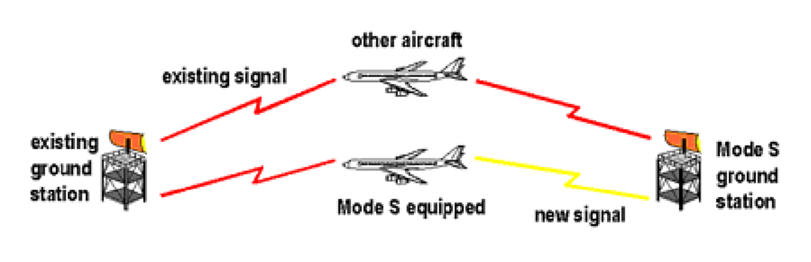
\includegraphics[width=0.80\textwidth]{Figures/modes.png}
  \caption[Interoperability: SSR and Mode S \citep{Chang2000}]{Interoperability: SSR and Mode S \citep{Chang2000}}
  \label{fig:modesinter}
\end{figure}

To use discrete addressing, each airplane has a unique identification code which is present in interrogations targeted for that airplane. Messages with a different identification code are ignored, only replying when the codes match.\\
Although the technology for Mode S was ready to use in 1975, it was not adopted immediately due to problems with manufacturing companies, which insisted in changing the initial design that made it malfunction or lack desired functions \citep{Chang2000}.\\
In 1978, a Pacific Southwest Airlines Boeing 727 collided with a private Cessna 172 during approach to Lindbergh Field in San Diego, California. The accident report states that, although the San Diego Approach Control had the capability to provide either vertical or lateral separation between IFR aircraft and participating VFR aircraft, the controller chose to give PSA 727 a visual separation clearance. This clearance gives the pilot exclusive responsibility of staying clear of other aircraft. Although the PSA pilots lost sight of the intruder Cessna, they trusted that the controller was still helping them maintaining separation and did not take timely measures to evade the aircraft which was now directly in front and below them. The following collision over a residential area resulted in the death of 137 people \citep{NationalTransportationSafetyBoard}.\\
%------TCAS------%
After this accident, the FAA increased the efforts to complete the development of an effective on-board collision avoidance system \citep{FederalAviationAdministration2011}. In 1981, FAA modified the BCAS design and created the Traffic Alert and Collision Avoidance System (TCAS), known as Airborne Collision Avoidance System (ACAS) outside the USA.\\
TCAS is an instrument integrated into other systems inside an aircraft cockpit. It is independent of the ATC ground systems, interrogating nearby ICAO compliant transponders \citep{Chang2000}. The reply contains information about range, bearing and altitude data which is used to predict collisions, prompting pilots to start evasive maneuvers \citep{FederalAviationAdministration2011}. With this, TCAS is able to help pilots with see and avoid: "TCAS functions as "electronic eyes" for pilots, providing them with an enhanced view of nearby flight traffic" \citep{MariaS.Lee2009}. \\
TCAS has two levels of sophistication: TCAS I and II. The simpler and more inexpensive TCAS I only alerts the pilot when other aircraft are close. TCAS II also provides resolutions advisories \citep{NationalTransportationSafetyBoard1986}.\\
In order to minimize the frequency of false alarms, the development of TCAS' algorithms meant the completion of several computer simulations, pilot in the loop simulations as well as testing prototype equipment on-board FAA aircraft \citep{FederalAviationAdministration2011}, which took several years to complete.\\

Meanwhile, in 1986, another mid-air collision forces changes in aviation. An Aerom\'{e}xico DC-9 collided with a private Piper PA-28-181 Archer, while approaching Los Angeles International Airport. The accident killed everybody on-board both aircraft and 15 people on the ground. During investigation, it was found that the Piper entered the Los Angeles Terminal Control Area airspace without the required clearance and that it was only equipped with a Mode-A transponder, which prevented the ATC from seeing its altitude \citep{NationalTransportationSafetyBoard1986}. Even so, both aircraft were flying in visual flight conditions and were responsible to see and avoid each other, which neither did.\\
Following this accident, the USA Congress passed the Airport and Airway Safety and Capacity Expansion Act in 1987, requiring that all carrier aircraft operating within US airspace with more than 30 passenger seats would have to be equipped with TCAS II by 1993. Aircraft with 10 to 30 seats were only required to be equipped with TCAS I \citep{SenateandHouseofRepresentativesoftheUnitedStatesofAmericainCongress1987}.\\
In Europe, EUROCONTROL defined the beginning of the year 2000 as the limit for all civil fixed-wing turbine-powered aircraft with a maximum take-off mass exceeding 15000 kg, or a maximum number of passengers of more than 30, to be equipped with TCAS II Version 7.0 and January 1st, 2005, for all civil fixed-wing, turbine-powered aircraft having a maximum take-off mass exceeding 5700 kg, or a maximum number of passengers of more than 19, to be equipped with TCAS II, Version 7.0 \citep{FederalAviationAdministration2011}.\\
ICAO would later require the implementation of TCAS II from January 1st, 2003 for all turbine-engine airplanes with a maximum take-off mass exceeding 15000 kg, or a maximum number of passengers of more than 30, and from 1 January 2005 for aircraft with more than 5700 kg or 19 passengers. ICAO also recommends that all aircraft should be equipped with a TCAS II \citep{Icao2006}.\\
%------ADS-B------%
In 1996, to avoid FAA expenditures in operating, maintaining and replenishing the old radar surveillance infrastructure, the FAA published the Surveillance Vision Plan (SVP). The SVP describes the FAA's next aircraft surveillance system, presenting a plan for its implementation in 5-year segments through 2015. It "describes the transition from ground-based radar surveillance to a joint satellite-based and ground-based surveillance system" \citep{FAA1996}.\\
The cornerstone for the new aircraft surveillance system is a collaborative system, the Automatic Dependent Surveillance-Broadcast (ADS-B). ADS-B is a technique where the aircraft position is obtained by an on-board global navigation satellite system (GNSS) receiver and then its identity, altitude and position are broadcast directly to the ground and nearby aircraft, without using satellites. It is a system similar to TCAS but ADS-B extends the same techniques to ground-based surveillance over great ranges.\\
In the USA, aircraft will only be required to operate with ADS-B after January 1st, 2020. Until then, the FAA is broadcasting traffic, weather and aeronautical information to already equipped aircraft at no cost, to motivate aircraft owners to update their systems \citep{FederalAviationAdministration2015a}.\\
In Europe, all aircraft with maximum take-off mass greater than 5700 kg or maximum cruising True Air Speed greater than 250 kts have to be equipped with ADS-B, after 8 June 2016 for forward fit and June 7th, 2020, for retrofit \citep{TheEuropeanCommission2014} \: \citep{TheEuropeanCommission2011}.

\subsection{See and Avoid in General Aviation}
\label{subsection:gat}
In the general aviation, there are several technologies that complement the practice of see and avoid. The most important are discussed bellow.

\subsubsection{Position and Anti-Collision Lights}
\label{subsubsection:poslights}
One of the first systems created to help see and avoid were the Position Lights. 
Based on the system used in maritime navigation, it evolved into what is used today, showed in \ref{fig:navlights1}.

\begin{figure}[!htb]
  \centering
  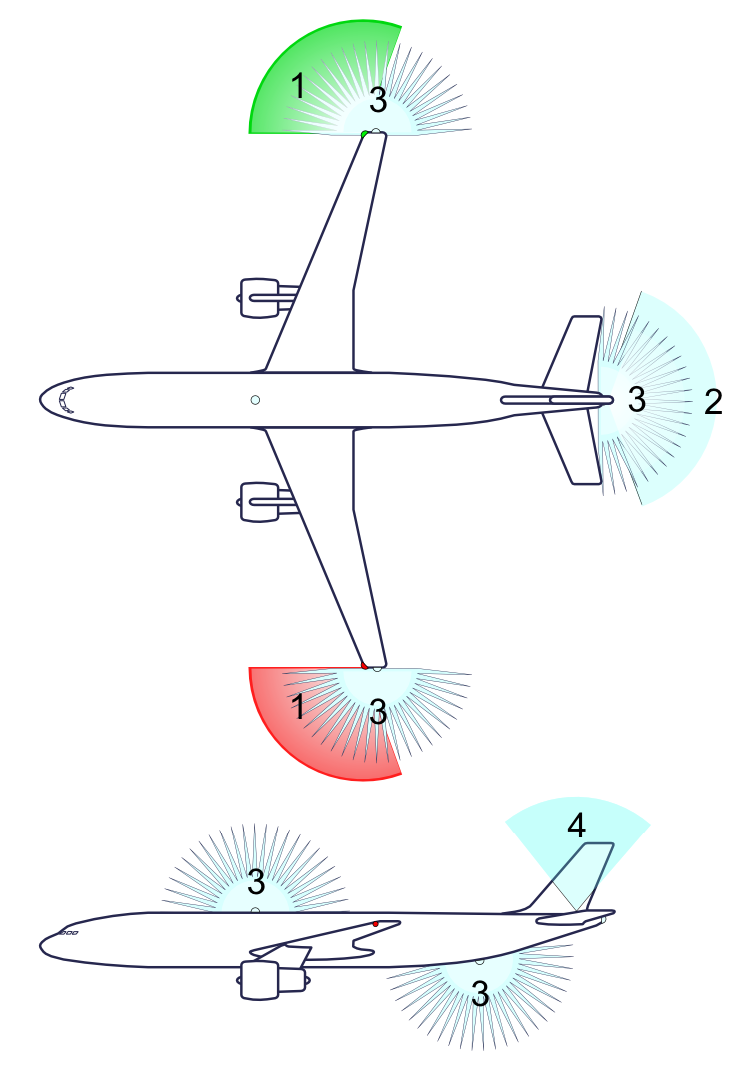
\includegraphics[width=0.35\textwidth]{Figures/navigationlights.png}
  \caption[Aviation Lights used in See and Avoid \citep{Tosaka2010}]{Aviation Lights used in See and Avoid. 1) Left and Right Position Lights; 2) Rear Position Light; 3) Anti-collision Lights; 4) Logo Light; \citep{Tosaka2010}}
  \label{fig:navlights1}
\end{figure}

The position lights must be turned on from sunset to sunrise for aircraft operated on the surface and in flight. The Anti-Collision lights must be on during all operations, day or night, except when they may constitute a hazard to safety during adverse meteorological conditions \citep{FederalAviationAdministration2015a}.\\
The position lights system must be composed by a red light on the left side and a green light on the right side, spaced as far as practicable, and a white light mounted as far back as possible (on the tail or each wing tip) \citep{Easa2012}.
The left (L) and right (R) position lights' dihedral angles are formed by two intersecting vertical planes, one parallel to the longitudinal axis of the aircraft and a second at 110\degree to the left and the right, respectively, as viewed when looking from the back to the front of the airplane \citep{Easa2012}. 
The rear (A) position light dihedral angle is formed by two intersecting vertical planes, each making a 70\degree angle to the right and to the left to a vertical plane parallel to the longitudinal axis \citep{Easa2012}. \\
In the horizontal plane, the position lights have the intensity requirements in \ref{tab:inthor}. For any vertical planes, the requirements depend on the horizontal plane minimum intensity I, and gradually decrease until a minimum is reached at 90\degree .\\

\begin{table}[!htb]
\begin{center}
\caption[Minimum intensities in the horizontal plane for position lights \citep{Easa2012}]{Minimum intensities in the horizontal plane for position lights \citep{Easa2012}.}
\begin{tabular}{ccccc}
Light Position & \multicolumn{3}{c}{Left and Right} & Rear \\ 
\hline 
Angle measured from dead ahead & 0\degree to 10\degree & 10\degree to 20\degree & 20\degree to 110\degree & 110\degree to 180\degree \\ 
Intensity (candelas) & 40 & 30 & 5 & 20 \\ 
\end{tabular}
\end{center}
\label{tab:inthor}
\end{table}

The position lights also have maximum intensities in overlapping beams of position lights \citep{Easa2012}.\\

For the anti-collision light system, an aircraft must have one or more approved aviation red or aviation white anti-collision lights located in a place that will not diminish the pilot's vision and the position lights visibility. These lights must have a field of coverage greater than or equal to 75\degree bellow and above the horizontal plane with no more than 0.5 steradians of obstructed visibility \citep{Easa2012}. They should also have a flash frequency between 40 and 100 cycles per minute, and between 40 and 180 in any overlaps when the system has more than one light.
Each anti-collision light must have an effective intensity which depend on the duration of the blink \citep{Easa2012}.

\subsubsection{Mode S}
\label{subsubsection:modes}

Mode S was designed to solve several faults in the previous Modes A and C. 

While addressing the problems with interference generated with the increasing amount of replies in the communication channels already approached in \ref{subsection:evolution}, mode S was designed as a discrete addressing system. This means that each aircraft's transponder has a unique identification code and will not answer to interrogations containing a different one.

As discussed in section \ref{subsection:evolution}, one of the requirements for Mode S was the interoperability with older modes, which meant that the new technology must be retro-compatible and transparent. \\
In order to achieve retro-compatibility, the same frequencies (1030 MHz uplink and 1090 MHz downlink) are used in Mode S. This allows new Mode S equipment to receive and interpret signals from SSR. On the other hand, the use of the same frequencies makes it harder for the new Mode S signal not to interfere with previous system's transponders and ground stations (transparency). This problem was solved using the sidelobe suppression technique used in the SSR which consisted in the comparison of two pulses P1 and P2 \citep{Chang2000}. SSR equipment was able to compare the signal (P1) from the main directional antenna with the signal (P2) transmitted by an omnidirectional antenna immediately after P1. P2 is weaker in the direction of the main lobe of P1, but stronger otherwise, as can be seen in figure \ref{fig:suppression}. If an aircraft was located inside P1 main lobe, like aircraft 1, it would receive a much stronger P1 pulse than P2, and a stronger P2 otherwise, as can be seen in figure \ref{fig:suppressionpulses}. SSR transponders only answer in positions where P1 pulse is stronger than P2, like aircraft 1. When located in other places, the transponder would be temporarily disabled for 35 microseconds \citep{Chang2000}.

\begin{figure}[!htb]
  \centering
  \includegraphics[width=0.35\textwidth]{Figures/suppression.png}
  \caption[ATCRBS Broadcast with Omnidirectional Antenna \citep{Chang2000}]{ATCRBS Broadcast with Omnidirectional Antenna \citep{Chang2000}}
  \label{fig:suppression}
\end{figure}

\begin{figure}[!htb]
  \centering
  \includegraphics[width=0.35\textwidth]{Figures/suppressionpulses.png}
  \caption[ATCRBS Broadcast Pulses \citep{Chang2000}]{ATCRBS Broadcast Pulses (A1 - aircraft 1; A2 - aircraft 2) \citep{Chang2000}}
  \label{fig:suppressionpulses}
\end{figure}

To enable transparent operation, mode S was designed to use this technique: its signal begins with two pulses similar to the one received by an aircraft on the sidelobe of an SSR ground station. After receiving this signal, SSR equipment will be disabled for 35 microseconds and only mode S equipment will receive the remaining signal.\\
The shape of mode S signal can be seen in figure \ref{fig:suppressionmodes}. Because mode S can only transmit while SSR equipment is disabled, the transmitted message was restricted to a length of 112 bits \citep{Chang2000}.\\

\begin{figure}[!htb]
  \centering
  \includegraphics[width=0.50\textwidth]{Figures/suppressionmodes.png}
  \caption[Mode S Signal with Sidelobe Suppression \citep{Chang2000}]{Mode S Signal with Sidelobe Suppression \citep{Chang2000}}
  \label{fig:suppressionmodes}
\end{figure}

Mode S introduced "the technical base for a digital communication exchange system" \citep{OfficeofTechnologyAssessment1980}. This capacity would bring an increase in the development of several services that, using the digital link, would be inexpensive to implement and use, like the Traffic Information Service, the Graphical Weather Service and TCAS.

\subsubsection{ACAS}
\label{subsubsection:tcas}
The Airborne Collision Avoidance System (ACAS) was introduced to reduce the risk of mid-air collisions, by providing pilots advice through resolution advisories (RAs) and traffic advisories (TAs). RAs are maneuvers recommended to the pilot to avoid an intruder aircraft, while TAs help the pilot visually acquire the position of the intruder.\\
ACAS was designed as a back-up for the ATC system and is not dependent on ground-based systems \citep{Icao2006}. By interrogating Mode A/C and Mode S transponders on nearby aircraft and processing their replies, ACAS is able to determine potential collision threats and provide the appropriate advisories to avoid them \citep{Eurocontrol2010}, with three different levels of capability:
\begin{itemize}
\item ACAS I provides information to aid "see and avoid" and does not provide RAs. It is usually installed on rotorcraft and small fixed-wing aircraft \citep{Icao2006}.
\item ACAS II provides TAs and RAs with vertical maneuvers to increase or maintain the vertical separation from an intruder aircraft. It was designed to be installed on fixed-wing aircraft \citep{Icao2006}. 
\item ACAS III is a system that provides RAs using vertical and horizontal maneuvers to increase or maintain the existing separation. There are no ACAS III implementations to date \citep{Eurocontrol2010}.\\
\end{itemize}
As an implementation of ACAS III is not expected due to difficulties with horizontal tracking \citep{Eurocontrol2015}, there is research being conducted to develop the next version of ACAS, ACAS X, which will use dynamic programming to optimize the generation of RAs \citep{Eurocontrol2015}.
As the only fully compliant implementation of ACAS I and II, to date, is the Traffic alert and Collision Avoidance System (TCAS) I and II, respectively, the terms ACAS and TCAS can be used interchangeably \citep{Eurocontrol2015}.\\
The level of protection given by TCAS depends on the equipment inside the target aircraft, as can be seen in table \ref{tab:tcasprotec}. If the target aircraft does not have an operating transponder, TCAS cannot provide any protection \citep{FederalAviationAdministration2011}.\\

\begin{table}[!htb]
\begin{center}
\caption[TCAS Levels of Protection \citep{FederalAviationAdministration2011}]{TCAS Levels of Protection \citep{FederalAviationAdministration2011}.}
\begin{tabular}{cccc}
                                           &                      & \multicolumn{2}{|c}{Own Aircraft Equipment}                  \\
                                           & \multicolumn{1}{l}{} & \multicolumn{1}{|c}{TCAS I} & \multicolumn{1}{c}{TCAS II}    \\ \hline
\multirow{4}{*}{Target Aircraft Equipment} & \multicolumn{1}{c|}{Mode A}              & TA                         & TA                             \\
                                           & \multicolumn{1}{c|}{Mode C or Mode S}    & TA                         & TA and Vertical RA             \\
                                           & \multicolumn{1}{c|}{TCAS I}              & TA                         & TA and Vertical RA             \\
                                           & \multicolumn{1}{c|}{TCAS II}             & TA                         & TA and Coordinated Vertical RA \\ \hline
\end{tabular}
\end{center}
\label{tab:tcasprotec}
\end{table}

When a target aircraft is in range and after several consecutive replies received from its transponder, TCAS divides the range with the closure rate, calculating the time, also known as \textit{tau}, until the Closest Point of Approach (CPA). After this, depending on the type of TCAS, it can issue the already mentioned TAs and RAs. Traffic Advisories will always be issued first, to help the pilot detect the target or to prepare him for an RA (only in TCAS II), when the \textit{tau} is bellow 20 or 48 seconds (with own altitude $<$1000 ft or $>$42000 ft respectively). If the aircraft is equipped with TCAS II, an RA will be issued, when the \textit{tau} is bellow 15 seconds for an altitude between 1000 ft and 2350 ft, and 35 seconds for an altitude greater than 42000 ft, containing recommended maneuvers. The \textit{tau} defines the protection volume given by TCAS, as shown in figure \ref{fig:tcasvolume}. If the target aircraft is also equipped with TCAS II, the RAs will be automatically coordinated through Mode S communications \citep{FederalAviationAdministration2011}.\\

\begin{figure}[!htb]
  \centering
  \includegraphics[width=0.90\textwidth]{Figures/tcasvolume.png}
  \caption[TCAS Protection Volume \citep{FederalAviationAdministration2011}]{TCAS Protection Volume - Not to scale \citep{FederalAviationAdministration2011}}
  \label{fig:tcasvolume}
\end{figure}

In order to have a fully functional TCAS II, an aircraft needs to have several components, as shown in figure \ref{fig:tcashardware}.\\

\begin{figure}[!htb]
  \centering
  \includegraphics[width=0.90\textwidth]{Figures/TCAShardware.png}
  \caption[Block diagram of TCAS and transponder hardware components required for standard TCAS equipment \citep{QinetiQ2013}]{Block diagram of TCAS and transponder hardware components required for standard TCAS equipment \citep{QinetiQ2013}}
  \label{fig:tcashardware}
\end{figure}

The TCAS II Processor uses data from several sensors, like radar altimeter, to monitor the aircraft state. At the same time, it performs airspace surveillance and intruder tracking simultaneously, using the Mode S Transponder to coordinate complementary RAs, when required, via the provided air-to-air data exchange protocol already mentioned in chapter \ref{subsubsection:modes}.
The TCAS and SSR control panel is the platform that allows the flight crew to control all TCAS equipment, including the Mode S transponder. It usually provides four different control positions \citep{FederalAviationAdministration2011}: 
\begin{itemize}
\item Standby - TCAS does not issue interrogations, Mode S Transponder replies only to discrete interrogations.
\item Transponder - Mode S Transponder operational, replying to all appropriate ground and TCAS interrogations. TCAS in standby.
\item TA Only - Mode S Transponder operational. TCAS operational but will only issue TAs.
\item Automatic - Mode S Transponder operational. TCAS operational, issuing the appropriate TAs and RAs.
\end{itemize}

In order to provide airspace surveillance and track intruders, TCAS needs several antennas, including a top directional antenna and a bottom antenna.  The antennas transmit interrogations at 1030 MHz and receive replies at 1090 MHz. The system may share these antennas with the Mode S transponder or have separate ones \citep{FederalAviationAdministration2011}.\\
Finally, the system uses both visual and aural signals to present the information to the flight crew, using predefined symbols and words.\\

Although TCAS is being tested for UAS use, it cannot be directly installed on an unmanned aircraft, as it was not designed for that purpose \citep{Icao2006}, but only for aircraft with an on-board pilot which is responsible for evaluating all the available information and decide to follow the RA or not. Adding to this, TCAS II was developed for fixed-wing aircraft and not for the different configurations available for unmanned aircraft which present different performance spectrum that may be outside the one required for response times, vertical accelerations and vertical rates in TCAS II \citep{Eurocontrol2010}.
Due to the amount of required equipment, TCAS is nowadays too large, heavy, power consuming \citep{Elliott2012} \citep{FederalAviationAdministration2015} and prohibitively expansive for small UAS operations, with the TCAS I equipment price above \$ 25,000 \citep{Smith2005}. Finally, TCAS can only reliably provide surveillance with traffic densities lower than or equal to 0.3 aircraft per square nautical mile (24 aircraft within 5 nmi radius) \citep{FederalAviationAdministration2011}, which may not be enough for the desired operation.
 

\subsubsection{ADS-B}
\label{subsubsection:adsb}

As mentioned in \ref{subsection:evolution}, the Automatic Dependent Surveillance-Broadcast (ADS-B) is a technique that, using the position obtained by an on-board GNSS receiver, broadcasts (ADS-B Out) the aircraft's state vector (3D position and 3D velocity) for ground-based and aircraft-based surveillance \citep{Lester2007} \citep{Costin2012}, as can be seen in figure \ref{fig:adsbscheme}.

\begin{figure}[!htb]
  \centering
  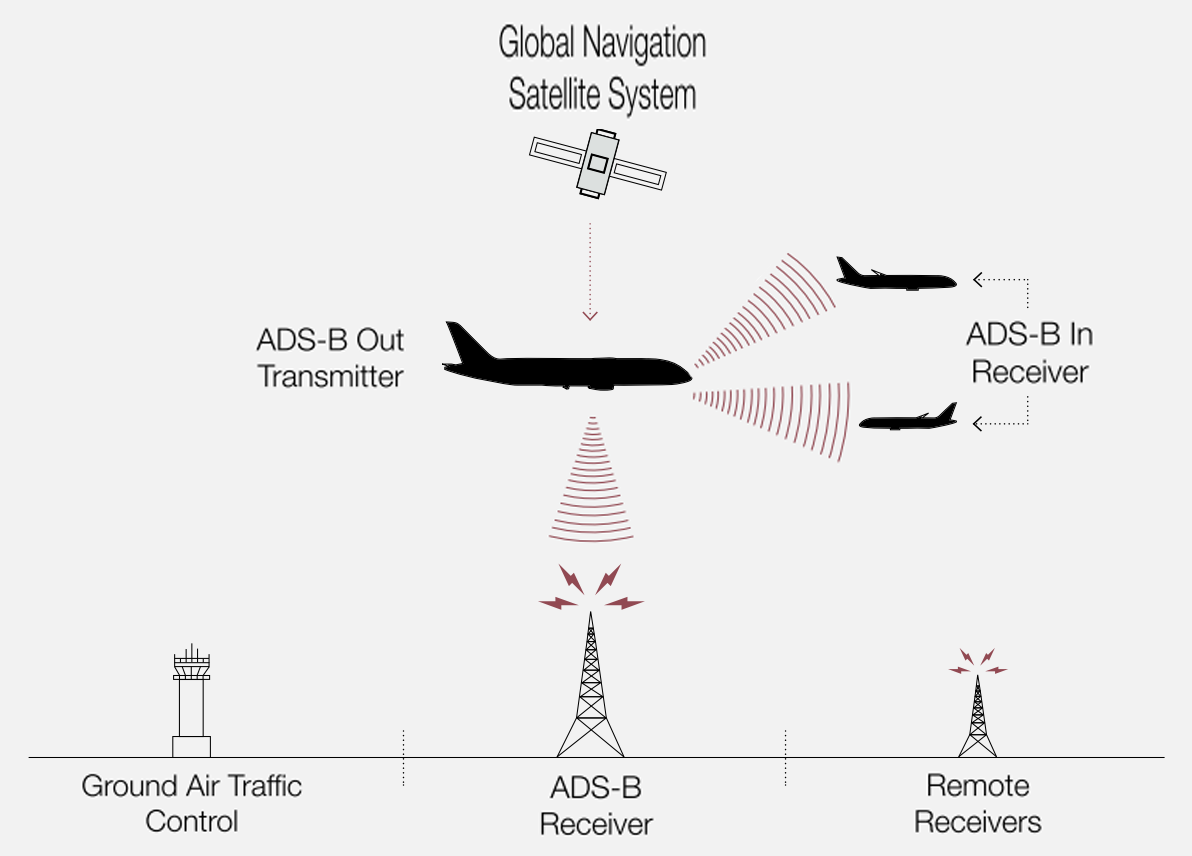
\includegraphics[width=0.90\textwidth]{Figures/ADS-B2.png}%ADS-B1.jpg}
  \caption[ADS-B communications \citep{Richards2010}]{ADS-B communications \citep{Richards2010}}%%\citep{Allen2012}}
  \label{fig:adsbscheme}
\end{figure}

By providing this information to nearby aircraft (ADS-B In), the pilots can perform collision avoidance without instructions from the ATC \citep{Lester2007} \citep{Costin2012}. With the received state vector and its own, the aircraft is able to calculate relative range and bearing to the transmitting aircraft and display this information to the pilot on a Cockpit Display of Traffic Information (CDTI). 

ADS-B, as a broadcast technology, does not require any replies. The aircraft is always broadcasting it's state vector unlike TCAS, which only sends information when interrogated. Since it does not require any action from the pilot, it is automatic. Finally, as it depends on the aircraft to acquire its position and its transmitter to broadcast the signal, it is considered as dependent surveillance.

There are several data links to enable ADS-B communication: Mode S 1090 MHz Extended Squitter (1090-ES), Universal Access Transceiver (UAT) operating at 978MHz and VDL (VHF Digital Link) Mode 4. The FAA has only approved the first two, while EUROCONTROL only accepts 1090-ES.

1090-ES is an update to Mode S, mentioned in subsection \ref{subsubsection:modes}.  When equipped with this version of Mode S transponder, an aircraft transmits the additional data required for ADS-B Out, without interrogations from TCAS or SSRs.

UAT is a data link used for wideband broadcast operating on 978MHz that has a modulation rate of 1.042 Mbps \citep{ACP2005}. It was designed for ADS-B communications but it also supports other related services, like Flight Information Service - Broadcast (FIS-B) and Traffic Information Service - Broadcast (TIS-B). Although it was initially thought to be the most probable protocol to be adopted for ADS-B, it hasn't been accepted internationally because it operates in frequencies close to some DME stations \citep{Lester2007}.  

Finally, VDL Mode 4 is a protocol designed by a Russian-Swedish cooperation. It operates in 108-137 MHz range, using 25kHz communication channels and has a modulation rate of 0.0315 Mbps with a D8PSK modulation scheme or 0.0192 Mbps with a Gaussian-filtered Frequency Shift Keying \citep{proesch2015}. It supports both communications data link and surveillance data link. It was rejected in the USA due to its high implementation cost as well as the lack of ICAO assigned frequencies at the time \citep{Lester2007}.

Although the ADS-B out technology offers a better solution for collision avoidance than TCAS, the upgrade may have high costs for operators. Depending on the required ADS-B standard, the operator may have to upgrade to a wide area augmentation system (WAAS) certified GNSS receiver and/or a new flight management system (FMS) computer \citep{Lester2007}.

\section{New developments on SAA}
\label{section:newsaa}
With the increase of UA use, the problem of operations in the same airspace as manned aircraft has to be dealt with.
There are already several proposals and guides to regulate this problem, but only some countries have defined requirements and laws that regulate UA's use.\\
In Europe, although EUROCONTROL has published no legislation for UA under 150 kg, several European countries have their own requirements. The United Kingdom released on 29 May 2002 the Civil Aviation Publication 722 - Unmanned Aircraft System Operations in UK Airspace - Guidance, which was last updated on 24 March 2015. This document provides guidance for UK unmanned aircraft users.\\
In the United States of America, the FAA has proposed regulation for Unmanned Aircraft Systems on the first trimester of the year 2015.\\
Until now, all the existing legislation is only allowing operations in segregated airspace due to, as mentioned in \ref{section:saa}, the impossibility of using see and avoid without a pilot on-board. In order to enable operations in non-segregated airspace, an SAA solution that can provide the required separation must be created \citep{FederalAviationAdministration2015}.\\
Multiple authorities state that UA must provide at least the same reliability as manned aircraft to operate in the same airspace \citep{InternationalCivilAviationOrganization2011}. In order to achieve the required reliability, UA would have to use high reliability components or increase hardware redundancy \citep{Angelov2012}, like the general aviation. Due to limits in sUA payload dimensions and weight as well as the cost benefit of the activities where sUA may be involved, both options may not be easy to implement: higher reliability components are more expensive than the equipment being used now and it is almost impossible to increase the hardware redundancy without exceeding the aircraft maximum payload. These limitations create a problem with the kind of payload that might be used for SAA.\\
As mentioned in section \ref{subsubsection:tcas}, TCAS and ADS-B both require equipment that is not appropriate for sUA \citep{FederalAviationAdministration2015}. Although ADS-B's use in GA is growing, the required (certified) GNSS equipment represents a cost that most sUA users cannot afford. By using non-certified equipment, the obtained position has a much higher position error and there is no error estimation provided. Adding to this, the required transmitting equipment for both ADS-B and TCAS is still too large, heavy and power consuming for an appropriate range.\\
A possible solution is to lower the requirements for small UA's SAA reliability proportionally to their size, weight and velocity.\\
Another step to enable UA operations in unsegregated airspace, is to develop and mandate a short-range, low power and lightweight cooperative technology for collision avoidance first and a non-cooperative later, as the development of a technology that enables the detection of non-cooperative aircraft may cost US\$ 2 billion and take several more years \citep{Angelov2012}.\\

\section{SAA development programs}
\label{section:saaprograms}
Due to the increasing availability and disseminated use of UA, the risk of a collision is increasing. In an attempt to prevent this, there are already several programs worldwide studying sense and avoid. Some of them are presented bellow.\\
\subsection{MIDCAS}
The Mid Air Collision Avoidance System Project is an european industrial consortium composed by: SAAB, Alenia Aeronautica, CIRA (Italian Aerospace Research Center), Diehl BGT Defence, DLR (German Aerospace Center), Airbus Defense and Space, ESG Elektroniksystem- und Logistik-GmbH, Indra, Sagem, Selex ES and Thales. It was launched in 2009 by five member states (France, Germany, Italy, Spain and Sweden) under the framework of the European Defence Agency with three main focus \citep{Consortium2011}:
\begin{itemize}
\item Progress on Standards for SAA.
\item Design of a generic SAA function to be tested in simulations.
\item Design of an SAA Demonstrator to be tested in manned and Remotely Piloted Aircraft Systems (RPAS) flight.
\end{itemize}
Their aim is to contribute to the RPAS integration in civilian airspace by proposing a baseline of solutions for the "Unmanned Aircraft System Mid-air Collision Avoidance Function" acceptable by the manned aviation.\\
Flights tests with Alenia Aeronautica's Sky-Y with a payload of SAA cooperative and non-cooperative sensors, as can be seen in figure \ref{fig:midcas}, were performed in Italy between December 2014 and April 2015. During this time, the UA was able to perform fully automated avoidance maneuvers to avoid collision with a manned aircraft.

\begin{figure}[!htb]
  \centering
  \includegraphics[width=0.90\textwidth]{Figures/midcas.jpg}
  \caption[Sense and Avoid Demonstrator \citep{EuropeanDefenceAgency2015}]{Sense and Avoid Demonstrator \citep{EuropeanDefenceAgency2015}}
  \label{fig:midcas}
\end{figure}
	
\subsection{UAS Integration in the NAS Project}
The UAS Integration in the National Airspace System (NAS) Project is the FAA's attempt to integrate unmanned aircraft into the NAS "without reducing existing capacity, decreasing safety, negatively impacting current operators, or increasing the risk to airspace users or persons and property on the ground any more than the integration of comparable new and novel technologies" \citep{FederalAviationAdministration2013}.
Its goal is to reduce technical barriers associated with integrating UAS into the NAS utilizing integrated system level tests in a relevant environment \citep{Rugg2015}.\\
In 2013, the project published the Integration of Civil Unmanned Aircraft Systems (UAS) in the NAS Roadmap, with the purpose of outlining, "within a broad timeline, the tasks and considerations needed to enable UAS integration into the National Airspace System (NAS) for the planning purposes of the broader UAS community" \citep{FederalAviationAdministration2013}. This roadmap defines a 5 year near term, 5 to 10 mid-term and a longer than 10 years long-term with plans and expected results for each period. All three terms try to harmonize with the international community and several segments of society (industry, civil liberties and national security), namely with ICAO, following the considerations on the Circular 328 "Unmanned Aircraft Systems (UAS) Circular". This circular provides guidelines for Member States to integrate UAS into their airspace in a consistent manner, so that global compatibility may be achieved when possible.\\
%To help the FAA in the integration of the UAS in the NAS, the RTCA formed the Special Committee 203 (SC-203) in 2004. The SC-203 developed and published several guidelines for UAS integration \citep{FederalAviationAdministration2013}:
%\begin{itemize}
%\item UAS must operate safely, efficiently, and compatibly with service providers and other users of the NAS so that overall safety is not degraded;
%\item UAS will have access to the NAS, provided they have appropriate equipage and the ability to meet the requirements for flying in various classes of airspace;
%\item Routine UAS operations will not require the creation of new special use airspace, or modification of existing special use airspace;
%\item Except for some special cases, such as small UAS (sUAS) with very limited operational range, all UAS will require design and airworthiness certification to fly civil operations in the NAS;
%\item UAS pilots will require certification, though some of the requirements may differ from manned aviation;
%\item UAS will comply with ATC instructions, clearances, and procedures when receiving air traffic services; 
%\item UAS pilots (the pilot-in-command) will always have responsibility for the unmanned aircraft while it is operating;
%\item And UAS commercial operations will need to apply the operational control concept as appropriate for the type of operation, but with different functions applicable to UAS operations.
%\end{itemize}
%Meanwhile, the FAA has established several UAS test sites to help them gain a better understanding of operational issues. Although privacy policies are not part of the FAA mission, any one operating at these test sites will have to develop a privacy policy. The developed privacy policies will help "inform the dialogue among policymakers, privacy advocates, and the industry regarding broader questions concerning the use of UAS technologies in the NAS" \citep{FederalAviationAdministration2013}.\\

\subsection{Geyer's prototype SAA system}
Carnegie Melon University's investigators approached SAA using vision systems, avoiding cooperative communication systems \citep{Geyer2008} \citep{Geyer2009} \citep{Dey2010}. To determine the minimum requirements of the sense component, they first developed the collision avoidance component and computed its maximum performance.\\
Their work was divided into the following tasks \citep{Geyer2009}:
\begin{itemize}
\item Task 1: develop an aircraft detection and collision warning system prototype.
\item Task 2: develop a collision avoidance system prototype.
\item Task 3: investigate alternative technologies.
\end{itemize}

It was found that the performance factors for an SAA system that uses vision can either be controllable or not, as showed in figure \ref{fig:geyer1}.
\begin{figure}[!htb]
  \centering
  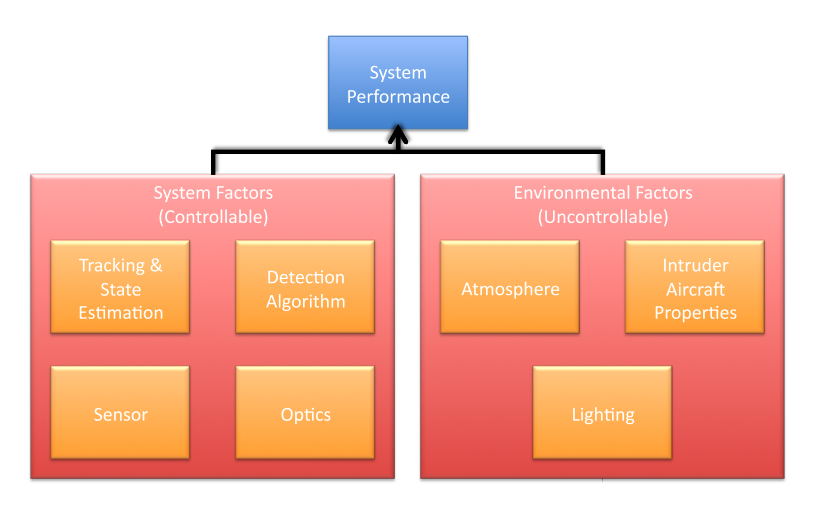
\includegraphics[width=0.90\textwidth]{Figures/Geyer1.png}
  \caption[Geyer's diagram of factors determining the performance of an aircraft detection system \citep{Geyer2009}]{Geyer's diagram of factors determining the performance of an aircraft detection system \citep{Geyer2009}}
  \label{fig:geyer1}
\end{figure}

When developing their system, they assume that the environmental factors are no worse than the limits of VMC (visual meteorological conditions).\\
During their tests, the investigators obtained a detection rate of over 99\% for a range of 3 miles, with one false positive every 20 frames with a IPX-4M15 camera and Zeiss 85 mm lens. For 5 miles, with the same false positive per frame and camera, detection rate of 98.1\%. Most false positives were birds or ground landmarks.\\
Their prototype was able to compute an avoidance maneuver within 500 ms as long as the intruder was at least 2.1 km away, flying at no more than 250 knots, making maneuvers that did not exceed 1G, and the detecting aircraft was traveling at, at least, 40 knots.\\
The major problems found with the approach used were the following:
\begin{itemize}
\item Difficult to determine if intruder is in collision course or not. 
\item Hard to detect bellow horizon due to ground noise.
\item May require image processing specialized hardware for image processing.
\item Difficult to include right-of-way rules, as it is hard to identify the intruder.
\end{itemize}

\subsection{ASTRAEA}
The Autonomous Systems Technology Related Airborne Evaluation \& Assessment (ASTRAEA) is a UK industry-led consortium composed by seven companies (Airbus Defence \& Space, AOS, BAE Systems, Cobham, QinetiQ, Rolls-Royce and Thales) founded in 2006 which seeks to find solutions that enable the integration of UAS into the UK airspace \citep{Ansell2011}. Their objectives are \citep{Dopping-Hepenstal2012}:
\begin{itemize}
\item Enable the routine use of UAS in all classes of airspace without the need for restrictive or special conditions of operation.
\item Develop and demonstrate key technologies and operating procedures required to open up the airspace.
\item Support the development of the regulatory framework for this new class of operation.
\end{itemize}
Since it was founded, the ASTRAEA was able to developed a complex flight management system, the Autonomous Integrated Mission System (AIMS) which is an independent core avionic system and contains, among others, air collision avoidance, adaptive and variable autonomous decision making to decrease pilot workload and loss of communications and on-board system health management. 

\subsection{Nussberger's Aerial Object Tracking from an Airborne Platform}

A team of investigators from The Computer Vision Laboratory, ETH Zurich, developed an experimental Sense and Avoid system integrated into an aircraft to detect and track other aerial objects with electro-optical sensors \citep{Nussberger2014}.\\
To test the developed system, data of real aircraft was obtained by implementing the system on a Diamond DA42 aircraft (manned aircraft). The implemented system was composed by a data logger in the back of the aircraft and several sensors on the aircraft nose, such as ADS-B receiver for cooperative traffic and two cameras to detect non-cooperative traffic. All these sensors produced about 300 MB/s of data continuously which was processed by a custom logging software, so as to provide accurate time handling between the several sources.\\
Tests were performed during daytime, where more than 5 hours of video and meta-data from the different sensors were obtained in 40 different scenarios \citep{Nussberger2014}. The ground truth of the intruder was recorded using a differential GPS.\\
The system provided an average time to collision for having a valid track between 15 and 20 seconds, with a corresponding distance greater than 1500m. Results were worse for head-on scenarios which provide a lower visible cross-section of the intruder and a higher closing speed, when the sun was closer to the horizon and when the weather conditions deteriorated.

\section{Existing equipment}
\label{section:existingequipment}
There are already several companies producing technology that enables or helps the regulation of UA operation. Some examples are presented below.
\subsection*{Exelis' Symphony} 
\label{subsection:symphony}
Symphony is a system that fuses data from multiple sources, such as ADS-B ground stations and primary and secondary radar, to provide a broad picture of the airspace's traffic through web-based solutions \citep{Exelis2011}, as can be seen in figure \ref{fig:symphony}. The possibility of including UA data, either by the already used technologies such as ADS-B or by accessing information the operator obtains from data-link, is being investigated \citep{GrahamWarmick2015}.

\begin{figure}[!htb]
  \centering
  \includegraphics[width=0.90\textwidth]{Figures/symphony.png}
  \caption[Symphony OpsVue example \citep{HarrisCorporation2015a}]{Symphony OpsVue view on a web browser \citep{HarrisCorporation2015a}}
  \label{fig:symphony}
\end{figure}

\subsection*{SARA's PANCAS} 
\label{subsection:pancas}
SARA's Passive Acoustic Non-cooperative Collision-Alert System (PANCAS) uses the Low Cost Scout UAV Acoustic System (LOSAS) technology, composed by four acoustic probes. It detects, locates and tracks targets as well as generates automatic collision avoidance maneuvers \citep{SARA2012}. By gathering GPS information from the flight control system, it can estimate the absolute location of the target, sending this information to the operator by data-link. The system weights 250g and consumes 7W of 6V DC power, as demonstrated in figure \ref{fig:pancas}.

\begin{figure}[!htb]
  \centering
  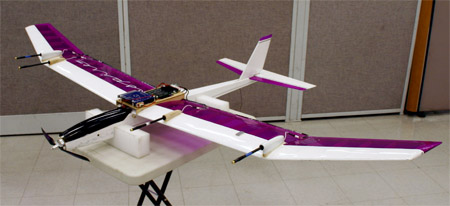
\includegraphics[width=0.75\textwidth]{Figures/Pancas.jpg}
  \caption[PANCAS demonstration aircraft \citep{SARA2012}]{PANCAS demonstration aircraft \citep{SARA2012}}
  \label{fig:pancas}
\end{figure}

\subsection*{Skyward} 
\label{subsection:skyward}

Skyward is an information management platform for commercial UA operators. They provide information to ensure safe flights and in compliance with regulations \citep{Evans2015}. The Drone Airspace Map provides situation awareness with real time area of operations, hazards, restricted zones and temporary flight restrictions, as is shown in figure \ref{fig:skyward}. The platform also allows the creation of flight plans and flight logs, which can then generate the required reports \citep{Skyward2015}.

\begin{figure}[!htb]
  \centering
  \includegraphics[width=0.90\textwidth]{Figures/skyward.png}
  \caption[Skyward example flight area map \citep{Skyward2015}]{Skyward example flight area map \citep{Skyward2015}}
  \label{fig:skyward}
\end{figure}

%\subsection*{Lockheed Martin's Flight Service Pilot Web} 
%\label{subsection:lockheedweb}
%Lockheed Martin's Flight Service Pilot Web \citep{Gibson2015}

\subsection*{AVEO's AECAS100}
\label{subsection:aecas}
The AVEO Collision Avoidance System 100 (AECAS100) is an electronic unit that receives sensor data and steering command from the autopilot or flight management unit (FMU), and provides a correction of the original command to avoid collisions \citep{AEVOGmbH2015}. The sensor data can be transmitted directly to the unit or from a processing unit. Although it can receive data from several types of sensors that use the correct communication protocol, the unit supports direct interface with both RPLidar from RoboPeak and URG-04LX-UG01 from Hokuyo (both laser scanners with maximum range of about 6m).
The AECAS 100 requires obstacle information in two dimensions, which it assumes to be in the horizontal plane, to provide roll and pitch corrections with a frequency of 20 Hz.
Each unit weights 120g and requires between 4.5 and 5.5V and 2.0A of power through a 2.1mm barrel connector, as can be seen in figure \ref{fig:aecas}.

\begin{figure}[!htb]
  \centering
  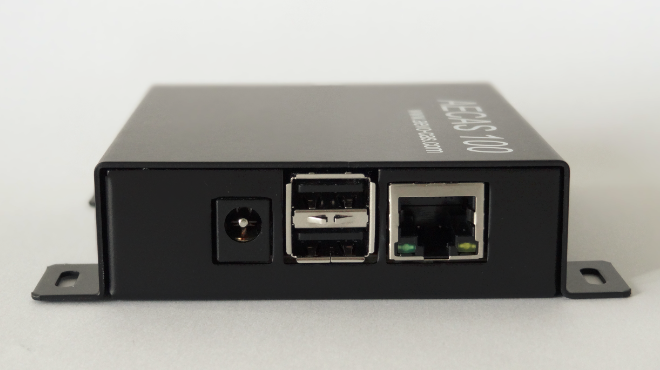
\includegraphics[width=0.6\textwidth]{Figures/aecas100.png}
  \caption[AECAS 100 unit \citep{AEVOGmbH2015a}]{AECAS 100 unit \citep{AEVOGmbH2015a}}
  \label{fig:aecas}
\end{figure}

\subsection*{DJI's guidance} 
\label{subsection:dji}
DJI's guidance is a sensor-based navigation aid \citep{DJI2015}. It uses data from several ultrasonic and image sensors to help avoid obstacles and perform hover by transmitting velocity, position and obstacle clearance to the autopilot.\\
With a weight of 279 g, it requires an input voltage between 11.1 V and 25 V, and consumes a maximum of 12 W. During operation, it requires good lighting and texture-rich surfaces with clear patterns and it is able to measure velocity until 16 m/s with an accuracy of 0.04 m/s. The sensors have a minimum effective range of 0.20 m and maximum of 20 m \citep{DJI2015}.

\begin{figure}[!htb]
  \centering
  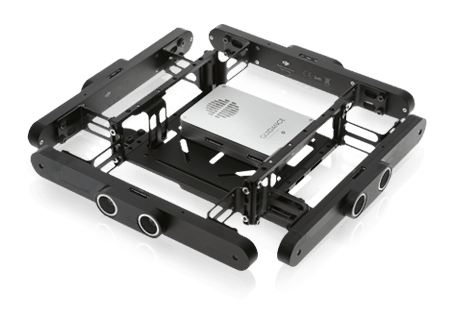
\includegraphics[width=0.6\textwidth]{Figures/guidance.png}
  \caption[DJI Guidance \citep{DJI2015a}]{DJI Guidance \citep{DJI2015a}}
  \label{fig:guidance}
\end{figure}

\subsection*{Unilight} 
\label{subsection:unilight}
Unilight is an Austrian company that manufactures small aircraft lighting. 
All lights are equipped with high performance LEDs to lower consumption and increase visibility.
To enable different behaviors for different types of lights, several controllers are also available which can be programmed according to the specific needs. Controllers range from a simple 1 channel controller, which costs \euro{24.90} and weights approximately 1.5 g without wires, to a USB programmable 8 channel controller, which costs \euro{74.90} and weights 18 g without cables \citep{Rockstroh2014}. 
The available lighting systems cover all the required aircraft lights, such as navigation lights (figure \ref{fig:unilight}) and anti-collision flashers. 
All the available controllers and lights can be directly connected to a 2S battery and come with a resistor that can be added to enable 3S batteries \citep{Mchale2015}.

\begin{figure}[!htb]
  \centering
  \includegraphics[width=0.60\textwidth]{Figures/unilight.png}
  \caption[Unilight navigation light \citep{Rockstroh2014}]{Unilight navigation light \citep{Rockstroh2014}}
  \label{fig:unilight}
\end{figure}

 % file "Thesis_StateofArt.tex"

%%%%%%%%%%%%%%%%%%%%%%%%%%%%%%%%%%%%%%%%%%%%%%%%%%%%%%%%%%%%%%%%%%%%%%%%
%                                                                      %
%     File: Thesis_VisualSolution.tex                                 %
%     Tex Master: Thesis.tex                                           %
%                                                                      %
%     Author: Miguel Fonseca                                           %
%     Last modified : 8 Jul 2015                                       %
%                                                                      %
%%%%%%%%%%%%%%%%%%%%%%%%%%%%%%%%%%%%%%%%%%%%%%%%%%%%%%%%%%%%%%%%%%%%%%%%

\chapter{Visible Spectrum Solution}
\label{chapter:passive}

A fundamental step in sense and avoid is the increase of UA visibility. Has shown in section \ref{section:saaprograms}, there are several systems that use the visible spectrum to detect intruders which would benefit from this increase. Adding to this, it is of utmost importance to allow pilots of manned aircraft to detect these small vehicles: small unmanned aircraft will mainly operate in non-controlled airspace, which is used by aircraft that usually do not possess equipment to help the practice of see and avoid, such as TCAS. Because of this, their only way to detect intruders is visually.\\
An easy way to improve the visual detectability of sUA is to implement a position and anti-collision lights system similar to the one used by GA with requirements proportional to the aircraft type and size. As mentioned in section \ref{subsubsection:poslights}, this system increases the probability of an aircraft being detected by another aircraft crew or another SAA system which relies on radiation from the visible spectrum. The position lights also provide some information about the intruder aircraft's route.\\
As the UA studied in this thesis are much smaller and usually do not travel as fast, they don't need to be detected as far away as GA. It is then possible to adapt the visibility requirements present in CS-23 for Normal, Utility, Aerobatic and Commuter Category Airplanes to provide a desired lower consumption, as sUAs have batteries with low capabilities, and will also allow the use of smaller, lighter and cheaper lights and materials.

\section{Differentiate unmanned from manned aircraft}
\label{section:differentiateunmanned}
Instead of just identifying a sUA as an aircraft, it would provide important information to other airspace users if the used system could identify it as an unmanned aircraft.\\
For Anti-Collision Lights, CS-23 only defines a flashing frequency interval, not a pattern. To provide a way to differentiate manned and unmanned aircraft, a specific pattern of flashing may be adopted.\\
A common way of communication with visual lights is the Morse Code. Initially developed by the American artist Samuel Morse, the Morse code was used to transmit natural language through an electrical telegraph system. The system used pulses of electric current to control the receiving electromagnet that would create indentations on a paper tape.\\
The International Telecommunication Union standard Morse code \citep{ITU2009} establishes the format of the code using dots, dashes and intervals between them. A word, such as \textit{example}, is divided in letters (\textit{e}, \textit{x}, \textit{a}, \textit{m}, \textit{p}, \textit{l} and \textit{e}), which are then coded into different combinations of dots and dashes (x = '\_ . . \_' ). The different symbols can be related to each other by their duration: the dot is the shortest one and is composed by what will be called one element. The duration of the other symbols can be seen in table \ref{tab:morsesymbols}.
\begin{table}[!htb]
\centering
\caption[Morse code symbols and their duration \citep{ITU2009}]{Morse code symbols and their duration \citep{ITU2009}}
\label{tab:morsesymbols}
\begin{tabular}{@{}llll@{}}
\toprule
Symbol & Name         & Utilization                                   & No. of Elements \\ \midrule
.      & dot          &                                               & 1               \\
\_     & dash         &                                               & 3               \\
{[}{]} & inter-symbol & space between symbols forming the same letter & 1               \\
()     & inter-letter & space between letters                         & 3               \\
\{\}   & inter-word   & space between words                           & 7               \\ \bottomrule
\end{tabular}
\end{table}

With the adoption of Morse code for radio communications, the aviation world started to use it for both communication and the identification of navigational beacons, know as Non-Directional Beacons (NDBs), which continuously transmitted unique identifiers in Morse code. The transmitted signal would be received by a manually controlled antenna that, in association with the aircraft's magnetic compass, would provide the pilot with the aircraft's bearing from the NDB \citep{Nolan2010}. The pilot could then obtain the aircraft's position by plotting the bearing of two different NDBs.\\
Although Morse Code's use for radio communication and distress signals has decreased, it is still used to allow the identification and evaluation of the state of operation of air navigation aids \citep{FederalAviationAdministration2015a}, so pilots should still be able to recognize and correctly interpret Morse Code.
\subsection{Aircraft types}
\label{subsection:aircraftypes}
Using Morse Code, an aircraft can repeatedly transmit an identification code or letter. This code should not only identify an aircraft as manned or unmanned but also its type, such as light aircraft or military jets. An example of such categorization was adapted from \citep{Angelov2012} and \citep{Eurocontrol2010}: 
\begin{itemize}
\item A - Unpowered air sports (hang gliders, etc...)
\item B - Hot air balloons
\item C - Cargo aircraft or military air transport
\item D - Dirigible airships
\item E - Emergency
\item H - Helicopters and other rotorcraft
\item K - Kites and tethered balloons
\item L - Light aircraft
\item M - Military fighters and high-performance jets
\item N - Pressurized passenger aircraft not required to carry ACAS
\item Q - Pressurized general aviation with a maximum take-off mass (MTOM) less than 5700 kg
\item R - Radio-controlled model aircraft operated by hobbyists
\item S - Powered air sports (ultra-lights, etc...)
\item T - Pressurized passenger aircraft required to carry ACAS
\item U - Unmanned aircraft
\end{itemize}
The E for Emergency was added as requested in paragraph 4.2.2.4 of \citep{Eurocontrol2010}.\\
An unmanned dirigible would then transmit the word \textit{UD}, while a manned helicopter during an emergency should transmit the word \textit{E} and an ultra-light will use the word \textit{S}.
\subsection{Generating the Morse Code}
\label{subsection:generatemorse}
In the studied case, a dash represents a flash with a duration equal to three times the duration of a dot.\\
The used Morse code must have a flashing pattern according to international requirements for anti-collision lights but it must also use a flashing velocity that enables pilots to see it and understand the code. To enable this, the flashing velocity used will be the same as the transmission speed of Non-Directional Beacons. As previously discussed, NDBs transmit a call-sign in Morse code which allows pilots to identify the NDB by comparing the signal to the information displayed in navigation charts. ICAO defines the communication velocity of NDBs as 7 words per minute \citep{InternationalCivilAviationOrganization2006}.\\

To identify the correct period for each element, two strategies can be adopted. The first uses the ICAO defined communication velocity for each category, adapting the flashing velocity to achieve the required 7 words per minute. The second uses a standard word to correct flashing times.\\
The signal transmitted by a category \textit{H} manned aircraft and an unmanned aircraft which also belongs to the \textit{H} category would then be respectively composed by the following two words:
\begin{itemize}
  \item[] H = . . . . = 1+[1]+1+[1]+1+[1]+1+\{7\} = 14 elements
  \item[] UH = . . \_ \space\space\space . . . . = 1+[1]+1+[1]+3+(3)+1+[1]+1+[1]+1+[1]+1+\{7\} = 24 elements
\end{itemize}
The number of elements per word for every category can be seen in table \ref{tab:morsefrequency1}, for either manned (x) and unmanned (\textit{U}x) aircraft.\\
For the first method, multiplying the number of elements per word with the defined communication velocity of 7 words per minute, we obtain the number of elements per minute for each category. Next, dividing 60 by the number of elements per minute, we obtain the correct element's period for each transmitted message, as shown in table \ref{tab:morsefrequency1}.
\begin{table}[!htb]
\centering
\caption[Morse code symbols with the respective number of elements and the element's period]{Morse code symbols with the respective number of elements and the element's period}
\label{tab:morsefrequency1}
\begin{tabular}{@{}lllllll@{}}
\toprule
\multicolumn{1}{c}{\multirow{3}{*}{Category and Morse Code}} & \multicolumn{4}{c}{Number of elements}                        & \multicolumn{2}{c}{\multirow{2}{*}{Element's Period (s)}} \\ \cmidrule(lr){2-5}
                                         & \multicolumn{2}{c}{Per Word} & \multicolumn{2}{c}{Per Minute \#1} & \multicolumn{2}{c}{}                                      \\ \cmidrule(l){6-7} 
                                         & Manned       & Unmanned      & Manned        & Unmanned       & Manned                     & Unmanned                     \\ \cmidrule(r){1-1}
A . \_                                   & 12           & 22            & 84            & 154            & 0,714                      & 0,390                        \\
B \_ . . .                               & 16           & 26            & 112           & 182            & 0,536                      & 0,330                        \\
C \_ . \_ .                              & 18           & 28            & 126           & 196            & 0,476                      & 0,306                        \\
D \_ . .                                 & 14           & 24            & 98            & 168            & 0,612                      & 0,357                        \\
E .                                      & 8            & 18            & 56            & 126            & 1,071                      & 0,476                        \\
H . . . .                                & 14           & 24            & 98            & 168            & 0,612                      & 0,357                        \\
K \_ . \_                                & 16           & 26            & 112           & 182            & 0,536                      & 0,330                        \\
L . \_ . .                               & 16           & 26            & 112           & 182            & 0,536                      & 0,330                        \\
M \_ \_                                  & 14           & 24            & 98            & 168            & 0,612                      & 0,357                        \\
N \_ .                                   & 12           & 22            & 84            & 154            & 0,714                      & 0,390                        \\
Q \_ \_ . \_                             & 20           & 30            & 140           & 210            & 0,429                      & 0,286                        \\
R . \_ .                                 & 14           & 24            & 98            & 168            & 0,612                      & 0,357                        \\
S . . .                                  & 12           & 22            & 84            & 154            & 0,714                      & 0,390                        \\
T \_                                     & 10           & 20            & 70            & 140            & 0,857                      & 0,429                        \\
U . . \_                                 & 14           & -             & -            & -              & -                          & -                            \\ \bottomrule
\end{tabular}
\end{table}

The second approach defines "PARIS" as the standard word to calculate the correct flashing times \citep{Morsh1948}:
\begin{itemize}
  \item[] P = . \_ \_ . = 1+[1]+3+[1]+3+[1]+1+(3) = 14 elements             
  \item[] A = . \_ = 1+[1]+3+(3) = 8 elements              
  \item[] R = . \_ . = 1+[1]+3+[1]+1+(3) = 10 elements			  
  \item[] I = . . = 1+[1]+1+(3) = 6 elements			  
  \item[] S = . . . = 1+[1]+1+[1]+1+\{7\} = 12 elements	  
  \item[] Total = 50 elements		 
\end{itemize}
With 50 elements per word and 7 words per minute, as used by NDBs, we obtain 350 elements per minute, or a period of 0.171 seconds per element.\\
Dividing the PARIS number of elements per minute (350) by the number of elements per word of each category, we get the number of words per minute. Then, to obtain the number of flashes per minute using the PARIS standard (method \#2), we multiply the number of elements per minute by the number of flashes per word. The results are shown in table \ref{tab:morsefrequency2}.\\
The number of flashes per minute \#1 is calculated according to the first approach, where each word should be transmitted exactly 7 times per minute.
\begin{table}[!htb]
\centering
\caption[Morse code symbols with number of flashes per word and per minute for each approach]{Morse code symbols with number of flashes per word and per minute for each approach}
\label{tab:morsefrequency2}
\begin{tabular}{@{}lllllll@{}}
\toprule
\multicolumn{1}{c}{\multirow{3}{*}{Category and Morse Code}} & \multicolumn{6}{c}{Number of flashes}                                                                                                                                              \\ \cmidrule(l){2-7} 
\multicolumn{1}{c}{}                                         & \multicolumn{2}{c}{Per word}                              & \multicolumn{2}{c}{Per minute \#1}                        & \multicolumn{2}{c}{Per minute \#2}                        \\
\multicolumn{1}{c}{}                                         & \multicolumn{1}{c}{Manned} & \multicolumn{1}{c}{Unmanned} & \multicolumn{1}{c}{Manned} & \multicolumn{1}{c}{Unmanned} & \multicolumn{1}{c}{Manned} & \multicolumn{1}{c}{Unmanned} \\ \cmidrule(r){1-1}
A . \_                                                       & 2                          & 5                            & 14                         & 35                           & 58,33                      & 79,55                        \\
B \_ . . .                                                   & 4                          & 7                            & 28                         & 49                           & 87,50                      & 94,23                        \\
C \_ . \_ .                                                  & 4                          & 7                            & 28                         & 49                           & 77,78                      & 87,50                        \\
D \_ . .                                                     & 3                          & 6                            & 21                         & 42                           & 75,00                      & 87,50                        \\
E .                                                          & 1                          & 4                            & 7                          & 28                           & 43,75                      & 77,78                        \\
H . . . .                                                    & 4                          & 7                            & 28                         & 49                           & 100,00                     & \textbf{102,08                      } \\
K \_ . \_                                                    & 3                          & 6                            & 21                         & 42                           & 65,63                      & 80,77                        \\
L . \_ . .                                                   & 4                          & 7                            & 28                         & 49                           & 87,50                      & 94,23                        \\
M \_ \_                                                      & 2                          & 5                            & 14                         & 35                           & 50,00                      & 72,92                        \\
N \_ .                                                       & 2                          & 5                            & 14                         & 35                           & 58,33                      & 79,55                        \\
Q \_ \_ . \_                                                 & 4                          & 7                            & 28                         & 49                           & 70,00                      & 81,67                        \\
R . \_ .                                                     & 3                          & 6                            & 21                         & 42                           & 75,00                      & 87,50                        \\
S . . .                                                      & 3                          & 6                            & 21                         & 42                           & 87,50                      & 95,45                        \\
T \_                                                         & 1                          & 4                            & 7                          & 28                           & \textbf{35,00}                      & 70,00                        \\
U . . \_                                                     & 3                          & -                              & -                          & -                            & -                      & -                              \\ \bottomrule
\end{tabular}
\end{table}

As can be seen in table \ref{tab:morsefrequency1}, the obtained values for the element's period, with the first approach, range from 0.29 to 1.07 seconds. This is a high variation in the flashing frequency, which can generate incorrect receptions. Adding to this, the number of flashes per minute \#1 for most messages is not within the required effective flashing frequency for anti-collision light system stated in CS-23 \citep{Easa2012}, as can be seen in table \ref{tab:morsefrequency2}, which is between 40 and 100.\\
On the other hand, as table \ref{tab:morsefrequency2} shows, there are two instances where the number of flashes per minute \#2 is outside the limit given by the CS-23 \citep{Easa2012} (between 40 and 100) when using the PARIS standard: the manned aircraft of category T, with too few flashes, and the unmanned aircraft of category H, which has more than 100 flashes. It is possible to correct this, without interfering too much with the reception of the signal, by changing the flashing frequency just enough to have the required number of flashes per minute. In the manned T category aircraft, raising the number of flashes per minute to 40, and reducing to 100 for the unmanned H category aircraft. The resulting element's periods are shown in table \ref{tab:morsefrequency3}.
\begin{table}[!htb]
\centering
\caption[Correction of the number of flashes per minute for aircraft of type H and T]{Correction of the number of flashes per minute for aircraft of type H and T}
\label{tab:morsefrequency3}
\begin{tabular}{@{}lllllll@{}}
\toprule
\multirow{3}{*}{Category and Morse Code} & \multicolumn{2}{c}{\multirow{2}{*}{\begin{tabular}[c]{@{}c@{}}Number of Flashes\\ per Minute \#2\end{tabular}}} & \multicolumn{2}{c}{\multirow{2}{*}{\begin{tabular}[c]{@{}c@{}}Number of Elements\\ per Minute \#2\end{tabular}}} & \multicolumn{2}{c}{\multirow{2}{*}{Element's Period (s)}} \\
                                         & \multicolumn{2}{c}{}                                                                                             & \multicolumn{2}{c}{}                                                                                              & \multicolumn{2}{c}{}                                      \\ \cmidrule(l){2-7} 
                                         & Manned                                                 & Unmanned                                                & Manned                                                 & Unmanned                                                 & Manned                     & Unmanned                     \\ \cmidrule(r){1-1}
H . . . .                                & 100                                                    & 100                                                     & 350                                                    & 343                                                      & 0,171                      & 0,175                        \\
T \_                                     & 40                                                     & 70                                                      & 400                                                    & 350                                                      & 0,150                      & 0,171                        \\ \bottomrule
\end{tabular}
\end{table}

\subsection{Lights configuration and range}
\label{subsection:lightsrange}

Because unmanned aircraft may display several different configurations, it is difficult to define a position and anti-collision lights system for each and every type. For example, small multicopters, are able to quickly change their flight direction. Even so, they usually have a standard front side, as helicopters, or the pilot would quickly loose control of the aircraft. Having this in consideration, the position lights system for unmanned aircraft should have a configuration as is defined by EASA \citep{Easa2012} and mentioned in section \ref{subsubsection:poslights}, where the standard front side is used as reference to the lights. In figure \ref{fig:esquemalights2} two types of aircraft are shown with similar position and anti-collision lights systems.

\begin{figure}[!htb]
  \centering
  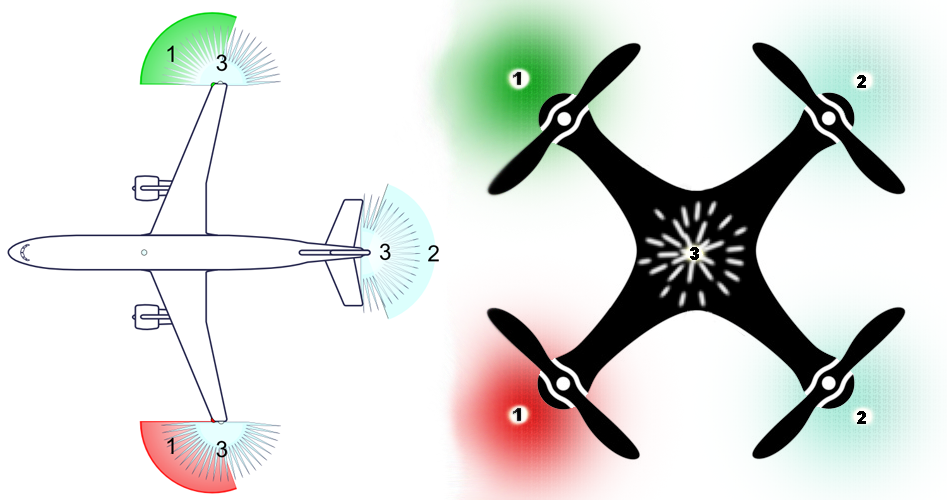
\includegraphics[width=0.90\textwidth]{Figures/esquemalights2.png}
  \caption[Configuration of Position and Anti-Collision for Two Different Aircraft]{Configuration of Position and Anti-Collision for Two Different Aircraft (1-left and right position lights; 2-rear position lights; 3-anti-collision lights}
  \label{fig:esquemalights2}
\end{figure}

The lights range is restricted by the battery power, which usually grants electric power to all the systems inside a sUA. If the selected LEDs consume too much current, the aircraft's maximum time of operation might decrease several minutes. Adding to this, as this thesis is focused in small unmanned aircraft, it is important that the required equipment does not present a high cost to the owner of the equipment, as it would not be cost effective to use a position lights system that costs as much or even more than the rest of the equipment. It may not also present large dimensions and/or weight, so that it does not have a big negative impact in the sUA's overall operation. Finally, the equipment must be accessible, so that any owner can easily buy it: the studied materials should be acquired from stores that are open to the general public and not directly from manufacturers.\\
With this restrictions, it is expected that the required intensities and/or field coverage \citep{Easa2012} will not be met. Because of this, a relation between the characteristics of the aircraft and the required intensities must be developed. \\

As stated in the European Union's Commission Regulation No 859/2008 \citep{EuropeanCommission2008}, the minimum flight visibility limit for aircraft operating in Classes A, B, C, D and E bellow 3050 m and Class G is 5 km. Using this distance as the required range for the proposed position and anti-collision lights system and taking in consideration that sUA travel at a fraction of a normal, utility, aerobatic or commuter aircraft's velocities, provides enough range for manned and unmanned aircraft to see the aircraft and avoid collision.\\
Using equation \ref{eq:intensity} \citep{UnitedStatesCoastGuard2011}, we can calculate the required intensity to achieve the selected range of visibility.\\
\begin{equation}\label{eq:intensity}
I = 3.43 \times 10^{6} \times T \times D^{2} \times K^{-D}
\end{equation}
With:
\begin{itemize}
\item I - luminous intensity in candelas
\item T - threshold factor = $2\times 10^{-7}$ lux
\item D - range of visibility in nautical miles
\item K - atmospheric transmissivity = $0.9$
\end{itemize}
Knowing that 5 km is approximately 2,7 nm, the required intensity is 6.65 cd.\\

Although it may prove difficult to find LEDs with the right field coverage and luminous intensity for the different types of lights (left, right, etc...), it is indispensable that the entire 360\degree are covered and that the limits for each type of light are respected. A possible solution is to use LEDs with a smaller field coverage and to overlap the LEDs of the same type.\\

\section{Material}
\label{section:pmaterial}

To enable the requirements cited in the previous section, the material will be chosen from local electronics stores with websites.\\

\subsection{Selecting LEDs}
The LEDs selected for position lights should have low viewing angles, to enable control of the field of coverage according to CS-23 \citep{Easa2012} and have higher intensities while consuming less power.\\
Due to the bigger field of coverage required for the anti-collision light, the selected LED must have a high viewing angle, while still transmitting with high intensities.\\
The number of LEDs for each position light must be enough to achieve the required field coverage \citep{Easa2012}.\\

The LEDs selected for the left and right position lights are the 5mm Super Bright Red/Green LEDs with part number WW05A3SRP4-N2 and WW05A3SGQ4-N2, respectively, from Wah Wang Holdings. Both have a viewing angle of 25\degree and a forward current of 20 mA. The red LED has a dominant wavelength between 620 and 630 nm, a typical luminous intensity of 8200 mcd and a forward voltage of 2.1 V. The green LED has a dominant wavelength between 515 and 525 nm, a typical luminous intensity equal to 18000 mcd and a forward voltage of 3.1 V. More information can be seen in the respective data sheet \citep{WahWangHoldingsCo.LTD} \citep{WahWangHoldingsCo.LTDb}.\\
The LED selected for the rear position light is the 5mm Super Bright White LED with part number WW05C3SWQ4-N1 from Wah Wang Holdings. With a viewing angle of 20\degree and a forward current of 20 mA, it typically radiates with a luminous intensity equal to 18000 mcd and a forward voltage of 3.1V. More information can be seen in the data sheet \citep{WahWangHoldingsCo.LTDa}.\\
The LED selected for the anti-collision light is the Super Flux Pure White LED with part number OSWA4EZ2C1P-HCRI from OptoSupply. The viewing angle is equal to 120\degree and, with a forward current of 90 mA, it typically radiates with a   luminous intensity of 12000 mcd and a forward voltage equal to 3.1 V. More information can be seen in the data sheet \citep{OptoSupply}.\\
Each LED costs around \euro{0.2}.\\

As the position lights should stay turned on since the start of the operation until the end, there is no need to connect them to the Arduino\texttrademark board. Rather, they should be independent of the designed prototype, connecting directly to the source.\\
The flashing rate of the anti-collision light will be controlled by an Arduino\texttrademark board.\\

\subsection{Selecting Arduino\texttrademark Board}
\label{subsection:arduinoAHP}
Following the Analytic Hierarchy Process (AHP) methodology, one must define several criteria and sub-criteria for the decision making process, based on the main requirements for the Arduino\texttrademark board. Each criteria was then given a relative weight regarding its relevance. All the criteria, including their relative weights, are represented in figure \ref{fig:arduinoahpperc}.\\
\begin{figure}[!htb]
  \centering
  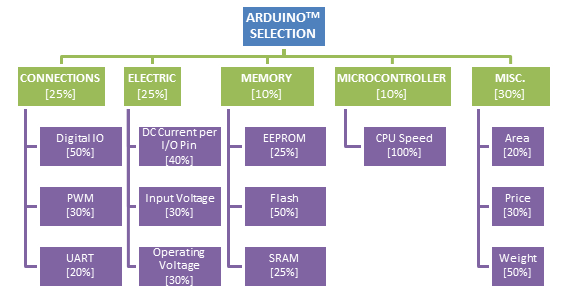
\includegraphics[width=0.90\textwidth]{Figures/arduinoahpperc.png}
  \caption[AHP study hierarchy and criteria relative weights]{AHP study hierarchy and criteria relative weights}
  \label{fig:arduinoahpperc}
\end{figure}
The five main criteria in the design selection process are Connections, Electric, Memory, Microcontroller and Miscellaneous. The Connections criteria accounts for the number of connections of different types (Digital In/Out and Pulse Width Modulation) and the number of Universal Asynchronous Receiver/Transmitter (UART) that enable serial communication. The Electric criteria refers to electric characteristics, such as the DC current available per In/Out pin, the recommended input voltage and the operating voltage. Memory contains three sub-criteria that evaluate the available types of memories (EEPROM, Flash and SRAM). The Microcontroller criterion evaluates the CPU speed. Finally the Miscellaneous criteria accounts for dimensional characteristics of the Arduino\texttrademark board, such as area and weight, as well as its price.\\
The most important sub-criteria is the weight, with a 15\% absolute weight, followed with the number of digital In/Out pins, with 12,5\%, the CPU speed and DC current per In/Out pin, both with 10\%, and finally the price with an absolute weight of 9\%.\\
To enable ranking each Arduino\texttrademark board, each criterion was given an individual scale, ranging from 1 (worst performance) to 3 (best performance), as show in table \ref{tab:ranking} for the 'Connections' and 'Electric' criteria, except for the Operating Voltage (which can only be 3.3 (1 point) or 5 V (3 points) and the recommended Input Voltage which can either be below (1 point) or above (3 points) 11 V.

\begin{table}[!htb]
  \centering
  \caption[AHP sub-criteria ranking for 'Connections' and 'Electric' criteria]{AHP sub-criteria ranking for 'Connections' and 'Electric' criteria}
  \includegraphics[width=0.85\textwidth]{Figures/table1.png}
  \label{tab:ranking}
\end{table}

Each Arduino\texttrademark board was graded on every individual criterion. The final results for the top three boards are shown in table \ref{tab:ahpresults}.

\begin{table}[!htb]
  \centering
  \caption[AHP results for top three boards]{AHP results for top three boards}
  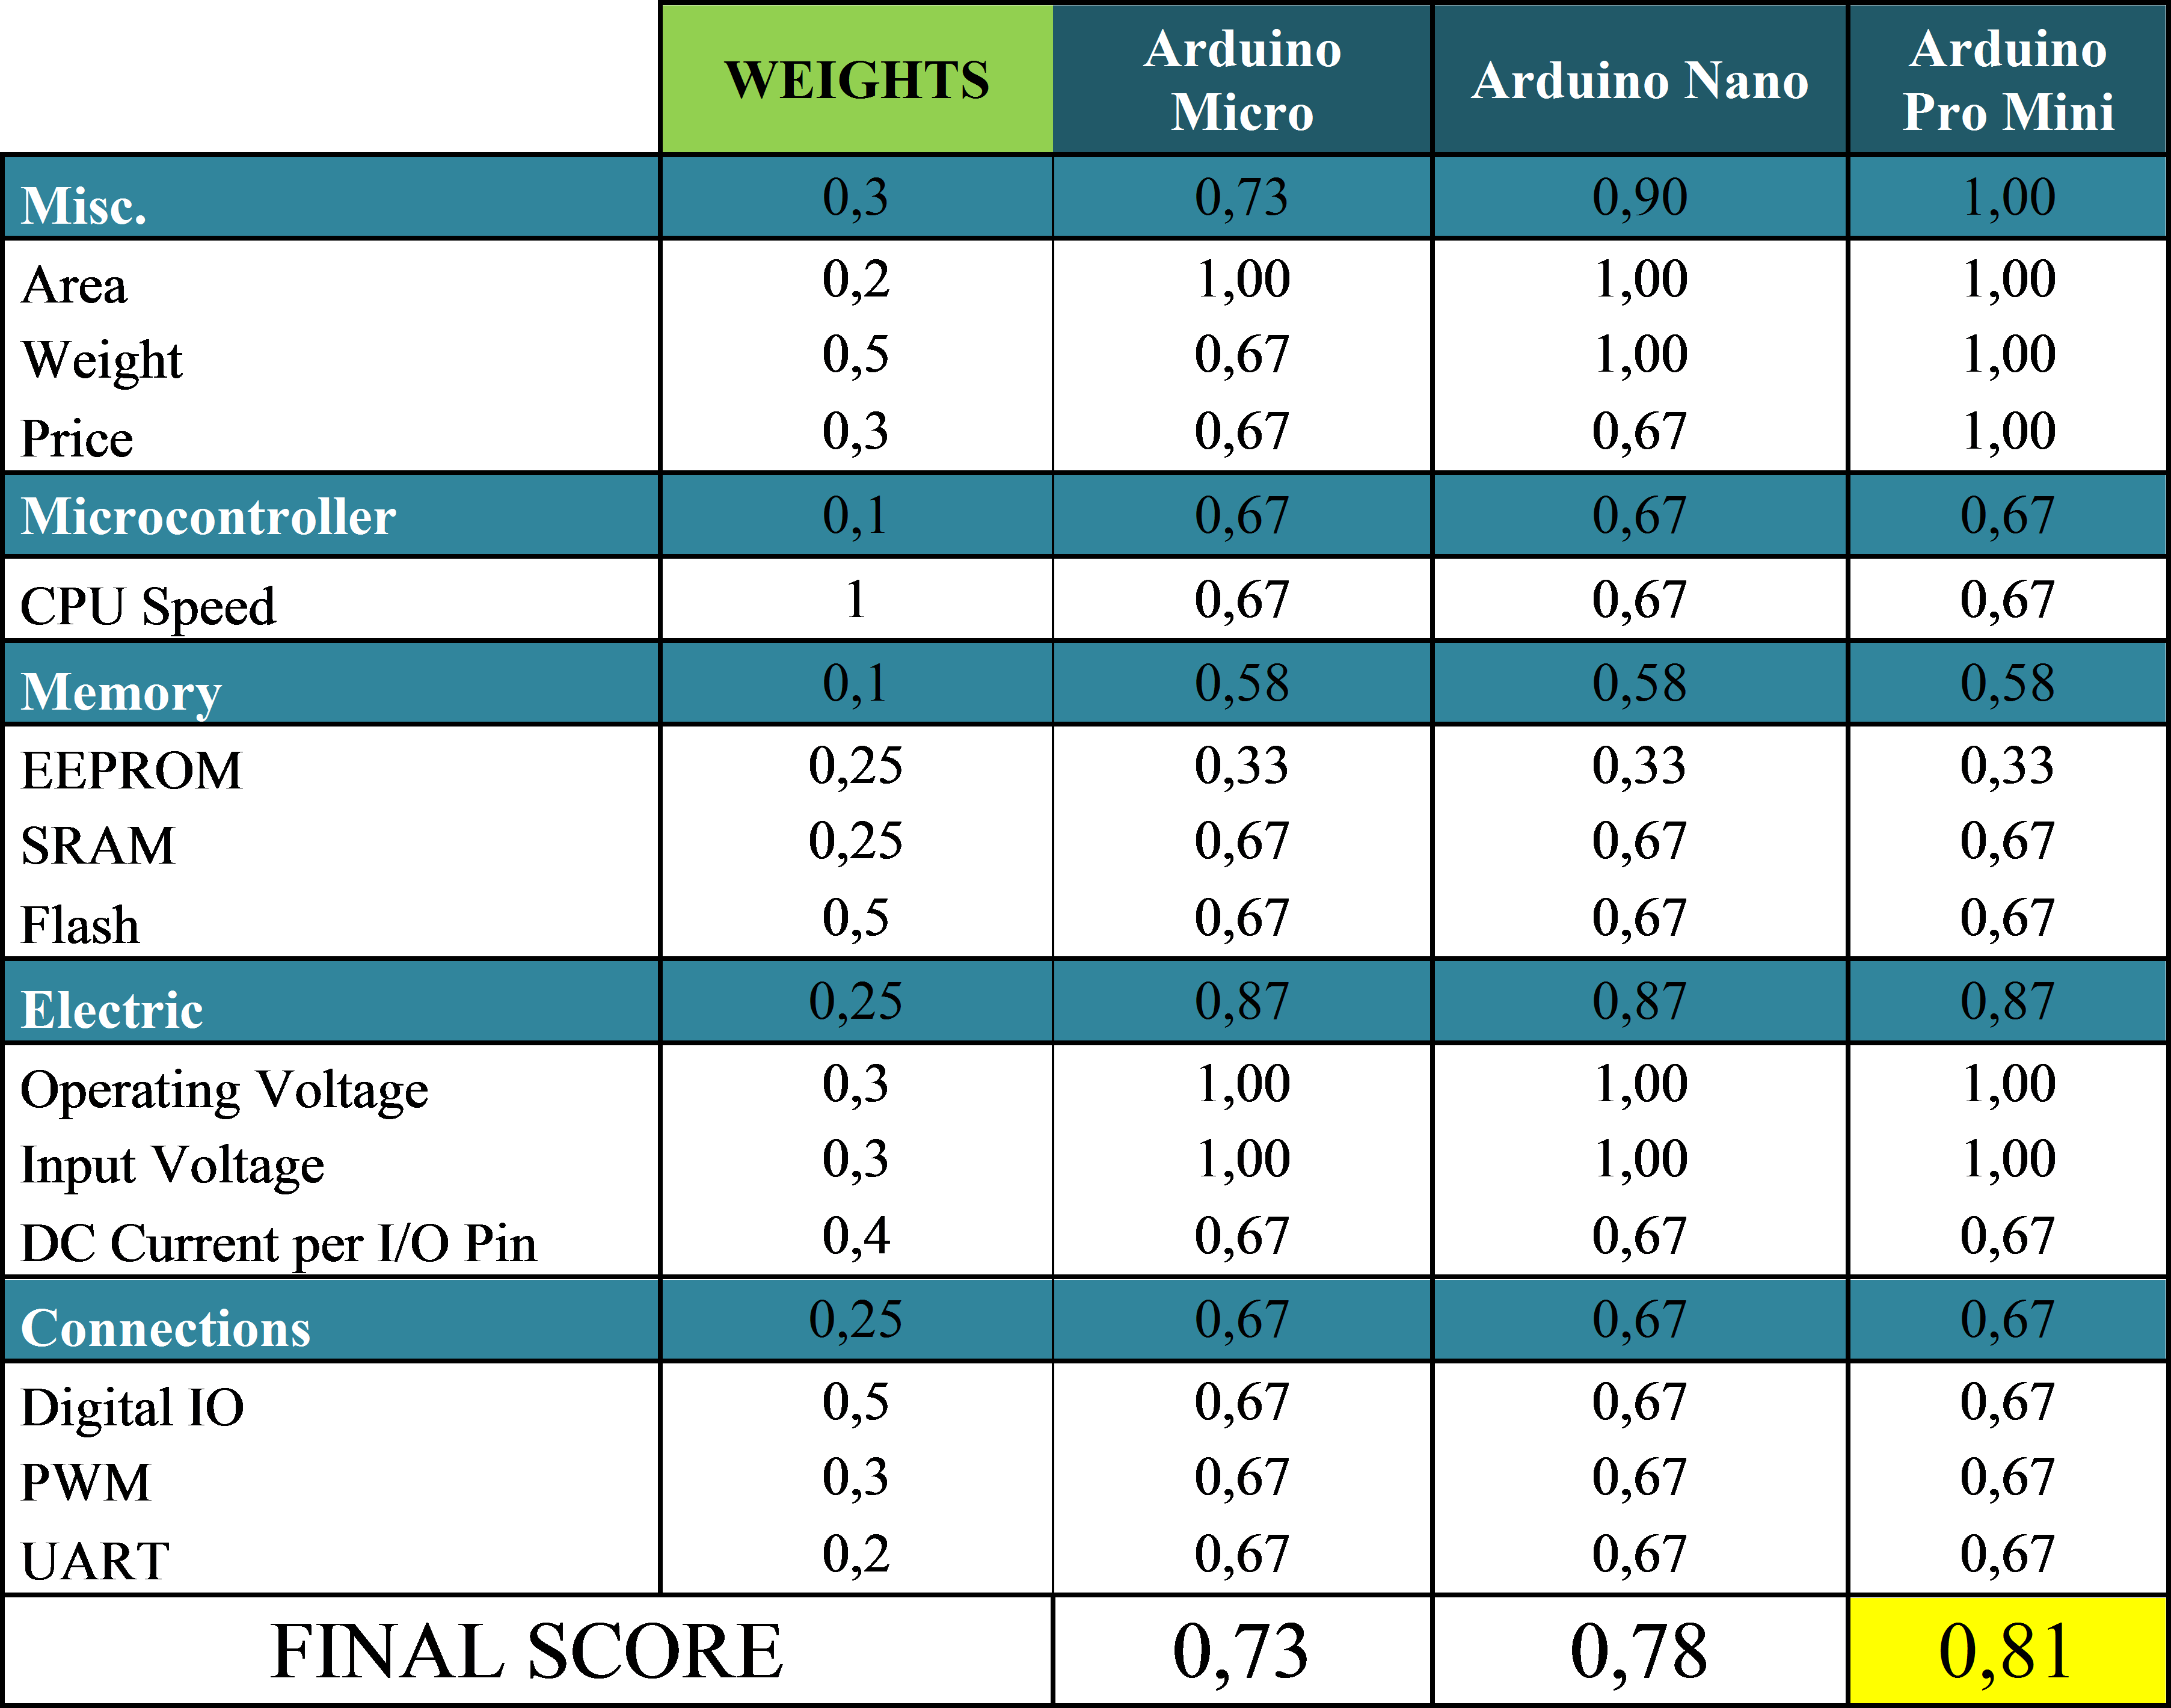
\includegraphics[width=0.75\textwidth]{Figures/ahpresults.png}
  \label{tab:ahpresults}
\end{table}

After analyzing table \ref{tab:ahpresults}, the Arduino\texttrademark board that comes on top is the Arduino\texttrademark Pro Mini which costs \euro{9.80}.\\

Because almost all Arduino\texttrademark boards, including the selected one, have a limit of 40 mA of DC current per output and the LED used for anti-collision light requires 90 mA, not enough current will be given to the LED with a direct connection between an Arduino\texttrademark board and the LED. To provide enough current, while still being able to control the flashing pattern, MOSFETs are needed to switch the LEDs. As the number of LEDs will depend on the aircraft configuration, a MOSFET with a high maximum drain current should be used.\\
The selected MOSFET is the STP55NF06, which has a drain-source-voltage of 60 V and a continuous drain current of up to 50 A. Another important characteristics are the dynamic characteristics, such as the different times. The STP55NF06 has a turn-on delay time of 20 ns, a rise time of 50 ns, a turn-off delay time of 36 ns and a fall time of 15 ns. As the signals that will be used for the anti-collision lights will have duration around several milliseconds, this MOSFET has fast enough dynamic characteristics. This MOSFET has a cost of \euro{1.17}\\
As the maximum drain current is 50 A, and each anti-collision LED is designed for 90 mA, the selected MOSFET can easily control more than 10 LEDs, which is expected to be enough for most aircraft types.\\

\subsection{Selecting resistors}
\label{subsection:resistors}
In order to obtain the desired field coverage, the number of LEDs required of each type can be seen in table \ref{tab:voltagecurrent}. To achieve the desired DC current, different configurations were adopted for each type of LED, as can be seen in figures~\ref{fig:diagrams:1}--\subref{fig:diagrams:4}: the Left Position Light will have all five LEDs in series (figure~\ref{fig:diagrams:1}), the Right Position Light will have the LEDs in one series of two and one series of three (figure~\ref{fig:diagrams:2}), the Rear Position Light will have two series of three LEDs and two series of one LED (figure~\ref{fig:diagrams:3}), and finally the Anti-Collision Light will have all three LEDs connected in series (figure~\ref{fig:diagrams:4}).\\

\begin{figure}[ht]
  \centering
  \subfigure[][]{
    \label{fig:diagrams:1} 
    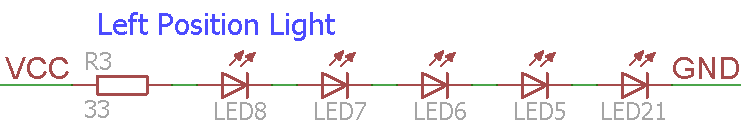
\includegraphics[]{Figures/EsquemasLights/leftpositionlight.png}
  }
  \hspace{8pt}
  \subfigure[][]{
    \label{fig:diagrams:2} 
    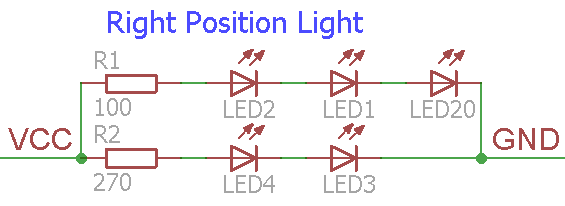
\includegraphics[]{Figures/EsquemasLights/rightpositionlight.png} 
  }\\
  \subfigure[][]{
    \label{fig:diagrams:3} 
    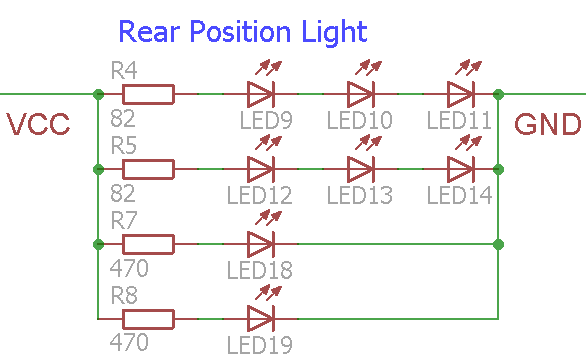
\includegraphics[]{Figures/EsquemasLights/rearpositionlight.png}
  }
  \hspace{8pt}
  \subfigure[][]{
    \label{fig:diagrams:4} 
    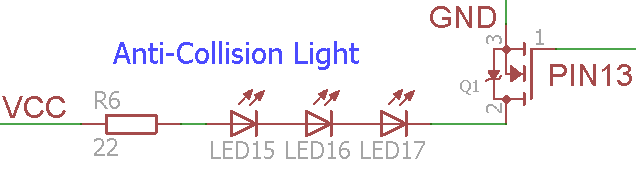
\includegraphics[]{Figures/EsquemasLights/anticollisionlight.png} 
  }
  \caption[Schematic Diagram of each Light]{Schematic Diagram of each Light:
			\subref{fig:diagrams:1} describes the Left Position Light;
			\subref{fig:diagrams:2} describes the Right Position Light;
			\subref{fig:diagrams:3} describes the Rear Position Light; and,
			\subref{fig:diagrams:4} describes the Anti-Collision Light.}%
  \label{fig:diagrams}%
\end{figure}

The required resistances are then calculated in order to obtain the correct current in each LED, using easily available resistance values. As the aircraft used for testing uses a 3S battery (11.1V), to correctly dimension the connections, we have the forward voltage and continuous forward current for each LED and the number of LEDs of each type in table \ref{tab:voltagecurrent}.\\
\begin{table}[!htb]
\centering
\caption[Forward Voltage, Continuous Forward Current and Number of LEDs for each Position and Anti-Collision Light \citep{OptoSupply}\citep{WahWangHoldingsCo.LTD}\citep{WahWangHoldingsCo.LTDa}\citep{WahWangHoldingsCo.LTDb}]{Forward Voltage, Continuous Forward Current and Number of LEDs for each Position and Anti-Collision Light \citep{OptoSupply}\citep{WahWangHoldingsCo.LTD}\citep{WahWangHoldingsCo.LTDa}\citep{WahWangHoldingsCo.LTDb}}
\label{tab:voltagecurrent}
\begin{tabular}{@{}llll@{}}
\toprule
LED                    & Forward Voltage (V) & Continuous Forward Current (mA) & Number of LEDs \\ \midrule
Green                  & 3.1                 & 20		&	5                       \\
Red                    & 2.1                 & 20       &	5                       \\
White (Rear)           & 3.1                 & 20       &	8                       \\
White (Anti-Collision) & 3.1                 & 90       &	3                       \\ \bottomrule
\end{tabular}
\end{table}
The voltage drop across each resistor can then be calculated according to equation \eqref{eq:voltagedrop}, where each LED's forward voltage depends on the number of LEDs.
\begin{equation}\label{eq:voltagedrop}
V_{D}=V_{S}-V_{F}
\end{equation}
With:
\begin{itemize}
\item $V_{D}$ - Resistor's voltage drop
\item $V_{S}$ - source's voltage
\item $V_{F}$ - total LED's forward voltage 
\end{itemize}
According to figures~\ref{fig:diagrams:1}--\subref{fig:diagrams:4}, the total LED's forward voltage for each type is equal to:
\begin{itemize}
\item Green (series of 3)- $V_{F} = 9.3 V$
\item Green (series of 2)- $V_{F} = 6.2 V$
\item Red - $V_{F} = 10.5 V$
\item White (Rear series of 3) - $V_{F} = 9.3 V$
\item White (Rear series of 1) - $V_{F} = 3.1 V$
\item White (Anti-Collision) - $V_{F} = 9.3 V$
\end{itemize}
The obtained values for each resistor's voltage drop are shown in table \ref{tab:voltageresistance}. It is then possible to calculate the required resistance with Ohm's law, shown in equation \eqref{eq:ohm}.
\begin{equation}\label{eq:ohm}
R=\dfrac{V}{I}
\end{equation}
The results are shown in table \ref{tab:voltageresistance}.
\begin{table}[!htb]
\centering
\caption[Voltage Drop and Resistance Required for each Position Light LED's Resistor]{Voltage Drop and Resistance Required for each Position Light LED's Resistor}
\label{tab:voltageresistance}
\begin{tabular}{@{}lll@{}}
\toprule
LED                    		& Resistor's voltage drop (V) 	& Resistance ($\Omega$) \\ \midrule
Green (series of 3)    		& 1.8							& 90                   \\
Green (series of 2)    		& 4.9							& 245                   \\
Red                    		& 0.6							& 30                   \\
White (Rear series of 3)    & 1.8							& 90                    \\
White (Rear series of 1)    & 8.0							& 400                   \\
White (Anti-Collision) 		& 1.8							& 20                    \\ \bottomrule
\end{tabular}
\end{table}

The obtained values for the resistance were then changed for the nearest higher rated resistor, in order to use more available material while still protecting the LEDs:
\begin{itemize}
\item Green (series of 3)- R = 100$\Omega$
\item Green (series of 2)- R = 270$\Omega$
\item Red - R = 33$\Omega$
\item White (Rear series of 3) - R = 100$\Omega$
\item White (Rear series of 1) - R = 470$\Omega$
\item White (Anti-Collision) - R = 22$\Omega$
\end{itemize}
Each resistor as an approximate cost of \euro{0.1}.\\

\section{Material Testing}
\label{section:pmaterialtesting}
One of the most important characteristic of a Position Lights System is its range.\\
To test the equipment's range, a test procedure was created (Test Procedure Lights), as can be seen in section \ref{visualmaterial}, which consisted in obtaining an evaluation of visibility of the LEDs by several users. \\
To allow all LEDs to be tested at the same time, a schematic was designed, as seen in figure \ref{fig:testesquemaleds}, that allows an Arduino\texttrademark board to control all LEDs, following the diagram in figure \ref{fig:lightstestdiagram}. The code turns each position LED on for two seconds and, in the end of each cycle, the Anti-Collision Light transmits the letter 'D' two times in Morse Code. \\
\begin{figure}[!htb]
  \centering
  \includegraphics[width=0.90\textwidth]{Figures/testeesquemaleds.png}
  \caption[Schematic for Position Lights and Anti-Collision Systems Test]{Schematic for Position Lights and Anti-Collision Systems Test}
  \label{fig:testesquemaleds}
\end{figure}

\begin{figure}[!htb]
  \centering
  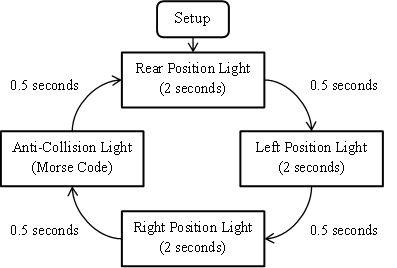
\includegraphics{Figures/LightsTestDiagram.png}
  \caption[Arduino\texttrademark Script Diagram]{Arduino\texttrademark Script Diagram}
  \label{fig:lightstestdiagram}
\end{figure}
The script 'DroneTest.ino' allows the subjects of the test to evaluate all lights on a straight line at several ranges between 50 and 350m, as shown in figure \ref{fig:ranges2}. To acquire the range during the test, an Android application was used, 'GPS Distance Location Tracker', which uses the GPS signal to track movement, including distances.\\
\begin{figure}[!htb]
  \centering
  \includegraphics[width=0.90\textwidth]{Figures/ranges2.png}
  \caption[Distances for Position and Anti-Collision lights range test]{Distances for Position and Anti-Collision lights range test}
  \label{fig:ranges2}
\end{figure}

In order to avoid fluctuations on the LEDs' intensity, a continuous power provider was used.\\
The test then consisted in each individual walking on a straight line, half towards and the other half away from the system to allow the subject to evaluate all LED separately, providing a qualitative evaluation (grade between 1 and 10). The test subjects gave an assessment of the lights intensity at the 50, 100, 150, 200, 250, 300 and 350m mark.\\

\section{Prototyping}
\label{section:pprototypes}

To provide an implementation example, the system will be adapted to a quadcopter.\\
Using the quadcopter's standard front side, the left and right position lights will be composed by 5 LEDs each to achieve a field coverage of 110\degree \citep{Easa2012}, where each LED overlaps the next one by 6\degree ; the rear position light will be composed by 8 LEDs to achieve a field coverage of 140\degree \citep{Easa2012}, where each LED overlaps the next one 3.4\degree . By overlapping LEDs, it is easier to ensure a complete field coverage, avoiding gaps caused by higher manufacture margins or defect's probability from the cheaper LEDs. Finally the anti-collision light will be composed by 3 LEDs, to concentrate the highest intensities of the LED around the aircraft and not on top of it. This configuration is shown in figure \ref{fig:esquemalights3}.\\

\begin{figure}[!htb]
  \centering
  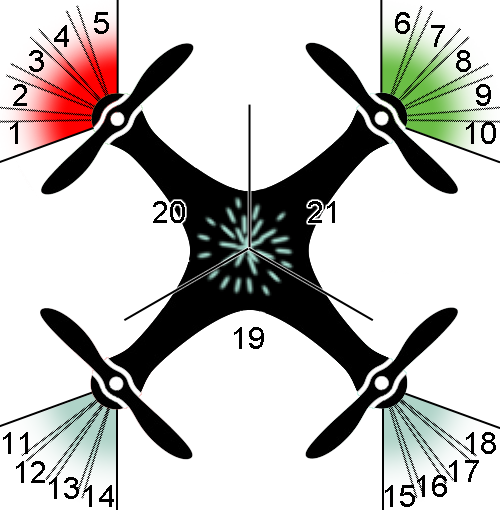
\includegraphics[width=0.6\textwidth]{Figures/esquemalights3.png}
  \caption[Configuration of Position and Anti-Collision on Quadcopter]{Configuration of Position and Anti-Collision on Quadcopter (1,2,3,4,5 - Left Position Light; 6,7,8,9,10 - Right Position Light; 11,12,13,14,15,16,17,18 - Rear Position Light; 19,20,21 - Anti-Collision Light}
  \label{fig:esquemalights3}
\end{figure}

To distribute power to all LEDs, a PCB was designed. As can be seen in figure \ref{fig:schematicluzes}, this board connects to the aircraft's power distribution board and to pin 13 of the Arduino\texttrademark Pro Mini.

\begin{figure}[!htb]
  \centering
  \includegraphics[width=0.80\textwidth]{Figures/schematicluzes.png}
  \caption[Schematic for Position and Anti-Collision Light System]{Schematic for Position and Anti-Collision Light System}
  \label{fig:schematicluzes}
\end{figure}

\subsection{Controlling the Anti-Collision LED}
\label{subsection:pcontrolblink}

To control the blinking pattern of the Anti-Collision LED, a simple C library was developed.\\
The script 'morseaircraft.h', contains all variables and functions available.\\
On 'morseaircraft.cpp', the function 'MorseAircraft', of the class with the same name, is given the type of aircraft, using the nomenclature explained in subsection \ref{subsection:aircraftypes} (for example 'H' for helicopters), when called. The function then provides the message that will be transmitted with the Anti-Collision Lights, the correct period for the Morse code, the number of bits transmitted (called order) and the type of aircraft coded in decimal base:
\begin{enumerate}
\setcounter{enumi}{-1}
\item A - Unpowered air sports
\item B - Hot air balloons
\item C - Cargo aircraft
\item[] ...
\setcounter{enumi}{11}
\item S - Powered air sports
\item T - Pressurized passenger aircraft required to carry ACAS
\item UA - Unmanned unpowered air sports
\item UB - Unmanned hot air balloons
\item[] ...
\setcounter{enumi}{26}
\item UT - Unmanned pressurized passenger aircraft required to carry ACAS
\end{enumerate}

The other function provided in 'morseaircraft.cpp' is flash() which controls the on and off times of the Anti-Collision Lights, correctly transmitting the Morse code. It will also rotate the message so that the least precedent bit always contains the bit that will be transmitted next.

\subsection{ISR's Quadcopter}
\label{subsection:pisr}

The visual spectrum solution was introduced on a quadcopter as implementation example, using the configuration shown in figure \ref{fig:esquemalights3} and the equipment from section \ref{section:pmaterial}.\\
The position lights were fixed to the bottom of the engines, to avoid interference with their operation. The anti-collision light was mounted on top of the IR sense and avoid prototype develop in chapter \ref{chapter:active}.\\
The equipped aircraft can be seen in figures~\ref{fig:visualprototype1}--\subref{fig:visualprototype2}, from its right side.\\
\begin{figure}[ht]
  \centering
  \subfigure[][]{
    \label{fig:visualprototype1} 
    \includegraphics[width=0.45\textwidth]{Figures/visualprototype1.png}
  }
  \hspace{8pt}
  \subfigure[][]{
    \label{fig:visualprototype2} 
    \includegraphics[width=0.45\textwidth]{Figures/visualprototype2.png} 
  }\\
  \caption[Aircraft with Visual Spectrum Solution Implemented]{Aircraft with visual spectrum solution implemented:
			\subref{fig:visualprototype1} with anti-collision light off; and,
			\subref{fig:visualprototype2} with anti-collision light on.}%
  \label{fig:visualprototype}%
\end{figure}

The total cost of the acquired material is \euro{20} with an included \euro{4} for miscellaneous material such as wire and solder.\\

After assembling the prototype on the quadcopter, the aircraft was flown in order to check the prototype behavior during flight, as shown in figures \ref{fig:visualground}--subref{fig:visualflight}.\\
\begin{figure}[ht]
  \centering
  \subfigure[][]{
    \label{fig:visualground} 
    \includegraphics[width=0.45\textwidth]{Figures/visualground.png}
  }
  \hspace{8pt}
  \subfigure[][]{
    \label{fig:visualflight} 
    \includegraphics[width=0.45\textwidth]{Figures/visualflying.png} 
  }\\
  \caption[Aircraft with Visual Spectrum Solution Implemented during Flight]{Aircraft with visual spectrum solution implemented during flight:
			\subref{fig:visualprototype1} ready for take-off; and,
			\subref{fig:visualprototype2} mid flight.}%
  \label{fig:visual}%
\end{figure} % file "Thesis_PassiveSolution.tex"

%%%%%%%%%%%%%%%%%%%%%%%%%%%%%%%%%%%%%%%%%%%%%%%%%%%%%%%%%%%%%%%%%%%%%%%%
%                                                                      %
%     File: Thesis_ActiveSolution.tex                                  %
%     Tex Master: Thesis.tex                                           %
%                                                                      %
%     Author: Miguel Fonseca                                           %
%     Last modified : 8 Jul 2015                                       %
%                                                                      %
%%%%%%%%%%%%%%%%%%%%%%%%%%%%%%%%%%%%%%%%%%%%%%%%%%%%%%%%%%%%%%%%%%%%%%%%

\chapter{Infrared Solution}
\label{chapter:active}
As there is still no global procedure to register UA, the use of unique identification for a sense and avoid system should be averted. It is important to notice that, in order to prevent collisions, the specific knowledge of the intruder's identification is not required. Only the type of aircraft is required so that right-of-way rules may be applied.\\
The proposed sense and avoid system should not be expensive to allow easy access for the owners of cheap small unmanned aircraft. It is also important to use small and lightweight equipment/materials that is readily available from local electronics stores or websites, so that its implementation has a good cost/benefit relation.\\
Finally, the system should provide detection as well as relative position between multiple unmanned aircraft, to enable collision avoidance by corrections of the original flight path.\\

\section{Choosing the solution}
\label{section:choosing}
\subsection{Electromagnetic spectrum's frequency}
\label{subsection:eospectrum}
In order to use a wireless cooperative system, an operating frequency from the electromagnetic spectrum, depicted in figure \ref{fig:spectrum}, has to be chosen.
\begin{figure}[!htb]
  \centering
  \includegraphics[width=0.8\textwidth]{Figures/spectrum.png}
  \caption[Electromagnetic Spectrum \citep{Haynes}]{Electromagnetic Spectrum \citep{Haynes}}
  \label{fig:spectrum}
\end{figure}
\subsubsection{Radio and Micro waves}
The radio and microwaves' spectrum are highly regulated and usually require a permit for operation. This area of the electromagnetic spectrum is already highly used in many different technologies in aviation, such as ADS-B and TCAS, or for common use, like radio and television, among others. This type of technology generally requires high power equipment to transmit the signal, which sUA cannot provide due to their low power batteries.\\
To avoid using high power equipment in the aircraft, it is possible to use a network of communication already in use, such as the GSM network. This type of network allows the user to operate with small, low power equipment, using instead several fixed antennas with high gain to provide the required coverage. This solution has several problems however. Because the aircraft would depend on fixed equipment and omni-directional antennas for communication, it is harder to compute the aircraft's localization: one way to do this is triangulation, which requires the aircraft to be in range of several antennas; and another way is for the aircraft to use another source of localization, such as GNSS, which has been hacked in the past \citep{Emspak2011} \citep{BBCNewsTechnology2012} and may provide errors in GPS denied areas. Adding to this, each aircraft would be required to have a unique identification and, as there is still no international standard, it is impossible to ask for it at this time. Using the same network as cellphone users would have other problems: for example, during certain events, the GSM network is not able to withstand the number of users, which would deprive an aircraft of its main sense and avoid system.\\
\subsubsection{Visible, Ultraviolet and higher frequency waves}
Ultraviolet (UV) waves interact with the Earth's atmosphere by scattering. Although this facilitates their propagation under non-line-of-sight communications, it would not be ideal to provide relative position \citep{Cruz}.\\
Frequencies above the UV spectrum, such as x-rays and gamma rays, may have several risks for human health due to their high levels of energy \citep{Waltz2008}. \\
Visual light spectrum has too much ambient noise, as can be seen in figure \ref{fig:solarspectrum}, which requires high processing capabilities to enable detection.\\
\subsubsection{Infrared spectrum}
The remaining Infrared waves may have wavelengths between 750 nm to 1 mm (or frequencies from 400 THz to 300 GHz). The International Commission on Illumination (CIE) divides the infrared radiation in three different sections: IR-A (0.78 $\mu$m to 1.4 $\mu$m), IR-B (1.4 $\mu$m to 3 $\mu$m) and IR-C (3 $\mu$m to 1000 $\mu$m) \citep{Taylor2000}. \\
Although there are some reported cases of humans being able to see the lower wavelength infrared \citep{Cox}, the majority is not able to see above wavelengths of 780 nm , which means that using an infrared wave for communication purposes does not create visual pollution.\\
Adding to this, the infrared spectrum is unregulated \citep{Hou2015}, except for health concerns \citep{Ghassemlooy2006}, and it is not necessary a license to operate in these frequencies \citep{Hou2015}. Although there is still some infrared radiation from the sun that reaches the sea level, a large percentage is filtered by the atmosphere, particularly in some wavelengths due to the interaction with molecules such as O$_{2}$ and H$_{2}$O, as can be seen in figure \ref{fig:solarspectrum}.\\
\begin{figure}[!htb]
  \centering
  \includegraphics[width=0.70\textwidth]{Figures/SolarSpectrum.png}
  \caption[Solar Radiation Spectrum \citep{Rohde2007}]{Solar Radiation Spectrum \citep{Rohde2007}}
  \label{fig:solarspectrum}
\end{figure}

Another important advantage is that, by using a completely different wavelength than other communication systems used in aviation, such as TCAS and ADS-B, the proposed system is transparent to them. This means that an infrared communication system cannot interfere with the systems in operation nowadays, with the downside of not being able to receive and cooperate with them.\\
Because the infrared waves have a behavior much different from radio and microwaves, it does not generate radio-frequency interference (RFI), which is known for creating disturbances in electrical circuits due to electromagnetic radiation or electromagnetic induction \citep{Hou2015}. This is essential in a system that operates in close proximity to the autopilot or flight management system of an aircraft through cable communications.\\

Despite this, there are several problems with IR-B and IR-C frequencies. There is too much noise generated by objects and animals on the Earth's surface to use IR-C. Adding to this, the atmosphere has poor transmission on wavelengths between 5 to 8 $\mu$m \citep{Cox}. Finally, the typical used silicon photodiodes are not sensitive above 1100 nm \citep{Ryer.1998} which turns the IR-B frequencies expensive to work with.\\

The IR-A wavelengths also have some disadvantages. The main disadvantage is its range: IR signals may be adversely affected by dust, scintillation, smoke and some weather conditions \citep{Pauluzzi1992}. Weather conditions, such as fog, rain and snow, can generate different amounts of attenuation: depending on its density, fog can decrease the range of communication from 30 m in a clear day down to 7.5 m, with a total attenuation of 12 dB \citep{Pauluzzi1992}. For comparison, heavy rain would only decrease the same signal to 28 m, with an even smaller decrease generated by dust and snow \citep{Pauluzzi1992}. Scintillation, which is a fluctuation in the refraction index of the air due to uneven heating of air, may cause a reduction in range to half the original value \citep{Pauluzzi1992}.\\ 
The fact that IR waves cannot penetrate walls has the disadvantage of creating zones where the signal doesn't reach. Because of this, a sense and avoid system that uses the infrared spectrum may present poor results in places with big obstacles, such as cities and mountains, or indoors: if an intruder is located behind an obstacle, it will not be detected until both aircraft are too close. Adding to this, because infrared waves reflect in several surfaces, there is also the danger of multipaths and the risk of aircraft receiving its own signal. Multipaths may generate inter-symbol interference \citep{Ghassemlooy2006} or, in the specific case in study, the illusion of an aircraft in a position that is not correct, while an aircraft receiving its own signal will detect an aircraft that does not exist.\\ 
As UV waves, the infrared spectrum can also pose a risk to human health, specially to the eyes. This risk is minimized when using LEDs as the source of infrared waves, instead of lasers which have a much more concentrated beam \citep{Ghassemlooy2006}. There is also risk to the skin but this requires power levels much higher than for the eyes. Finally, long-term exposure to IR waves is negligible, as the ambient light sources are constantly submitting our bodies to much higher radiation levels than the studied systems \citep{Kahn1997}. Even so, the risk for human health must be accounted for when selecting the material for the prototype.\\

In the IR-A, or near infrared, there could be several wavelength options. O$_{2}$ has a significant impact in filtering the Sun's radiation with 0.76 $\mu$m of wavelength without reducing its transmission too much. H$_{2}$O has a similar effect for radiation with wavelength around 0.72 $\mu$m, 0.82 $\mu$m, 0.94 $\mu$m and 1.1 $\mu$m \citep{Cox} \citep{Cornelius}.\\
The available wide bandwith at this range (200 THz in the 700-1500 nm range) \citep{Ghassemlooy2006} cannot penetrate walls, which decreases significantly the probability of interfering with other applications that use infrared waves \citep{Pauluzzi1992}, such as remote controls.\\
The 940/950 nm wavelength is broadly used in remote controls which means that emitters and receivers have a very low cost market \citep{Hou2015} \citep{Rao2013}, which is highly desirable.\\

There are two main sources used to transmit infrared radiation in the 940/950 nm wavelength: Lasers and LEDs. Although lasers have broader bandwidth, the acquisition costs are higher \citep{Pauluzzi1992} and they have several restrains due to eye safety issues \citep{Ghassemlooy2006}, as previously discussed. LEDs have relaxed eye safety due to the dispersion of power through the wider angular beam. Adding to this, the laser's smaller angular beam would not be appropriate to provide the required angular coverage.
\subsection{Communication Type}
\label{subsection:communication}
As in chapter \ref{chapter:passive}, the proposed system uses an approach similar to a solution already used in aviation. \\
The Very High Frequency Omni-directional Range (VOR) is a conventional radio navigation aid which encodes the azimuth as the relation between two modulations: reference and variable phase modulations \citep{InternationalCivilAviationOrganization2006}. The difference between the two signals' phases is equal to the angle between the magnetic north and the receiver. This enables the pilot of an aircraft to know his position relative to the VOR.\\
The proposed system replaces the radio signals with IR transmitting LEDs and the phase difference with a communication protocol. To avoid moving parts, several transmitting sectors will be designed, each with one LED, as well as different reception sectors, each with one receiver. The number of LEDs and receivers must be enough to cover all horizontal 360\degree, without overlapping, either for transmission and reception. The relative position will be given by the number of the receiver and by the information sent by each LED. This way, the aircraft can compute the intruders direction and predict a possible collision.\\
Adding to this, the transmitted message will contain the transmitting aircraft's type, so that right-of-way rules can be applied.\\

Consumer IR is the utilization of infrared for communication between consumer electronics. The near-infrared band, or IR-A, is always used so that cheap PIN diodes can be used as receivers. IR receivers used in consumer electronics usually have a preamplifier and a package which behaves as an IR filter \citep{Vishay2013}. To distinguish the signal from the ambient noise, the signal is modulated at a predetermined frequency, usually between 30 and 60 kHz, by turning the carrier on and off (Pulse Width Modulation or PWM). Also because of ambient generated noise, the receivers are adapted for short bursts of communication which contain information encoded into bits \citep{Vishay2013}. 
Although there are many different consumer IR protocols, the most used are Philips' RC-5 and RC-6, the Japanese NEC and the SONY's SIRC. The adopted one was the RC-5, due to the available knowledge about the correct timings and structure of the code, as listed in figure \ref{fig:rc5protocol}.\\
\begin{figure}[!htb]
  \centering
  \includegraphics[width=0.9\textwidth]{Figures/rc5protocol.jpg}
  \caption[RC5-5 Philips Protocol details \citep{Infrarossidotit2009}]{RC5-5 Philips Protocol details \citep{Infrarossidotit2009}}
  \label{fig:rc5protocol}
\end{figure}

As can be seen in figure \ref{fig:rc5protocol}, the RC-5 protocol uses bi-phase modulation (or Manchester code), where each data bit is coded into a sequence of lows and highs with the same duration: a '0' is represented by a high followed by a low, while a '1' is the inverse. The Manchester coding has several benefits, among which \citep{Pauluzzi1992}:
\begin{itemize}
\item "The power spectral density of the signal is shifted away from DC which helps to reduce low frequency (power line) interference, and it also eliminates baseband wander at the receiver."
\item "clock recovery is made simple since there is a logic transition in the center of every bit interval"
\item duty cycle of 50\% for bits 0 and 1
\end{itemize}
To avoid interference with consumer electronics, such as televisions, instead of using the standard 36 kHz modulation, a higher frequency of 56 kHz will be used. As can be seen in figure \ref{fig:receiverfrequency}, the responsivity of a 36 kHz receiver for a 56 kHz modulated signal is under 0.2.\\
\begin{figure}[!htb]
  \centering
  \includegraphics[width=0.7\textwidth]{Figures/receiverfrequency.png}
  \caption[IR Receiver TSOP48's Frequency Dependence of Responsivity \citep{Vishay2015}]{IR Receiver TSOP48's Frequency Dependence of Responsivity \citep{Vishay2015}}
  \label{fig:receiverfrequency}
\end{figure}

As the RC-5 has a PWM modulation as well as the Manchester coding, the duty cycle decreases to 25\% , which is desired to reduced the battery's toll.\\

The original RC-5 signal, as can be seen in figure \ref{fig:rc5protocol}, is composed by:
\begin{itemize}
\item 2 start bits
\item 1 toggle bit
\item 5 bits to represent the IR device address
\item 6 bits with the command
\end{itemize} 


\subsection{Proposed Solution}
\label{subsection:solution}
The proposed solution, as seen in figure \ref{fig:irdiagram}, uses 16 transmitting sectors, each with one IR LED with an angle of half transmission equal to 20\degree , located all around the prototype and 4 receiving sectors, each with one IR receiver with an angle of half transmission equal to 90\degree , located at the center so that no overlapping can happen in the reception.\\
\begin{figure}[!htb]
  \centering
  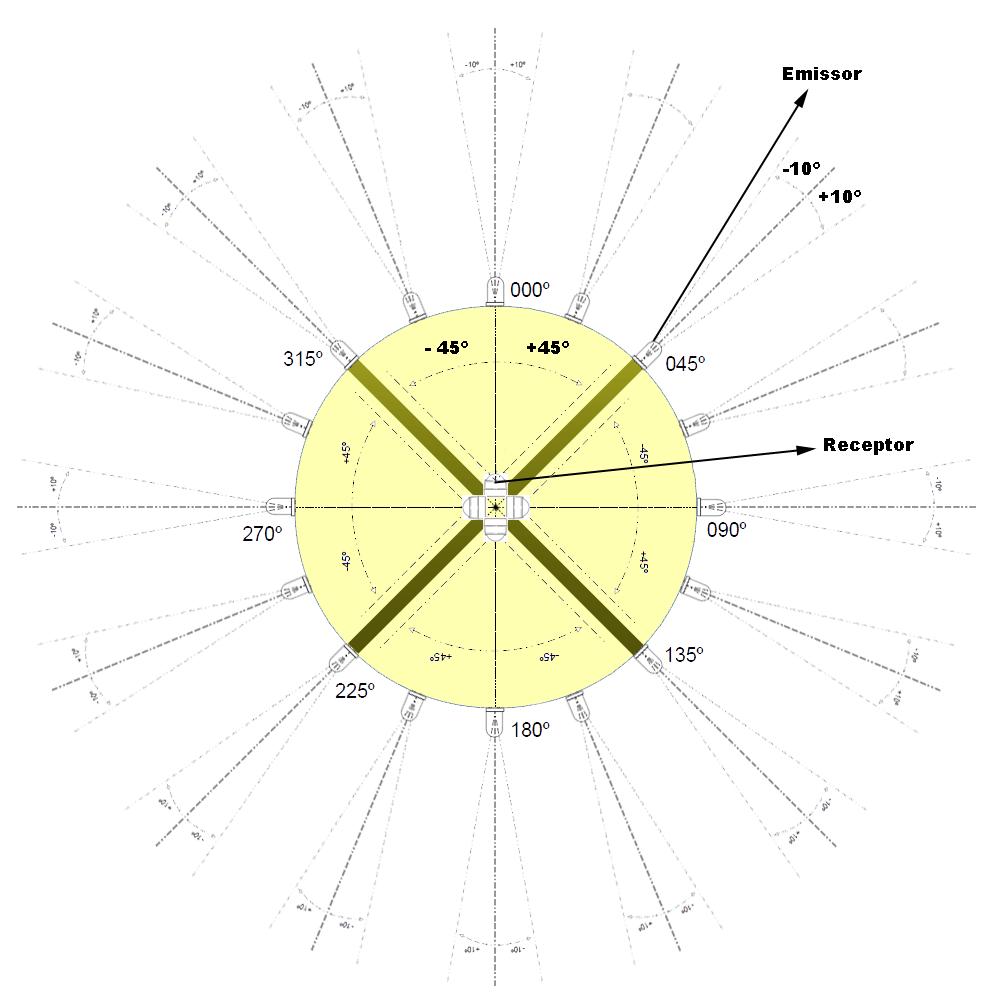
\includegraphics[width=0.8\textwidth]{Figures/esquemaIR16.png}
  \caption[IR diagram]{IR diagram}
  \label{fig:irdiagram}
\end{figure}

Because the PWM modulation frequency has been changed, the address bits are no longer necessary and so the available 5 bits will be used to transmit the aircraft's category. Adding to this, as the prototype only requires 16 transmitting sectors, we only need 4 bits to send their identification. And so, the transmitted message will be composed by:
\begin{itemize}
\item 2 start bits
\item 1 toggle bit
\item 5 bits to represent the type of aircraft
\item 4 bits with sector identification
\end{itemize} 
With this, the transmitted signal is shorter than the standard RC-5, which will enable an increase in the transmission rate.\\

The prototype will only handle the sensing of intruders, as the tracking and collision avoidance may require more processing power than an Arduino\texttrademark board can offer. After receiving a signal, the Arduino\texttrademark board should send it to the autopilot, which is then responsible to determine if any measures are necessary to avoid collision and which maneuvers should be applied.\\

\section{Material}
\label{section:material}
To enable the requirements cited in the previous section, the material will be chosen from websites from local electronics stores. The required materials are shown in figure \ref{fig:irblockdiagram}.\\
\begin{figure}[!htb]
  \centering
  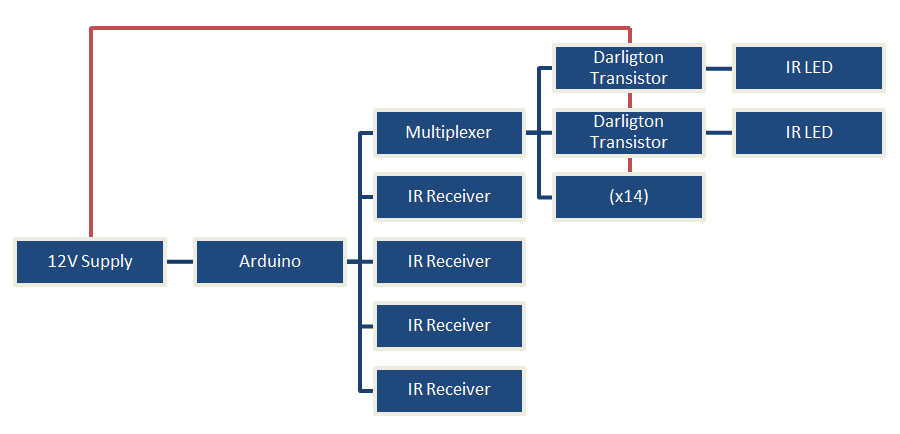
\includegraphics[width=0.8\textwidth]{Figures/blocoscompleto.png}
  \caption[Block Diagram of the IR Anti-Collision System]{Block Diagram of the IR Anti-Collision System}
  \label{fig:irblockdiagram}
\end{figure}

The Arduino\texttrademark board was chosen according to the AHP already explained in section \ref{subsection:arduinoAHP}. The Arduino\texttrademark Pro Mini is responsible for controlling the transmission by the LEDs as well as the reception by the receivers.\\
Most Arduino\texttrademark boards can only perform one task at a time. Because of this, the prototype will only be able to transmit or receive at any given time, and the transmission can only happen in one LED at a time, as each LED will transmit a different message which identifies its sector.\\
As the used signal uses a modulation of 56 kHz which can only be generated to one pin of the Arduino\texttrademark board, and the prototype is designed to employ 16 sectors with one LED per sector as well as 4 receivers, and an Anti-collision light from chapter \ref{chapter:passive}, and the Arduino\texttrademark Pro Mini only has 14 digital I/O Pins, we need to use a multiplexer to control all the LEDs.\\
The 74HC4067 16-channel analog multiplexer/demultiplexer was chosen to control the LEDs, allowing to control 16 LEDs and only using 5 control pins: one with the transmitted signal and four to select the correct LED. The acquisition cost is \euro{0.6}.\\
The selected multiplexer requires a supply voltage under 11 V, typically around 5 V, which the Arduino\texttrademark board can provide. At an operating voltage of 5 V, the propagation delay from input Z to the outputs Yn is between 6 and 18 nse. The fastest switch the prototype requires is related to the 56 kHz modulation, which corresponds to a switch every 17.9 $\mu$s. As the maximum switching time of the selected multiplexer is 18 ns, it can easily transmit the required signal. In order to save space, a small outline integrated circuit (SOIC) package will be used.\\

The prototype requires receivers with an angle of half transmission distance equal or higher than 90\degree, operating voltage equal to 5 V, internal preamplifier and filter for 56 kHz modulation, peak wavelength between 940 and 950 nm and filter of IR radiation.\\
The selected receiver is the Vishay TSOP4856 which is accessible in multiple online stores andprovides all the requirements \citep{Vishay2015}. The acquisition cost is \euro{1.7} per unit.\\ 

To select the required transmitter, knowing that the receiver's typical irradiance is equal to 0.12 mW/m$^{2}$ \citep{Vishay2015}, and using a minimum range of 40 m, we can approximate the required transmitter's radiant intensity using equation \ref{eq:radiant} \citep{Vishay}. The required minimum radiant intensity is equal to 192 mW/sr.\\
\begin{equation}\label{eq:radiant}
d=\sqrt{\frac{I_{e}}{E_{e}}}
\end{equation}
With:
\begin{itemize}
\item $d$ - range
\item $I_{e}$ - emitter intensity
\item $E_{e}$ - receiver irradiance
\end{itemize}
The transmitting LEDs must have a angle of half intensity equal to 20\degree , a peak wavelength between 940 and 950 nm and a radiant intensity above 192 mW/sr. \\
The selected transmitter is the Vishay TSAL6100 High Power Infrared Emitting Diode, with peak wavelength equal to 940 nm, angle of half intensity of $\pm$ 10\degree , which is designed for high pulse current operation as desired and has a radiant intensity above 300 mW/sr with a forward current of 200 mA, as can be seen in figure \ref{fig:ledintensity}. The IR LED has a rise and fall time of 15 ns. The acquisition cost is \euro{0.45}\\
\begin{figure}[!htb]
  \centering
  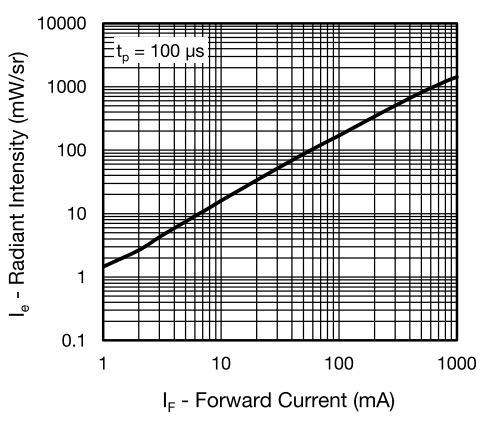
\includegraphics[width=0.6\textwidth]{Figures/ledintensity.png}
  \caption[TSAL6100 Radiant Intensity vs. Forward Current \citep{Vishay2014}]{TSAL6100 Radiant Intensity vs. Forward Current \citep{Vishay2014}}
  \label{fig:ledintensity}
\end{figure}
As the used LEDs require around 200 mA and the selected Arduino\texttrademark board can only provide up to 40 mA, a MOSFET or transistor is needed to control every LED with the Arduino. To avoid having 16 separate integrated circuits, an array should be used.\\
The selected transistor is the ULN2803A Darlington Transistor Array, which allows up to 500 mA peak collector current and an input voltage up to 30 V. Related to its switching characteristics, it has a propagation delay time of 130 ns for low to high level output and 20 ns for high to low level output, which is fast enough to generate the required 56 kHz modulation. In order to save space, a SOIC package will be used. The transistor in the selected package has an acquisition cost of \euro{0.8}.\\

To avoid oscillations due to the 56 kHz oscillation, as well as to protect the prototype from eventual peaks of tension from the source, a 1000 $\mu$F capacitor is going to be used, which has an acquisition cost of \euro{1.44}.\\

The LEDs' connections are illustrated in figure \ref{fig:IRlight}.\\
\begin{figure}[!htb]
  \centering
  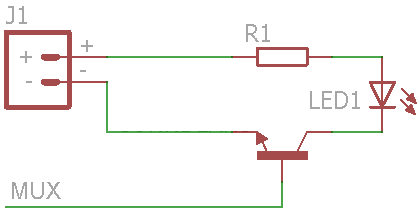
\includegraphics[width=0.4\textwidth]{Figures/EsquemasLights/IRlight.png}
  \caption[Diagram of the TSAL6100 and the ULN2803A Array connections]{Diagram of the TSAL6100 and the ULN2803A Array connections - the array is simplified into a single transistor}
  \label{fig:IRlight}
\end{figure}

As in section \ref{subsection:resistors}, the required resistances can be calculated in order to obtain the correct current in each LED, using easily available resistance values. Knowing that the aircraft used for testing uses a 3S battery (11.1V) and that, for the required forward current of 200 mA, the used LEDs have a forward voltage equal to 1.45 V, as can be seen in figure \ref{fig:irlightcurrent}, we can calculate the correct resistances.\\
\begin{figure}[!htb]
  \centering
  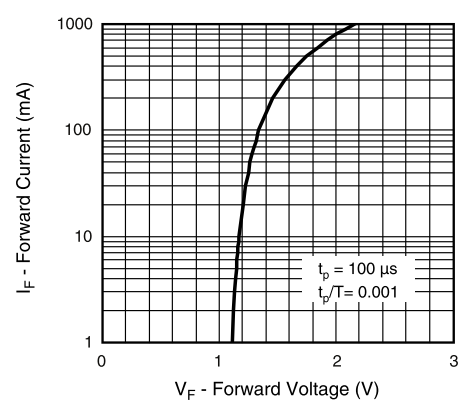
\includegraphics[width=0.6\textwidth]{Figures/irlightcurrent.png}
  \caption[TSAL6100 Forward Current vs Forward Voltage \citep{Vishay2014}]{TSAL6100 Forward Current vs Forward Voltage \citep{Vishay2014}}
  \label{fig:irlightcurrent}
\end{figure}

The voltage drop across each resistor can then be calculated according to equation \eqref{eq:voltagedrop2}.
\begin{equation}\label{eq:voltagedrop2}
V_{D}=V_{S}-V_{F}-V_{T}
\end{equation}
With:
\begin{itemize}
\item $V_{D}$ - Resistor's voltage drop
\item $V_{S}$ - source's voltage
\item $V_{F}$ - LED's forward voltage 
\item $V_{T}$ - Darlington Transistor Array forward voltage
\end{itemize}
According to figures~\ref{fig:IRlight}, the forward voltage for each component is equal to:
\begin{itemize}
\item IR LED - $V_{F} = 1.45 V$
\item ULN2803A Darlington Transistor Array - $V_{T} = 2 V$
\end{itemize}

The obtained value for the correct resistor's voltage drop is equal to 7.65 V. It is then possible to calculate the required resistance with Ohm's law, shown in equation \eqref{eq:ohm2}.
\begin{equation}\label{eq:ohm2}
R=\dfrac{V}{I}
\end{equation}
The obtained resistance is equal to 38.25 $\Omega$. Converting it to the nearest higher rated resistor, in order to use more available material while still protecting the LEDs from too much current, we get 39 $\Omega$. As in section \ref{chapter:passive}, the resistor has an acquisition cost of \euro{0.1}\\

\section{Software}
\label{section:software}

To transmit and receive information with IR frequencies, the IRremote library was adopted. Made by Ken Shirriff, this library allows communication using several IR protocols (such as NEC, Sony's SIRC, Philips RC-5 and RC-6, etc...) \citep{Shirriff2009}.
This library allows the configuration of an Arduino\texttrademark board as a transmitter or as a receiver, with pre-selected IR consumer protocol and frequency. It is also possible to configure the Arduino\texttrademark board as a receiver without specifying the protocol, receiving every signal sent in the receiver's frequency.\\
The IRremote library uses timers to control both the transmission and the reception. For transmission, the timer is programmed to generate PWM at the frequency required for the modulation. For reception, the timer is configured as an interrupt, running the reception code every 50 $\mu$s.\\

The transmitted message, as illustrated in figure \ref{fig:messagecode} is generated by first converting it to binary. This binary is then converted to the RC-5 protocol, with Manchester codification, by turning the timer that generates the PWM modulation on and off to create the necessary high levels and low levels of the message. Finally, the message is transmitted by the IR LEDs.\\
\begin{figure}[!htb]
  \centering
  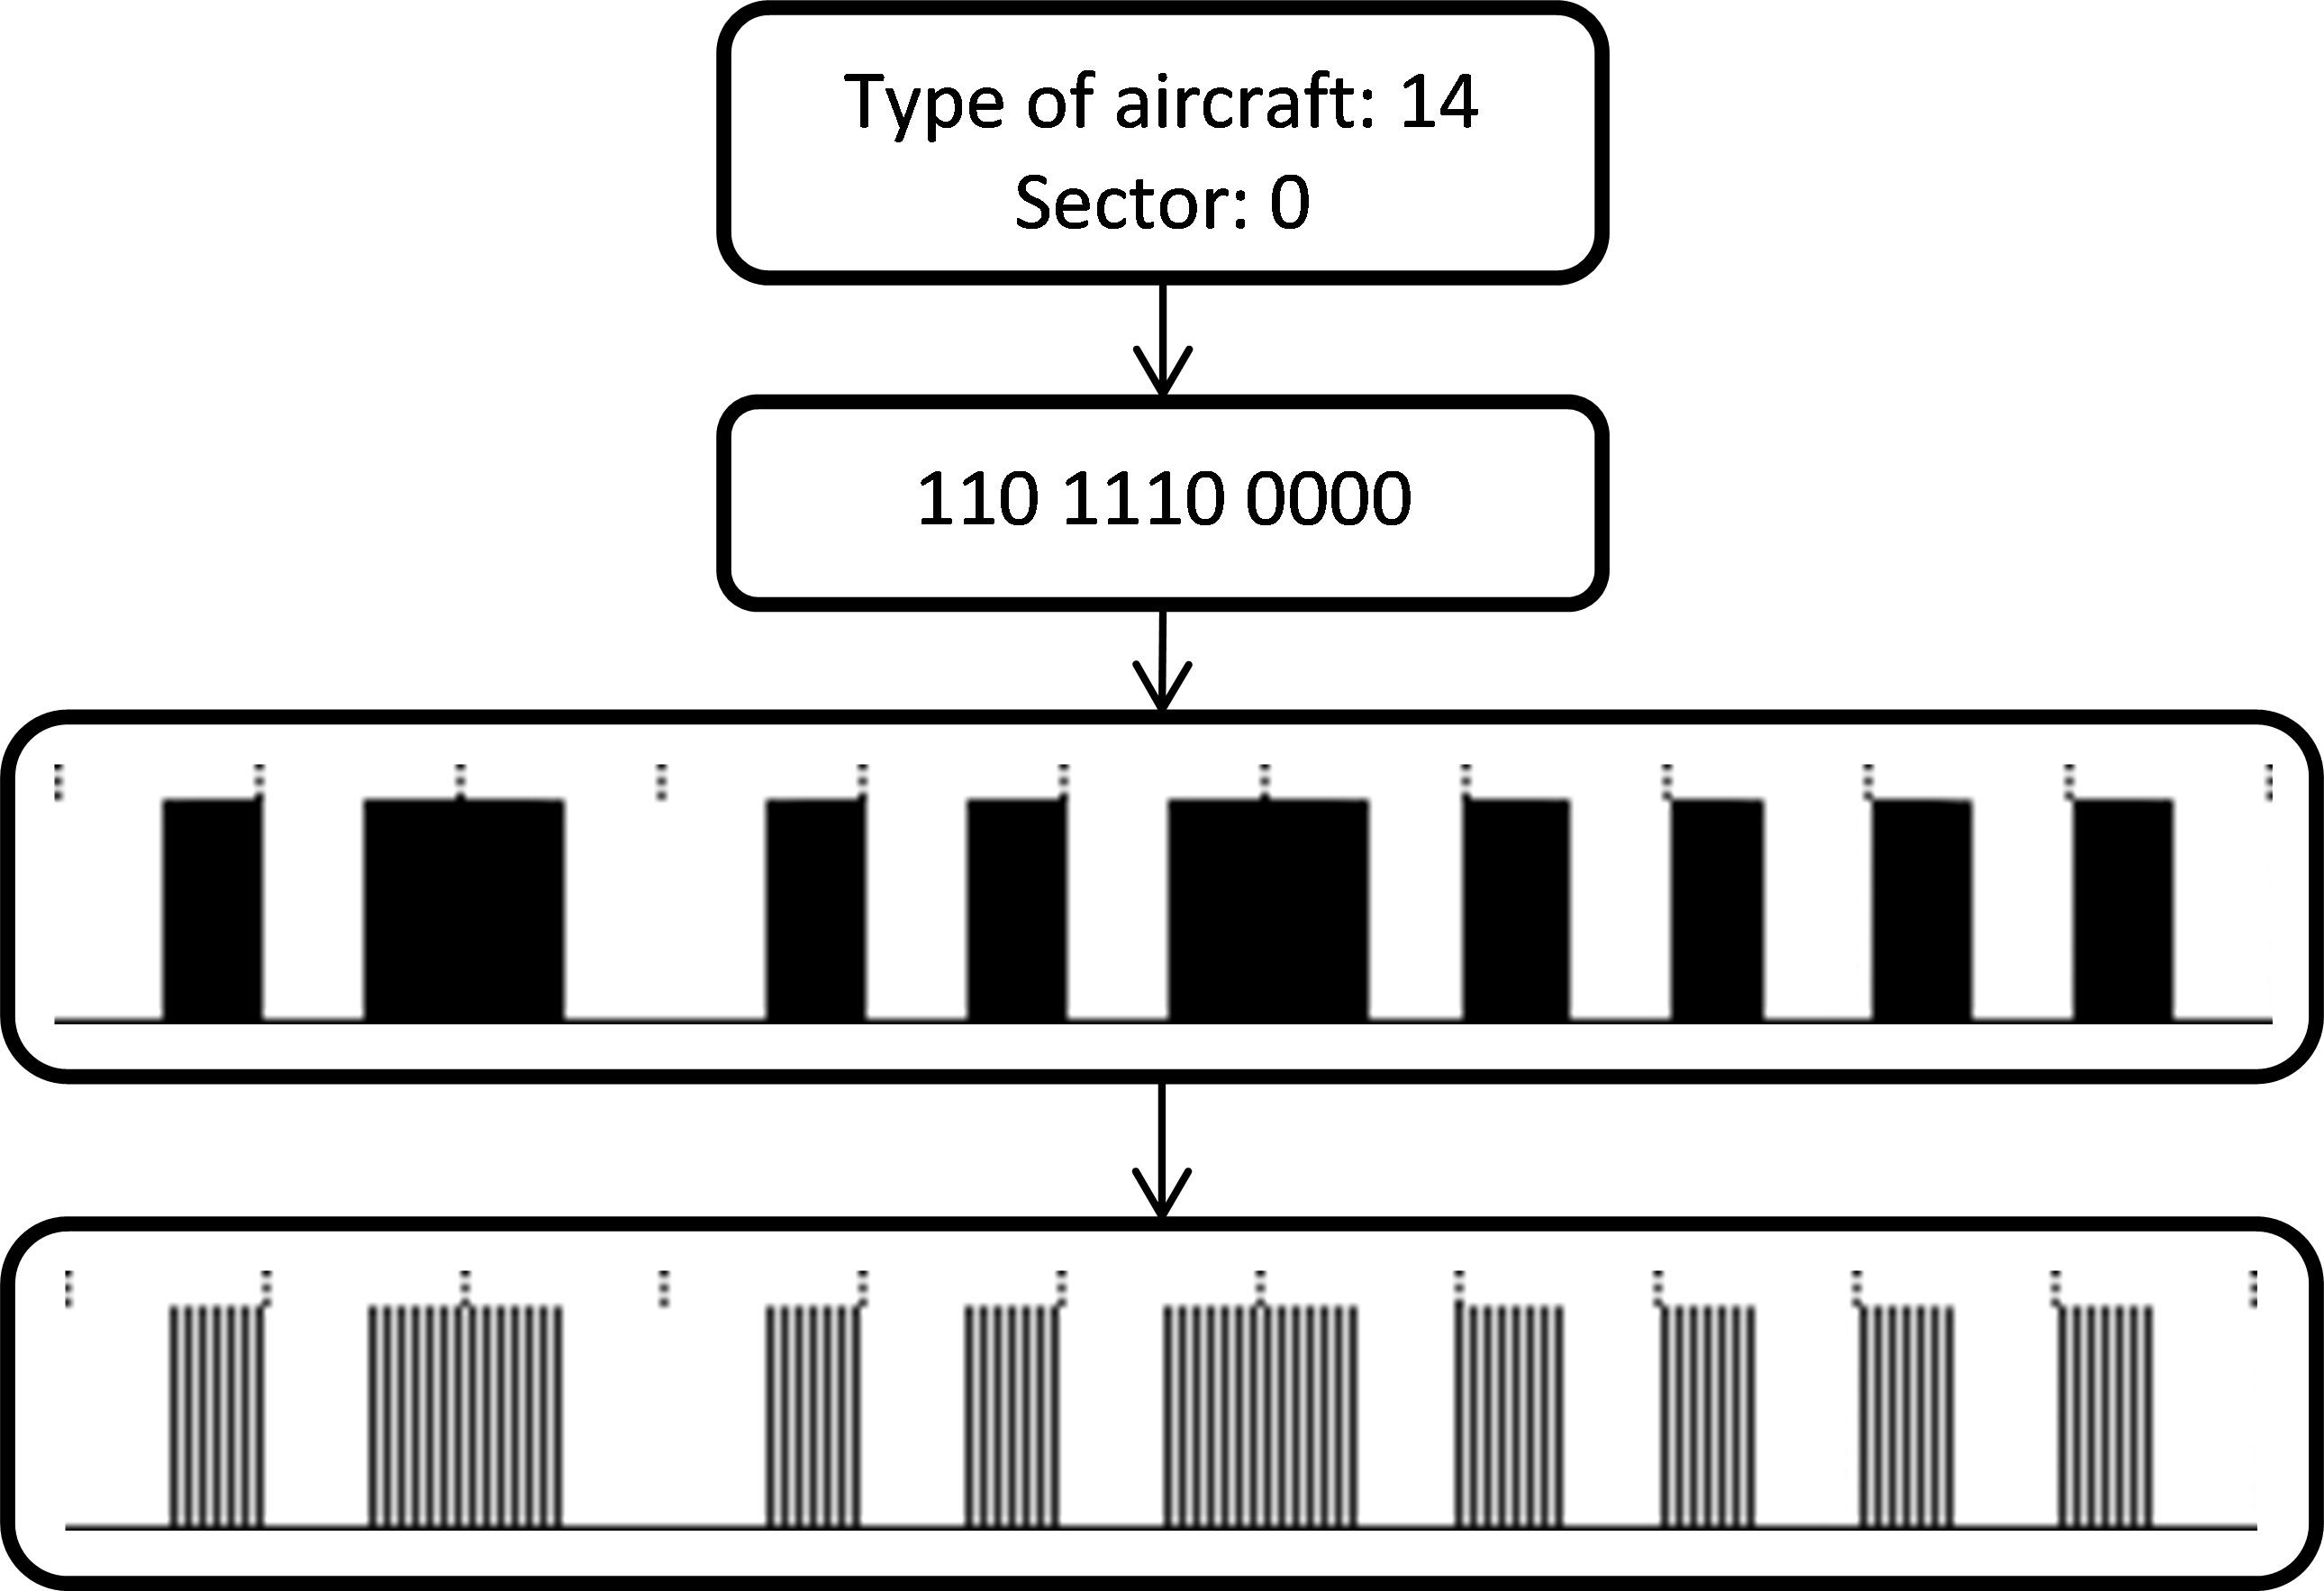
\includegraphics[width=0.8\textwidth]{Figures/messagecode.png}
  \caption[Process of Modulating the Transmitted Message]{Process of Modulating the Transmitted Message - signal not to scale}
  \label{fig:messagecode}
\end{figure}

When receiving, the microcontroller uses a Finite State Machine (FSM) to know which part of the message is expected to receive next. There are four different states, as can be seen in figure \ref{fig:IRspacestate}: Idle, where the microcontroller is waiting for a new message; Stop, in which a message has been fully received and is waiting to be decoded; SPACE, when a low level is being received; and finally MARK, where a high level is being received. The transitions are all represented in figure \ref{fig:IRspacestate}, where variables and functions are represented in lowercase (such as 'irdata' and 'timer') and constants are represented in capital letters ('RAWBUF' and 'GAP\_ TICKS'). The variable 'irdata' contains the received level, 'timer' is used to control the duration of each level, 'rawlen' is the number of entries received since the start of the message and 'decode' is the function that decodes the received message. In the used constants, 'GAP\_ TICKS' is used to control the minimum time between messages, 'RAWBUF' is the maximum length of the duration buffer, 'MARK' represents high level or bit '1' and finally 'SPACE' represents low level or bit '0'.\\
\begin{figure}[!htb]
  \centering
  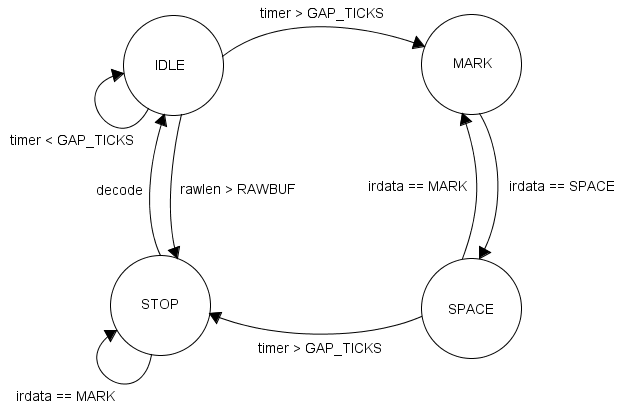
\includegraphics[width=0.9\textwidth]{Figures/IRspacestate.png}
  \caption[IRremote Reception Space State]{IRremote Reception Space State}
  \label{fig:IRspacestate}
\end{figure}

The entire code that allowed the interpretation for all the other protocols, except RC-5, was not needed and it occupied memory as well as processor during run-time, which would delay the reception and transmission of other messages. Because of this, all the unnecessary compiled code was removed.\\

The library was created to enable a single receiver or transmitter. To enable the number required for the prototype, several changes were made.\\
The first, which was necessary to allow several receivers, was to switch the \textit{irparams} structure, that saves everything needed for one receiver, to a vector of structures with length equal to the number of receivers. Then, the reception code was adapted to run for each receiver at a time.\\
The selected Arduino\texttrademark board has three available timers. The original code only used Timer 2 to enable both the transmission and the reception. As the transmission mode requires a timer to generate the PWM signal, while the reception only needs the timer to generate the reception interruptions, the two modes cannot operate with only one timer, or that timer would need to be configured every time it was used. Because Timer 0 is required for all code that manages time (delay, delayMicroseconds, etc...), the transmission was modified to use timer 1, while reception still uses timer 2.\\
As explained in section \ref{subsection:communication}, the signal is modulated using a 56 kHz frequency. The used IRremote library can only modulate signals with frequencies between 36 and 40 kHz, so it was modified for 56 kHz transmission, changing the setup of the timer to allow a faster operation.\\
While Timer 1 can be used to generate the required 56 kHz modulation, it can only output the signal to digital port 9 and so, a multiplexer is required to send the signal to the required 16 IR LEDs. 
By setting the Arduino's digital ports 2 to 5 with the appropriate signal (High or Low), the signal is only transmitted to the selected LED.\\

While studying the timings of the code, it was found that several commands were configuring the same options every cycle. To avoid this, several modifications were made: the configuration of the PWM generating timer (Timer 1) and the direction (output) of the digital ports used for transmission, 2-5 and 9, are now performed only once during the setup function, which only runs when the Arduino is turned on. \\ 

As referred in section \ref{subsection:pcontrolblink}, the Arduino\texttrademark Pro Mini also controls the Anti-Collision Light. The script 'morseaircraft.cpp', has the necessary code and only needs to be called before the setup, to generate the necessary variables (one of them is the type of aircraft in decimal), and once every loop to control the timing of the Morse Code transmitted by the Anti-Collision Light. More information about this script can be found in section \ref{subsection:pcontrolblink}. \\

With the changes stated in section \ref{subsection:solution}, the transmitted message is different from the original RC-5 and so, the transmission and decoding sections also had to be changed. In both sections (function IRsend::sendRC5 for transmission and function IRrecv::decodeRC5), the address bits were removed, the aircraft type was added and the command was replaced with the shorter identification of the transmitting sector.\\

Some important variables were introduced to control important timings in each cycle. The variable 'TX' changes the ratio between number of transmissions and receptions. For example, if 'TX' is 1, for each reception cycle there is one transmission cycle; if 'TX' is 5, there is one transmission cycle in every five reception cycles. 'A' changes the delay between each LED transmission in the same transmission cycle; 'REC' changes the delay before the reception cycle, which gives the receivers more time to receive a complete signal. Finally, there is 'RC5\_ T1' which is equal to half the duration of each transmitted bit. As the used PWM frequency is higher than the original RC-5, the "RC5\_ T1" time can be lowered to allow a higher transmission rate without reducing the number of PWM generated oscillations which are important for a successful reception.

The final code used with the prototype can be seen at https://github.com/MBSFonseca/SenseAndAvoidThesis.\\

\section{Material Testing}
\label{section:materialtesting}

Before building the prototype it was important to check the range and angular view of both the IR LED and the receiver.\\
To test the equipment's range and field of view, a test procedure was created (Test Procedure IR), as seen in section \ref{annex:irmaterial}, which consisted in transmitting several signals between two subsystems, the transmission and the receiver subsystems, at several ranges and angles.\\
%For the test procedure, a schematic was designed for each subsystem. The transmission subsystem, composed by an Arduino\texttrademark Uno, the IR LED, a MOSFET to control the LED with the Arduino\texttrademark, a resistor and a capacitor to control oscillations generated by the PWM signal, was connected according to figure \ref{fig:schematicIR1}. The receiving subsystem, which had the IR receiver, an Arduino\texttrademark Nano and an LED with a resistor that would blink when something was received.\\ , was connected according to figure \ref{fig:schematicIR2}.\\
%\begin{figure}[ht]
%  \centering
%  \subfigure[][]{
%    \label{fig:schematicIR1} 
%    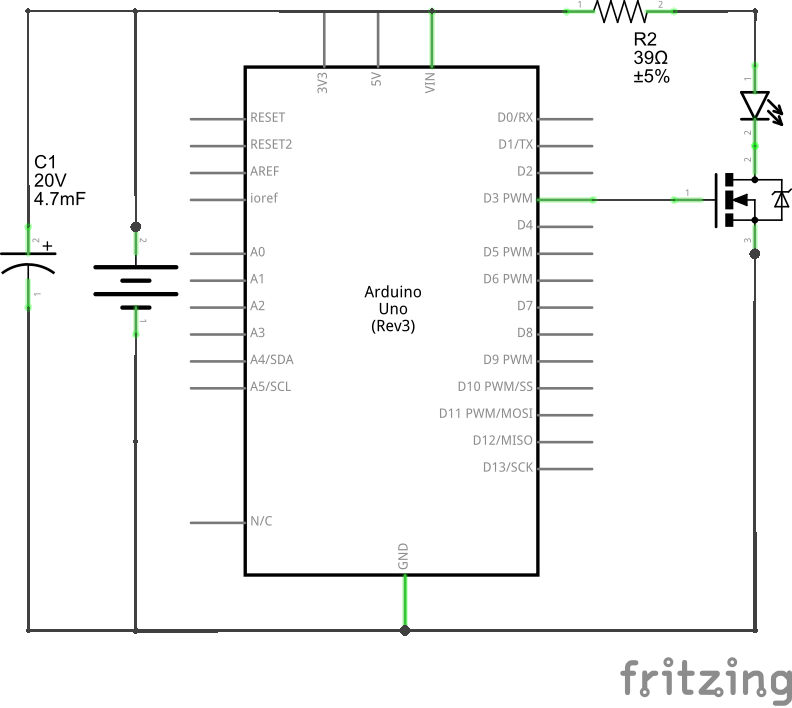
\includegraphics[]{Figures/esquemaled.png}
%  }
%  \hspace{8pt}
%  \subfigure[][]{
%    \label{fig:schematicIR2} 
%    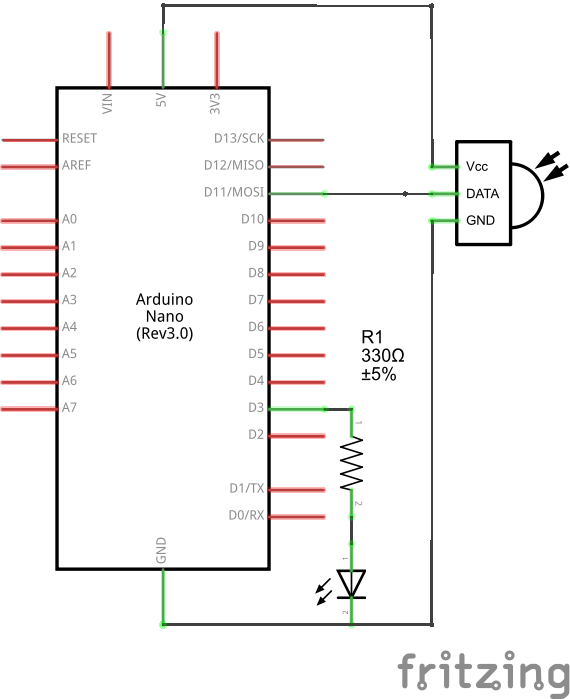
\includegraphics[]{Figures/esquemasensor.png} 
%  }
%  \caption[Schematic Diagram of each Subsystem for Test Procedure]{Schematic diagram of each subsystem for test procedure:
%			\subref{fig:schematicIR1} describes the Transmission subsystem;
%			\subref{fig:schematicIR2} describes the Receiving subsystem.}%
%  \label{fig:schmatics}%
%\end{figure}

The script 'TesteIRreceiver.ino' turns any LED connected to digital port 3 on, when any message is received by the receiver, and outputs the received value to the connected PC.
The script 'TesteIRsender.ino' transmits a message according to the adapted RC-5 protocol every half second. The message, at this time, still contained an address, which was always set to '14', and a command, which may be a '0', a '1' or a '2'.\\
To test the range of both subsystems and the field coverage of the receiving subsystem, an operator would place the transmission equipment on the 'X' mark in figure \ref{fig:ranges1}, and the receiving equipment at the 2 meters mark. After receiving any message, the operator would move the receiving subsystem in the direction of the other marks, perpendicular to the transmitter, until the maximum range was reached. Then the receiving subsystem would be rotated until a maximum angle of reception was reached.\\
\begin{figure}[!htb]
  \centering
  \includegraphics[width=0.70\textwidth]{Figures/ranges1.png}
  \caption[Distances and Positions for both Subsystems for test procedure 1]{Distances and Positions for both Subsystems for range and receiver's field coverage tests}
  \label{fig:ranges1}
\end{figure}

After that, to acquire the transmission subsystem's maximum angular view, the receiving subsystem would be placed in the 'X' mark, as showed in figure \ref{fig:ranges3}, and the transmission subsystem would be moved into the maximum range. A range of 50 m was assumed in the figure. There, the transmission equipment would be rotated until the maximum angular view was reached.\\
\begin{figure}[!htb]
  \centering
  \includegraphics[width=0.70\textwidth]{Figures/ranges3.png}
  \caption[Distances and Positions for both Subsystems for test procedure 2]{Distances and Positions for both Subsystems for transmission's field coverage tests}
  \label{fig:ranges3}
\end{figure}

The tests were repeated during day and nighttime. During daytime, the tests were repeated with a radiation filter on the receiving subsystem to reduce noise generated by the Sun.\\ 

A continuous power provider was used in the transmission subsystem in order to avoid fluctuations on the LEDs' intensity due to PWM oscillations and battery drainage.\\

The results were obtained with the conditions presented in figure \ref{fig:testirconditions}.\\

\begin{figure}[!htb]
  \centering
  \includegraphics[width=1\textwidth]{Figures/testirconditions.png}
  \caption[Conditions during IR test procedure]{Conditions during IR test procedure}
  \label{fig:testirconditions}
\end{figure}

The obtained results are presented in table \ref{tab:irtestsresults}. At night, the range for messages received correctly is 66 m, but it was found that, at 75 m, the receiver still received incomplete data.\\
\begin{table}[]
\centering
\caption{Results for IR test procedure}
\label{tab:irtestsresults}
\begin{tabular}{ccccc}
\hline
                                &              & \multicolumn{2}{c}{Day} & \multirow{2}{*}{Night} \\
                                &              & w/o filter  & w/ filter  &                        \\ \cmidrule(l){3-5}
\multicolumn{2}{c}{Range}                      & 20 m        & 30 m       & 66 m                   \\
\multirow{2}{*}{Field Coverage} & Transmission & 10\degree   & -          & 10\degree              \\
                                & Receiver     & 45\degree   & -          & 45\degree              \\ \hline
\end{tabular}
\end{table}

\section{Prototyping}
\label{section:prototypes}
As presented in section \ref{subsection:solution}, to provide a 360\degree angular coverage, the proposed configuration, showed in figure \ref{fig:irdiagram}, has 16 transmission sectors with one LED each and 4 reception sectors with one receiver each. \\
The first prototype was designed in Fritzing\texttrademark software, and it tried to have every element in a single perforated board. Adding to this, instead of using Darlington Transistor Arrays to control the LEDs, it used MOSFETs, the STB55NF06 in particular, used in the chapter \ref{chapter:passive}.\\ 
%The schematic and board for this prototype can be seen in figure \ref{fig:prototype1}. 
%\begin{figure}[!htb]
%  \centering
%  \subfigure[][]{
%    \label{fig:prototype1schematic} 
%  	\includegraphics[width=0.45\textwidth]{Figures/Prototype1_Esquema.png}
%  }
%  \hspace{8pt}
%  \subfigure[][]{
%    \label{fig:prototype1board} 
%    \includegraphics[width=0.45\textwidth]{Figures/Prototype1_bb.png} 
%  }
%  \caption[First Prototype]{First Prototype:
%			\subref{fig:prototype1schematic} schematic; and,
%			\subref{fig:prototype1board} board.}%
%  \label{fig:prototype1}%
%\end{figure}
%As can be seen in figure \ref{fig:prototype1board}, 
The designed board had to be too wide due to the amount of elements required, with the used MOSFET occupying most of the space. Another problem was the amount of wires required for the connections. As a solution for this problem, a printed circuit was planned but, due to the high number of connections that exited the multiplexer and the Arduino\texttrademark board, the board would have to be double-sided, which is much more complex or expensive to manufacture. Finally the program used to design the board didn't have all the components required and it didn't offer enough tools to correctly position each component.\\

The solution for most problems was to split the equipment into two separate boards: one responsible for transmission and another for reception.\\
Because the previous used program, Fritzing\texttrademark , did not allow to exactly place each element where it was required, a different one was used to design the second version, Eagle\texttrademark .\\

As the prototype is intended to be assembled by each user, it should be easy to manufacture or not expensive to buy already printed. With this in mind, the printed circuit board was designed with thick connections and wide spacing between them, as can be seen in figure \ref{fig:prototype2}.\\
\begin{figure}[!htb]
  \centering
  \subfigure[][]{
    \label{fig:transmitterboard} 
    \includegraphics[width=0.45\textwidth]{Figures/transmitterboard.png}
  }
  \hspace{8pt}
  \subfigure[][]{
    \label{fig:receiverboard} 
    \includegraphics[width=0.45\textwidth]{Figures/receiverboard.png}
  }
  \caption[Second Prototype]{Second Prototype:
			\subref{fig:transmitterboard} transmitter board; and,
			\subref{fig:receiverboard} receiver board.}%
  \label{fig:prototype2}%
\end{figure}

Both boards were printed and the excess copper removed using iron chloride, as shown in figure \ref{fig:pcbmaking}. There were some problems with connections that did not transfer to the copper, and so some connections had to be tinned.\\
%Even so, there were some difficulties found during manufacture:
%\begin{itemize}
%\item A laser printer is required
%\item First board designed with the selected software (Eagle\texttrademark )
%\item Printer's software changed the size of the board
%\item Correctly drill the required holes
%\item Soldering SMDs
%\item Cables used to connect boards were too thick and rigid
%\item Several printed connections did not transfer correctly to copper and disappeared 
%\end{itemize}

\begin{figure}[!htb]
  \centering
  \subfigure[][]{
    \label{fig:pcbcopper} 
    \includegraphics[width=0.3\textwidth]{Figures/pcb2.png}
  }
  \hspace{8pt}
  \subfigure[][]{
    \label{fig:pcbacid1} 
    \includegraphics[width=0.3\textwidth]{Figures/pcb1.png} 
  }\\
  \subfigure[][]{
    \label{fig:pcbacid2} 
    \includegraphics[width=0.3\textwidth]{Figures/pcb4.png}
  }
  \hspace{8pt}
  \subfigure[][]{
    \label{fig:pcbend} 
    \includegraphics[width=0.3\textwidth]{Figures/pcb5.png} 
  }
  \caption[PCB printing process]{PCB printing process:
			\subref{fig:pcbcopper} printed image transferred to copper;
			\subref{fig:pcbacid1} iron chloride reacting with copper;
			\subref{fig:pcbacid2} iron chloride reacting with copper; and,
			\subref{fig:pcbend} finished boards.}%
  \label{fig:pcbmaking}%
\end{figure}

After finishing the boards, the elements were soldered with special attention to the SMD components, the cables that connect the boards were manufactured and two prototypes were assembled, as shown in figure \ref{fig:twoprototypes}.\\
\begin{figure}[!htb]
  \centering
  \includegraphics[width=0.8\textwidth]{Figures/twoprototypes.png}
  \caption[Finished prototypes]{Finished prototypes}
  \label{fig:twoprototypes}
\end{figure}

To protect the prototypes and to decrease the angular view of the IR receivers, a 3D printed box was created. The box is composed of three parts, so that the prototype can be assembled inside the box.\\
As each receiver is able to receive beyond the angular view of 90\degree , the reception sectors for each receiver were increased to 130\degree . This increase in the angular view creates four virtual sectors, where the signal is received by two receivers.\\
The technical drawings of the created design can be seen in \textbf{\# Annex reference here \#}.
After printing, the pieces were also painted black.\\
The final result can be seen in figures~\ref{fig:printedbox2}--\subref{fig:printedbox3}.\\

\begin{figure}[!htb]
  \centering
  \subfigure[][]{
    \label{fig:printedbox2} 
    \includegraphics[width=0.45\textwidth]{Figures/printedbox2.png}
  }
  \hspace{8pt}
  \subfigure[][]{
    \label{fig:printedbox3} 
    \includegraphics[width=0.45\textwidth]{Figures/printedbox3.png} 
  }\\
  \caption[3D Printed Box]{3D printed box:
			\subref{fig:printedbox2} printed parts; and,
			\subref{fig:printedbox3} assembled box.}%
  \label{fig:printedbox}%
\end{figure}

The assembled product is shown in figures~\ref{fig:irprototype1}--\subref{fig:irprototype2}.\\

\begin{figure}[!htb]
  \centering
  \subfigure[][]{
    \label{fig:irprototype1} 
    \includegraphics[width=0.45\textwidth]{Figures/irprototype1.png}
  }
  \hspace{8pt}
  \subfigure[][]{
    \label{fig:irprototype2} 
    \includegraphics[width=0.45\textwidth]{Figures/irprototype2.png} 
  }\\
  \caption[Assembled IR Sense and Avoid Prototype]{Assembled IR sense and avoid prototype:
			\subref{fig:irprototype1} top view; and,
			\subref{fig:irprototype2} side view.}%
  \label{fig:irprototype}%
\end{figure}

The total acquisition cost is \euro{37,54} which include \euro{10} for miscellaneous items, such as cables, connectors and plastic for the printed box.\\

\subsection{ISR's quadcopter}
\label{subsection:IRpisr}
The created prototype was then adapted to a quadcopter. \\
The used quadcopter has a Nvidia Jetson Tk1 onboard, which is responsible for the high level control. This board would be responsible to avoid collisions, receiving data from the prototype through USB serial communication.\\
The only required connections between the aircraft and the prototype are a USB serial port, used to establish communication between the prototype and the Nvidia board, and two cables connected to the aircraft's power distribution board in order to power up the prototype.\\
The quadcopter can be seen in figure \ref{fig:irprototype3} with the prototype fixed on top.\\

\begin{figure}[!htb]
  \centering
  \includegraphics[width=0.6\textwidth]{Figures/irprototype3.png}
  \caption[IR Sense and Avoid Prototype Assembled on Quadcopter]{IR sense and avoid prototype assembled on quadcopter}
  \label{fig:irprototype3}
\end{figure}

\section{Prototype Testing}
\label{section:prototypetest}
\subsection{Time Variables Optimization}
\label{subsection:opt}
Before testing the prototypes, the four variables ('TX', 'A', 'REC' and 'RC5\_ T1') that control important times in each cycle had to be optimized. To do this, an automatic test was designed. Two prototypes would run the given values for 60 seconds and the number of receptions during each test would be saved.\\
As the variable 'RC5\_ T1' can not be changed without compiling the code, the test would only change the other three variables, with the 'RC5\_ T1' being changed by hand between tests.\\
Each prototype would be connected to a different computer and laboratory power supplies, and would be place 10 m apart without obstacles between them.  The developed code would be loaded into each Arduino\texttrademark board, so that the prototype would wait for the variables that each pc would send. After the setup cycle, the code is equal to the normal Sense and Avoid prototype.\\

To enable synchronization between both prototypes, a Socket server and client were developed in Python. One computer would run the server and the other the client.\\
The server script waits to receive 'TX', 'A' and 'REC' from the client and then sends this information to the connected prototype. It then allows the prototype to run normally until the client tells him to stop and sends the new values for the variables, which the server then sends to the prototype again. In the client side, the script first changes the tested variables, sending them to the server and to its connected prototype. After one minute, it stops the communication with the prototype, tells the server to do the same, saves the variables' values and the number of receptions into a file and starts again with different values.\\

The tested values were:
\begin{itemize}
\item 'TX' - 1, 5, 10, 15, 20
\item 'A' - 1, 3, 5, 10
\item 'REC' - 10, 20, 40, 60, 100
\item 'RC5\_ T1' - 100, 200, 300, 500, 700, 889
\end{itemize}

\subsection{Blind zones}
\label{subsection:blindzones}
In order to check if the prototypes had blind zones in transmission or reception, a test was prepared.\\
To check for blind zones in transmission, both prototypes are set on tripods to avoid reflections from the ground. Then, one prototype is connected to the PC and battery, while the second prototype is placed at the tested distance, only connected to the battery, and is able to rotate. With both prototypes working, the second prototype is rotated in 5\degree intervals, with a pause of 5 seconds between rotation, until the 360\degree are reached. At the end, the number of receptions shows the angular transmission quality.\\

To check for blind zones in reception, both prototypes are set on tripods to avoid reflections from the ground. Then, one prototype is connected to the PC and battery, while the second prototype is placed at the tested distance, only connected to the battery. With both prototypes working, the first prototype, which is connected to the PC, is rotated in 5\degree intervals, with a pause of 5 seconds between rotation, until the 360\degree are reached. At the end, the number of receptions shows the angular reception quality.\\

The tests were repeated at ranges of 7, 9 and 11 meters.\\

\subsection{Ranges}
\label{subsection:ranges}
In order to check the maximum range of the prototype, a test procedure was designed.\\
With one prototype fixed, the other would move away in a straight line, perpendicularly to the fixed prototype, until the maximum range was found. The test would be repeated during day and nighttime, inside a building and outside.\\ 

As it was found that the receivers would saturate with the selected resistors, due to high radiant intensity, another two resistors with lower resistances (56 and 82 $\Omega$) were tested indoors during daytime.\\
Using equation \eqref{eq:ohm2} and figure \ref{fig:ledintensity} again, we can calculate the LED's forward current and radiant intensity with the new resistors. The results are shown in table \ref{tab:ledintensity2}.\\
\begin{table}[]
\centering
\caption[Forward Current and Radiant Intensity of IR LED with new Resistors]{Forward Current and Radiant Intensity of IR LED with new Resistors}
\label{tab:ledintensity2}
\begin{tabular}{@{}ccc@{}}
\toprule
                     & Forward Current (mA) & Radiant Intensity (mW/sr) \\ \cmidrule(l){2-3}
56 $\Omega$ Resistor & 136.6                & 200                       \\
82 $\Omega$ Resistor & 93.3                 & 150                       \\ \bottomrule
\end{tabular}
\end{table}

Adding to this, a filter was applied to the receivers to reduce ambient noise and the tests were repeated.\\

\subsection{Maneuvers}
\label{subsection:maneuvers}
In order to test the designed prototypes in important situations for collision avoidance, a test procedure was planned, as can be seen in section \ref{annex:maneuvers}.\\
Several configurations would be evaluated, as shown in figures~\ref{fig:configheadon}--\subref{fig:configovertaking}, beginning with static tests of each situation, followed by non-static tests which tried to simulate the correct avoidance maneuvers for each situation.\\ 

\begin{figure}[!htb]
  \centering
  \subfigure[][]{
     \includegraphics[width=0.25\textwidth]{Figures/VL-Rules3.jpg}
     \label{fig:configheadon}
  }\hspace{3pt}
  \subfigure[][]{
     \includegraphics[width=0.33\textwidth]{Figures/VL-Rules4.jpg}
     \label{fig:configconverging}
  }\hspace{3pt}
  \subfigure[][]{
     \includegraphics[width=0.25\textwidth]{Figures/VL-Rules5.jpg}
     \label{fig:configovertaking}
  }\\
  \caption[Maneuvers Test's Configurations \citep{Planefinder2012}]{Maneuvers Test's Configurations \citep{Planefinder2012}:
			\subref{fig:configheadon} - head on approach;
			\subref{fig:configconverging} - converging approach; and,
			\subref{fig:configovertaking} - overtaking approach.}%
  \label{fig:configurations}
\end{figure}

\subsection{ISR drone}
\label{subsection:IRisrdrone}

In order to test the designed prototypes with an aircraft, a test procedure was planned, which can be seen in section \ref{annex:sas}.\\
The same configurations of section \ref{subsection:maneuvers} would be tested.\\ 

The Nvidia on-board the aircraft was programmed to start a serial communication with the prototype at start up, and log all the data received into a file with the time stamp.\\
As a first test, one prototype would be fixed on top of a quadcopter and the other placed on top of a tripod. The aircraft would then move as described in the test procedure, so that detection data would be stored.\\
Due to time restrictions and problems with the used quadcopter's batteries, the test could not be successfully completed and no results were collected.\\
 % file "Thesis_ActiveSolution.tex"

%%%%%%%%%%%%%%%%%%%%%%%%%%%%%%%%%%%%%%%%%%%%%%%%%%%%%%%%%%%%%%%%%%%%%%%%
%                                                                      %
%     File: Thesis_Results.tex                                         %
%     Tex Master: Thesis.tex                                           %
%                                                                      %
%     Author: Andre C. Marta                                           %
%     Last modified : 21 Jan 2011                                      %
%                                                                      %
%%%%%%%%%%%%%%%%%%%%%%%%%%%%%%%%%%%%%%%%%%%%%%%%%%%%%%%%%%%%%%%%%%%%%%%%

\chapter{Results and Discussion}
\label{chapter:results}

\section{Visible Spectrum Solution's Results}
\label{section:passiveresults}

The tests were performed in bright daylight. As stated in section \ref{section:pmaterialtesting}, half the individuals started at the 350 m mark and the other half at 50 m. The study was conducted with around 67\% pilots. All subjects were between 18 and 25 years old.\\
The obtained results for each light are shown in figure \ref{fig:statistic} with the top and lower whiskers identifying the maximum and minimum evaluation respectively, the green block identifying the first quartile and the violet block (only seen in figure \ref{fig:statisticanti}) representing the third quartile. The band between the green and violet blocks identifies the median. \\
\begin{figure}[!ht]
  \centering
  \subfigure[][]{
    \label{fig:statisticleft} 
    \includegraphics[width=0.45\textwidth]{Figures/Statistics/LeftPosition.png}
  }
  \hspace{8pt}
  \subfigure[][]{
    \label{fig:statisticright} 
    \includegraphics[width=0.45\textwidth]{Figures/Statistics/RightPosition.png} 
  }\\
  \subfigure[][]{
    \label{fig:statisticrear} 
    \includegraphics[width=0.45\textwidth]{Figures/Statistics/RearPosition.png}
  }
  \hspace{8pt}
  \subfigure[][]{
    \label{fig:statisticanti} 
    \includegraphics[width=0.45\textwidth]{Figures/Statistics/AntiCollision.png} 
  }
  \caption[Statistic Study Results]{Statistic study results for each light:
			\subref{fig:statisticleft} left position;
			\subref{fig:statisticright} right position;
			\subref{fig:statisticrear} rear position; and,
			\subref{fig:statisticanti} anti-collision.}%
  \label{fig:statistic}%
\end{figure}
As can be seen, specially in figures~\ref{fig:statisticleft}--\subref{fig:statisticrear}, the maximum distance was not far way enough to achieve a high decline. Even so, it is clear that the anti-collision achieves the worst result, with a big difference to the left position light, followed by the right and finally the rear position light. The anti-collision has a much higher angular coverage, so the lower range was expected. Adding to this, although the light was still quite clear at the 350 meters mark, the Morse code was not so perceptible which caused several subjects to decrease their grade.\\

\section{Infrared Solution's Results}
\label{section:activeresults}
\subsection{Time Variables Optimization Results}
\label{subsection:optresults}
The results from tests in section \ref{subsection:opt} are presented below.\\
The total number of receptions for each variable is represented in figure \ref{fig:optresults1}. 
The best result for the variable 'TX', expressed in figure \ref{fig:opttx}, is for value 5, while value 1 presents the worst case. The low number of receptions when 'TX' is equal to 1 might be caused by the high percentage of time each system spends transmitting, which is not spent in reception. On the other hand, too much time without transmitting any message also decreases the number of receptions, as can be seen with the increase of 'TX' to 10, 15 and 20.\\
For variable 'A', in figure \ref{fig:opta}, there is a big decrease in receptions between values 1 and 3, followed by an incremental rise until the maximum is reached at value 10. \\
For variable 'REC', showed in figure \ref{fig:optrec}, the maximum is achieved with the lowest value, 10, with a gradual decrease of the number of receptions for larger values of the variable.\\
Finally, variable 'RC5\_ T1', which defines the duration of each level (high or low) inside the transmitted message, has zero receptions for value 100, increasing until the maximum is reached at value 700 and then decreasing at value 889, which is the standard for the RC-5 protocol, as presented in figure \ref{fig:optrc5}. The increase of the modulation frequency to 56 kHz allows a slight decrease of variable 'RC5\_ T1' from 889 to 700, which increases the transmission rate. For lower values of 'RC5\_ T1' though, the lower duration of the message has an increasing negative impact on the reception rate.\\

\begin{figure}[!ht]
  \centering
  \subfigure[][]{
    \label{fig:opttx} 
    \includegraphics[width=0.40\textwidth]{Figures/Optimization/tx.png}
  }
  \hspace{8pt}
  \subfigure[][]{
    \label{fig:opta} 
    \includegraphics[width=0.40\textwidth]{Figures/Optimization/a.png} 
  }\\
  \subfigure[][]{
    \label{fig:optrec} 
    \includegraphics[width=0.40\textwidth]{Figures/Optimization/rec.png}
  }
  \hspace{8pt}
  \subfigure[][]{
    \label{fig:optrc5} 
    \includegraphics[width=0.40\textwidth]{Figures/Optimization/rc5.png} 
  }
  \caption[Optimization Test Results for each Variable]{Optimization test results for each variable:
			\subref{fig:opttx} 'TX';
			\subref{fig:opta} 'A';
			\subref{fig:optrec} 'REC'; and,
			\subref{fig:optrc5} 'RC5\_ T1'.}%
  \label{fig:optresults1}%
\end{figure}

The charts shown in figure~\ref{fig:optresults2} illustrate the evolution of the controlled variables when other is changed. Starting with figures~\ref{fig:opttxrc5}--\subref{fig:optrecrc5} which show the relation between the variable 'RC5\_ T1' and the other three, while figure~\ref{fig:opttxa} shows the relation between 'TX' and 'A', figure~\ref{fig:opttxrec} the relation between 'TX' and 'REC', and finally figure~\ref{fig:optarec} shows the variables 'A' and 'REC'.\\

\begin{figure}[!ht]
  \centering
  \subfigure[][]{
    \label{fig:opttxrc5} 
    \includegraphics[width=0.45\textwidth]{Figures/Optimization/txrc5.png}
  }
  \hspace{8pt}
  \subfigure[][]{
    \label{fig:optarc5} 
    \includegraphics[width=0.45\textwidth]{Figures/Optimization/arc5.png} 
  }\\
  \subfigure[][]{
    \label{fig:optrecrc5} 
    \includegraphics[width=0.45\textwidth]{Figures/Optimization/recrc5.png}
  }
  \hspace{8pt}
  \subfigure[][]{
    \label{fig:opttxa} 
    \includegraphics[width=0.45\textwidth]{Figures/Optimization/txa.png} 
  }\\
  \subfigure[][]{
    \label{fig:opttxrec} 
    \includegraphics[width=0.45\textwidth]{Figures/Optimization/txrec.png}
  }
  \hspace{8pt}
  \subfigure[][]{
    \label{fig:optarec} 
    \includegraphics[width=0.45\textwidth]{Figures/Optimization/arec.png} 
  }
  \caption[Optimization Test Results - Relations between Variables]{Optimization test results - relations between variables:
			\subref{fig:opttxrc5} relation between 'TX' and 'RC5\_ T1';
			\subref{fig:optarc5} relation between 'A' and 'RC5\_ T1';
			\subref{fig:optrecrc5} relation between 'REC' and 'RC5\_ T1';
			\subref{fig:opttxa} relation between 'TX' and 'A';
			\subref{fig:opttxrec} relation between 'TX' and 'REC'; and,
			\subref{fig:optarec} relation between 'A' and 'REC'.}%
  \label{fig:optresults2}%
\end{figure}

As can be seen in figures~\ref{fig:opttxrc5}--\subref{fig:optrecrc5}, the optimum value for the variable 'RC5\_ T1' is between 500 and 700, with a clear maximum in figure~\ref{fig:opttxrc5} for 700.\\
For variable 'TX', it is clear that value 1 gives the worst results, with zero receptions. For maximum receptions, the variations are not so clear with only a slight decrease in the number of receptions as we increased 'TX'.\\
As can be seen in figures~\ref{fig:optarc5}, \subref{fig:opttxa} and \subref{fig:optarec}, variable 'A' has the minimum number of receptions for value 3, with a clear increase for value 1 and for higher values. Overall, the higher number of receptions were achieved for value 10.\\
Finally, the variable 'REC' shows a clear decrease in receptions for higher values, with the highest number of receptions achieved for the minimum value 10.\\

Although there is no perceptible influence in the results, each test was not run under the same ambient light conditions, as the total time for the optimization test surpassed 12 hours and the room could not be blacked out during daytime.\\

The chosen values for the variables were:
\begin{itemize}
\item 'TX' - 5
\item 'A' - 10
\item 'REC' - 10
\item 'RC5\_ T1' - 700
\end{itemize}

\subsection{Blind Zone Results}
\label{subsection:blindzoneresults}
The results for tests in section \ref{subsection:blindzones} are shown in figure \ref{fig:blind}.\\

\begin{figure}[!ht]
  \centering
  \subfigure[][]{
    \label{fig:blinde7} 
    \includegraphics[width=0.4\textwidth]{Figures/teste7m.png}
  }
  \hspace{8pt}
  \subfigure[][]{
    \label{fig:blindr7} 
    \includegraphics[width=0.4\textwidth]{Figures/receptor7m.png} 
  }\\
  \subfigure[][]{
    \label{fig:blinde9} 
    \includegraphics[width=0.4\textwidth]{Figures/teste9m.png}
  }
  \hspace{8pt}
  \subfigure[][]{
    \label{fig:blindr9} 
    \includegraphics[width=0.4\textwidth]{Figures/receptor9m.png} 
  }\\
  \subfigure[][]{
    \label{fig:blinde11} 
    \includegraphics[width=0.4\textwidth]{Figures/teste11m.png}
  }
  \hspace{8pt}
  \subfigure[][]{
    \label{fig:blindr11} 
    \includegraphics[width=0.4\textwidth]{Figures/receptor11m.png} 
  }
  \caption[Blind Zones Test Results]{Blind zones test results:
			\subref{fig:blinde7} transmission at 7 m;
			\subref{fig:blindr7} reception at 7 m;
			\subref{fig:blinde9} transmission at 9 m;
			\subref{fig:blindr9} reception at 9 m;
			\subref{fig:blinde11} transmission at 11 m; and,
			\subref{fig:blindr11} reception at 11 m.}%
  \label{fig:blind}%
\end{figure}

As a first analyzes to figures \ref{fig:blinde7}, \subref{fig:blinde9} and \subref{fig:blinde11}, the low reception rates in some sectors, for example sector 1 (22.5\degree ) in figures \ref{fig:blinde9} and \subref{fig:blinde11}, may be explained by the incorrect positioning of the LED of that sector, with it pointing upwards or downwards instead of horizontally. Adding to this, there are some LEDs which may be pointed towards other sectors, such as LED 0 in figure \ref{fig:blinde7} which should have more receptions at 0\degree and 5\degree . Other possible justification for this is the incorrect rotation of the transmitting prototype during tests.\\

Then, considering a blind zone in transmission when the number of receptions is under 3 for a distance of 7 m, under 2 for 9 m and equal to 0 for 11 m, we have the following blind zones:
\begin{itemize}
\item At 7 m, there are blind zones of 15\degree between sectors 0/1, 4/5, 6/7 and 12/13; the rest of areas between sectors all have 10\degree blind zones except between sectors 13/14 which is only of 5\degree .
\item At 9 m, there are no blind zones of 15\degree , but most areas have blind zones of 10\degree , except between sectors 2/3, 3/4, 5/6, 8/9, 9/10, 10/11 and 15/0 which have blind zones of only 5\degree .
\item At 11 m, there is only one blind zone of 10\degree between sector 1 and 2, which may be caused by LED1 being incorrectly pointed. All the other areas between LEDs have blind zones of 5\degree except for areas between sectors 8/9, 9/10, 11/12, 13/14 and 14/15 which do not have blind zones.
\end{itemize}

For the reception blind zones at 7 m range, in figure \ref{fig:blindr7} we can see that there is no clear blind zone, only a reduction in the number of receptions on a 5\degree sector which belongs to receiver 0.\\
For the 9 m test, there are a couple blind zones between each receiver, at approximately 45, 135, 225 and 315\degree .\\
Finally, at 11 meters, the reception rate was much lower, with several zones only receiving two times. Nonetheless, it is possible to see an increase of receptions when the transmitter is in front of a receiver or between two, with each receiver receiving mostly at different times.\\

Analyzing the data from the reception blind zones test, it is possible to see that the virtual sectors do not work properly, as it is impossible to guaranty that both receivers are receiving the signal at the same time. Because of this, only 50\% of the received signals in a virtual sector were received by two receivers (data not represented in figure \ref{fig:blind}).\\

\subsection{Ranges' results}
\label{subsection:rangesresults}
Results for tests in section \ref{subsection:ranges}.\\
The results for the tests done indoors are shown in table \ref{tab:ranges}.
\begin{table}[!ht]
\centering
\caption[Results for Indoor Range Tests]{Results for indoor range tests}
\label{tab:ranges}
\begin{tabular}{@{}cccccccc@{}}
\toprule
                     &       & \multicolumn{2}{c}{39$\Omega$} & \multicolumn{2}{c}{56$\Omega$} & \multicolumn{2}{c}{82$\Omega$} \\ \cmidrule(l){3-8} 
                     &       & w/ Filter   & w/o Filter       & w/ Filter   & w/o Filter       & w/ Filter   & w/o Filter       \\
\multirow{2}{*}{Max} & Day   & 20          & \textgreater50   & 15.2        & \textgreater50   & 13.8        & \textgreater50   \\
                     & Night & 24.7        & \textgreater50   & -           & -                & -           & -                \\
\multirow{2}{*}{Min} & Day   & 4.5         & 11.5             & 3.8         & 10               & 3        	 & 9.1 \\
                     & Night & 6.5         & 17               & -           & -                & -           & -                \\ \hline
\end{tabular}
\end{table}

As expected, the use of higher resistance decreased the minimum and maximum ranges, due to the lower radiance intensity. Adding to this, the absence of a filter has a high effect on the ranges, with the receivers saturating at longer distances, but also increasing the maximum range. The difference in the minimum distances between day and night is due to the receiver's automatic gain control, which adjusts the irrandiance threshold for different ambient noise.\\
The maximum ranges were also tested outdoors. During daytime, the maximum ranges achieved were 26 m with 39 $\Omega$, 21.5 m with 56 $\Omega$ and 13.6 m with 82 $\Omega$. During nighttime the only resistance tested was 39 $\Omega$, which gave a range of 62 m.\\

\subsection{Maneuvers' Results}
\label{subsection:maneuversresults}
The results for the tests done in section \ref{subsection:maneuvers} are presented bellow.\\
\subsubsection{Static tests}
The first conducted tests were static, in order to confirm that both prototypes were working as expected.\\
In the head-on position, both aircraft detected a threat, receiving transmission sector 0 in reception sector 0.\\
Next, in the converging position, both aircraft also detected a threat, with aircraft 1 receiving transmission sector 14 in reception sectors 0 and 1, and aircraft 2 receiving transmission sector 2 in reception sectors 0 and 3.\\
Finally, in overtaking position, aircraft 1 received the transmission sector 8 in reception sector 0, and aircraft 2 transmission sector 0 in reception sector 2, as was expected.\\

After making sure that both prototypes were producing the correct detection, several maneuvers were tested and which results are presented bellow.\\
\subsubsection{Head-on collision avoidance maneuver}
The results for aircraft 1, from figure \ref{fig:configheadon}, in the head-on collision avoidance maneuver are shown in figure \ref{fig:resultsheadon}. The graphic shows the receptions for each receiver, as well as the threat's transmitting sector (over the mark) whenever it changes. The messages received by two receivers at the same time (virtual sectors) are represented between them, for example, the data that receivers 2 and 3 received at 15:56:51 is represented between these receivers.\\

\begin{figure}[!ht]
  \centering
  \includegraphics[width=1\textwidth]{Figures/Maneuvers/headon.png}
  \caption[Results for Head-On Collision Avoidance Maneuver]{Results for head-on collision avoidance maneuver}
  \label{fig:resultsheadon}
\end{figure}

As can be read in section \ref{annex:maneuvers}, this maneuver consisted on simulating a head-on collision avoidance maneuver, where each aircraft must move to its right, until a safe separation distance is reached.\\
Although some errors are visible in the data, the results are consistent with what was expected with a possible head-on collision being detected, followed by a right turn at 15:56:09 to avoid collision. When aircraft 1 is almost behind the threat, at 15:57:03, it turns left to return to its flight path. It is also possible to see that the intruder (aircraft 2) turned right before aircraft 1, at 15:56:07, as the received messages switch from a 0 to a 14.\\

\subsubsection{Converging collision avoidance maneuver}
The results for aircraft 1, from figure \ref{fig:configconverging}, in the converging collision avoidance maneuver are shown in figure \ref{fig:resultsconverging}. The graphic has the same format as figure \ref{fig:resultsheadon}.\\

\begin{figure}[!ht]
  \centering
  \includegraphics[width=1\textwidth]{Figures/Maneuvers/converging.png}
  \caption[Results for Converging Collision Avoidance Maneuver]{Results for converging collision avoidance maneuver}
  \label{fig:resultsconverging}
\end{figure}

As can be read in section \ref{annex:maneuvers}, this maneuver consisted on simulating a converging collision avoidance maneuver, where aircraft 1 (the one on the left) must move to its right, until a safe separation distance is reached.\\ 
In the graphic it is possible to see that an intruder was at the right side of aircraft 1. After a while, around 16:04:25, aircraft 1 turns to its right and then moves forward. The transmitting sector of the intruder doesn't change until aircraft 1 moves forward at 16:04:36. This tells us that aircraft 1 moved towards aircraft 2, while it should have continued turning right, as the distance and speed of the threat was not known, until aircraft 2 was between sector 0 and 3, to correctly avoid colliding with it. Still, right after aircraft 1 moves forward, it starts receiving a different sector from the threat and, later, the signals arrive at receivers 0 and 3, which means that the threat is now on its left side. When aircraft 1 is behind aircraft 2, at 16:05:16, it turns right and continues on its flight path.\\

\subsubsection{Overtaking collision avoidance maneuver}
The results for aircraft 1, from figure \ref{fig:configovertaking}, in the overtaking collision avoidance maneuver are shown in figure \ref{fig:resultsovertake}. The graphic has the same format as figure \ref{fig:resultsheadon}.\\

\begin{figure}[!ht]
  \centering
  \includegraphics[width=1\textwidth]{Figures/Maneuvers/overtake.png}
  \caption[Results for Overtaking Collision Avoidance Maneuver]{Results for overtaking collision avoidance maneuver}
  \label{fig:resultsovertake}
\end{figure}

As can be read in section \ref{annex:maneuvers}, this maneuver consisted on simulating an overtaking collision avoidance maneuver, where aircraft 1 (the one overtaking) must move to its right, until a safe separation distance is reached.\\
In the graphic it is possible to see aircraft 1 detecting a thread in front of it, and that it is behind the threat. At 16:23:38, aircraft 1 turns right to avoid a collision. Then, when the thread's transmitting sector switches to 6, aircraft 1 turns left to its original destination, as it is clear from the threat.\\

During testing, it was found that the virtual sectors created for reception did not work as predicted. As can be seen in figure \ref{fig:resultsovertake} between 16:23:37 and 16:23:48, the threat switches from sector 0 to 3 and between them multiple times. As each prototype is not always transmitting and receiving, it is impossible to be sure that two receivers will receive the same message at the same time. \\
Adding to this, the reception frequency is not constant, as can be seen in figure \ref{fig:resultsovertake} between 16:23:49 and 16:24:03, where aircraft 1 only detects the threat 4 times in 14 seconds. This should not be caused by the prototype's not being able to transmit and receive at the same time, but by incorrectly positioned LED.\\

\section{Lessons Learned}
\label{section:lessons}
During the realization of this work, some details of the developed prototype or the performed tests were identified which might have an effect on the obtained results.\\
The first one was found when analyzing the results from the position and anti-collision lights system range test. The subjects were asked to evaluate the light's intensity, but there were multiple occurrences where subjects evaluated the perceptibility of the Morse code, and not the light intensity. For future tests, two different questions should be asked about the anti-collision light, "evaluate the luminous intensity" and "evaluate the Morse code perceptibility".\\
After assembling the IR sense and avoid prototypes, the IR LEDs were easily moved, as they are only fixed by the printed circuit board, which allows them to slightly move. To avoid any impact from creating interference in the transmitting sectors, a future version should have the LEDs moved inside the printed box or a better fixation.\\
During the blind zone tests, it was found difficult to achieving a precise rotation and control of time between rotations. Adding to this, as the results were analyzed, it was found that the time between rotations was too low to remove random fluctuations of the reception rate and that rotations should be decreased to 2.5\degree to allow an improved control of the blind zones.\\
With the maneuvers and blind-spots tests, it was found that the virtual sectors created for reception did not work as predicted. At the same time, the four available sectors are insufficient to correctly track an intruder so that the rules-of-the-air may be applied. Eight receivers are recommended, but require the introduction of a demultiplexer or the replacement of the selected Arduino\texttrademark board with one which possesses more I/O pins.\\

\cleardoublepage
 % file "Thesis_Results.tex"

%%%%%%%%%%%%%%%%%%%%%%%%%%%%%%%%%%%%%%%%%%%%%%%%%%%%%%%%%%%%%%%%%%%%%%%%
%                                                                      %
%     File: Thesis_Conclusions.tex                                     %
%     Tex Master: Thesis.tex                                           %
%                                                                      %
%     Author: Andre C. Marta                                           %
%     Last modified : 21 Jan 2011                                      %
%                                                                      %
%%%%%%%%%%%%%%%%%%%%%%%%%%%%%%%%%%%%%%%%%%%%%%%%%%%%%%%%%%%%%%%%%%%%%%%%

\chapter{Conclusions}
\label{chapter:conclusions}

% ----------------------------------------------------------------------
\section{Achievements}
\label{section:achievements}

The main goal of this dissertation was to study and develop strategies and systems that allow the low cost implementation of Sense and Avoid capabilities in sUA.\\
After studying the state-of-the-art, the first step was to increase the visibility of small unmanned aircraft, which helps to decrease the probability of collision with both manned and unmanned aircraft. At this point, it was found that the identification of the type of aircraft, which includes the information about the presence or absence of a pilot on-board, would be an interesting add-on. This information should also improve the efficiency of Sense and Avoid systems which use the visual spectrum to detect intruders and provide vital information about their flight path and type of aircraft, so that right of way may be applied.\\
As sUA do not have the capability to achieve the luminous intensities required for position and anti-collision lights system from normal aircraft, a relation between the aircraft's characteristics and the required intensities was suggested. With this, it was possible to design a system configuration for a quadcopter which respected the required angular coverage and the suggested intensities. This configuration was later implemented on a quadcopter.\\
The second developed system relies on Infrared communication to enable detection of intruders. This system is based on the VOR, using several angular sectors for both transmission and reception to allow an aircraft equipped with the system to obtain the relative position of any intruder. The transmitted message contains both the flight direction and type of aircraft, so that, as the previous solution, the rules of the air may be applied to avoid collisions.\\
After the assembly of two prototypes, several tests were done before any aircraft was used. The first one was an optimization test which tried to achieve the best combination of four different variables that are responsible for time control at different stages. The following tests aimed to assess both the range and blind-spots.\\
Finally, one prototype was fixed on a quadcopter but due to time restrictions and problems with the aircraft's batteries, the test was not successfully concluded.\\
The used material was selected to fulfill the requirements, which included low acquisition cost. With this in mind, the cost in material required for each system is: \euro{37.54} for IR Sense and Avoid Prototype and \euro{20} for the position and anti-collision lights system, with the price of an Arduino\texttrademark board included in both prices.\\


% ----------------------------------------------------------------------
\section{Future Work}
\label{section:future}

During the development and design process, a couple different paths of research were found that might prove interesting to investigate. On the other hand, due to time restrains, some alternatives or corrections to the developed prototypes could not be implemented.\\
To begin with, instead of adopting the infrared spectrum, a solution that uses the GSM network should be studied. Solving the problem of localization and the required unique identification, the GSM network might be used to enable communications between aircraft or with a server which would replace air traffic controllers, predicting collisions and sending flight path corrections to the involved aircraft.\\
An obvious problem with the developed prototype is the simplification to two dimensions. The introduction of the third dimension would complicate the design process too much for the available time.\\
In order to increase the reception probability, the controller should be replaced with one which enables reception and transmission at the same time. This modification will also introduce a setback, with the possibility of an aircraft receiving its own reflected signal.\\
Because of the receiver saturation problem, a dual transmission configuration is suggested. This way, one LED would transmit with high power while the LED on the opposite side would transmit with reduced power to enable reception at close range. This can only be implemented with a controller that can generate two different signals, which is not the case of the Arduino\texttrademark Pro Mini.\\
Due to lack of time, the created IR Sense and Avoid Prototype could not be tested with an aircraft, nor outdoors. It is recommended that both tests are done. Adding to this, the implemented position and anti-collision lights system could not be tested outdoors. More studies should be done to the later system, where user visibility studies are highly recommended.\\

\cleardoublepage

 % file "Thesis_Conclusions.tex"

% ----------------------------------------------------------------------
%  Bibliography
% ----------------------------------------------------------------------

% Include all references in .bib file, even non-cited ones...
%\nocite{*} % this should be used carefully because it is not correct!

% Produces the bibliography section when processed by BibTeX
%
% Bibliography style
% > entries ordered alphabetically
%\bibliographystyle{plain}
% > unsorted with entries appearing in the order in which the citations appear.
\bibliographystyle{unsrt}
% > entries ordered alphabetically, with first names and names of journals and months abbreviated
%\bibliographystyle{abbrv}
% > entries ordered alphabetically, with reference markers based on authors' initials and publication year
%\bibliographystyle{alpha}
%
% Replacement bibliography styles provided by 'natbib' package
% (plainnat.bst, abbrvnat.bst, unsrtnat.bst )
% > entries ordered alphabetically
%\bibliographystyle{plainnat}
% > unsorted with entries appearing in the order in which the citations appear.
%\bibliographystyle{unsrtnat}
% > entries ordered alphabetically, with first names and names of journals and months abbreviated
%\bibliographystyle{abbrvnat}
% > entries ordered alphabetically, with reference markers based on authors' initials and publication year
%\bibliographystyle{alpha}


% External bibliography database file in the BibTeX format
\cleardoublepage
\bibliography{Thesis_bib_DB} % file "Thesis_bib_DB.bib"
% Add entry in the table of contents as chapter
\addcontentsline{toc}{chapter}{\bibname}
\cleardoublepage

% ----------------------------------------------------------------------
%  Appendix (optional)
% ----------------------------------------------------------------------

\appendix
%%%%%%%%%%%%%%%%%%%%%%%%%%%%%%%%%%%%%%%%%%%%%%%%%%%%%%%%%%%%%%%%%%%%%%%%
%                                                                      %
%     File: Thesis_Appendix.tex                                        %
%     Tex Master: Thesis.tex                                           %
%                                                                      %
%     Author: Andre C. Marta                                           %
%     Last modified : 21 Jan 2011                                      %
%                                                                      %
%%%%%%%%%%%%%%%%%%%%%%%%%%%%%%%%%%%%%%%%%%%%%%%%%%%%%%%%%%%%%%%%%%%%%%%%

\setcounter{page}{1}
\chapter{Printed Box Technical Drawings}
\label{annex:drawings}
\begin{figure}[!htb]
  \centering
  \includegraphics[width=0.8\textwidth]{Figures/Part1.png}
  \caption[Technical Drawing of Printed Box's First Part]{Technical drawing of printed box's first part}
\end{figure}
\begin{figure}[!htb]
  \centering
  \includegraphics[width=0.8\textwidth]{Figures/Part2.png}
  \caption[Technical Drawing of Printed Box's Second Part]{Technical drawing of printed box's second part}
\end{figure}
\begin{figure}[!htb]
  \centering
  \includegraphics[width=0.8\textwidth]{Figures/Part3.png}
  \caption[Technical Drawing of Printed Box's Third Part]{Technical drawing of printed box's third part}
\end{figure}
\begin{figure}[!htb]
  \centering
  \includegraphics[width=0.8\textwidth]{Figures/Part4.png}
  \caption[Technical Drawing of Printed Box's Fourth Part]{Technical drawing of printed box's fourth part}
\end{figure}
\chapter{Test Procedures}
\section{Visual Material Test}
\label{visualmaterial}
\includepdf[pages={1-}]{testprocedure.pdf}

\section{IR Material Test}
\label{annex:irmaterial}
\includepdf[pages={1-}]{testprocedureIR.pdf}

\section{IR Maneuvers Test}
\label{annex:maneuvers}
\includepdf[pages={1-}]{testprocedurePrototype.pdf}

\section{IR Sense and Avoid Test with Aircraft}
\label{annex:sas}
\includepdf[pages={1-}]{testprocedureAircraft.pdf}



%% ----------------------------------------------------------------------
%\section{Vector identities}
%\label{section:vectorIdentities}
%
%\begin{equation}
%	\nabla \times \left( \nabla \phi \right) = 0
%	\label{eq:cross_nnp}
%\end{equation}
%
%\begin{equation}
%	\nabla \cdot \left( \nabla \times {\bf u} \right) = 0
%	\label{eq:dotCross_nnu}
%\end{equation}
%
%\cleardoublepage

 % file "Thesis_Appendix.tex"

% ----------------------------------------------------------------------
\end{document}
% ----------------------------------------------------------------------

